\documentclass[a4paper]{cas-sc}

\usepackage[authoryear]{natbib}
\usepackage{setspace}
% Author macros
\def\tsc#1{\csdef{#1}{\textsc{\lowercase{#1}}\xspace}}
\tsc{WGM}
\tsc{QE}

\usepackage{amssymb}
\usepackage{amsmath,amsfonts}
\usepackage{caption}
\captionsetup[figure]{
  name={Fig.},
  labelsep=colon,
  font={rm,small},
  labelfont=bf,
  justification=raggedright,
  singlelinecheck=off,
  skip=4pt,
}
\setlength{\textfloatsep}{8pt plus 2pt minus 2pt}
\setlength{\floatsep}{8pt plus 2pt minus 2pt}
\setlength{\intextsep}{8pt plus 2pt minus 2pt}
\renewcommand{\topfraction}{0.95}
\renewcommand{\bottomfraction}{0.95}
\renewcommand{\textfraction}{0.05}
\renewcommand{\floatpagefraction}{0.8}
% Patch cas-common.sty: replace \sffamily with \rmfamily in caption functions to match body text
\ExplSyntaxOn
\cs_set:Npn \__make_tbl_caption:nn #1#2
{
  \l_tbl_align_tl
  \skip_vertical:N \l_tbl_abovecap_skip
  {\parbox{\dimexpr(\l_tbl_width_dim)}
    {\setstretch{1}\rightskip=0pt\rmfamily\small\textbf{\color{scolor}#1}\par#2\par\vskip2pt}}
  \skip_vertical:N \l_tbl_belowcap_skip
}
\cs_set:Npn \__make_fig_caption:nn #1#2
{
  \l_fig_align_tl
  \skip_vertical:N \l_fig_abovecap_skip
  \setbox\cascaptionbox=\hbox{%
    \setstretch{1}\rmfamily\small\textbf{\color{scolor}#1:}~#2}
  \ifdim\the\wd\cascaptionbox<\dim_use:N \l_fig_width_dim\relax
    \parbox{\l_fig_width_dim}
      {\setstretch{1}\raggedright\unskip\ignorespaces\rmfamily\small\textbf{\color{scolor}#1:}~#2\par}
  \else
    \parbox{\l_fig_width_dim}
      {\setstretch{1}\raggedright\unskip\ignorespaces\rmfamily\small\textbf{\color{scolor}#1:}~#2\par}
  \fi
  \skip_vertical:N \l_fig_belowcap_skip
}
% Patch cas-common.sty: suppress ORCID line and customize first-page footer text
\RenewDocumentCommand \printorcid { } { }
\cs_set:Npn \__first_footerline:
{
  \group_begin:
  \scriptsize
  \sffamily
  \ifnum\theblind>0\relax
  \else
    \__short_authors: :~
  \fi
  { \rmfamily \itshape Preprint~submitted~to~Energy }
  \group_end:
}
\ExplSyntaxOff
\usepackage[linesnumbered,ruled]{algorithm2e}
\usepackage{array}
\usepackage{textcomp}
\usepackage{stfloats}
\usepackage{float}
\usepackage{placeins}
\usepackage{url}
\usepackage{verbatim}
\usepackage{graphicx}
\usepackage{tikz}
\usetikzlibrary{arrows.meta,positioning,calc,fit,shapes.geometric,decorations.pathreplacing}
\usepackage{epstopdf}
\epstopdfsetup{outdir=./build/}
\graphicspath{{./}{./build/}}
\usepackage{multirow}
\usepackage{mathrsfs}
\usepackage{amsthm}
\newtheorem{myDef}{Definition}
\newtheorem{myTheo}{Theorem}
\newtheorem{mypro}{Proposition}
\newtheorem{myex}{Example}
\usepackage{booktabs}
\usepackage{longtable}
\usepackage{threeparttable}
\usepackage{adjustbox}
\usepackage{etoolbox}
\captionsetup[table]{
  labelsep=newline,
  singlelinecheck=false,
  skip=4pt,
}
% Use one base font size for table bodies.  Existing resize boxes may shrink
% wide tables to fit, but they must not enlarge short or narrow tables.
\newif\ifTLQtable
\AtBeginEnvironment{table}{\TLQtabletrue\rmfamily\normalsize\let\resizebox\maxsizebox}
\AtBeginEnvironment{table*}{\TLQtabletrue\rmfamily\normalsize\let\resizebox\maxsizebox}
\AtBeginEnvironment{tabular}{\rmfamily\ifTLQtable\small\else\normalsize\fi}
\usepackage{hyperref}
\hypersetup{%hypertex=true,
            colorlinks=true,
            linkcolor=blue,
            anchorcolor=blue,
            citecolor=blue,
            pdftitle={Transfer Learning Quantile Large-margin Distribution Machine for Wind Power Forecasting under Meteorological Extremes},
            pdfauthor={Junlin Chen, Bo Wang, Zhihang Yu, Renju Lin, Pei-chun Lin, Libo Zhang, Junzo Watada}}
\newtheorem{remark}{Remark}
\renewcommand{\qedsymbol}{}
\renewcommand{\theenumi}{\arabic{enumi}}
\renewcommand{\labelenumi}{(\theenumi)}
\setlength{\bibsep}{0pt}
\AtBeginEnvironment{thebibliography}{\singlespacing\scriptsize\setlength{\parskip}{0pt}\setlength{\itemsep}{0pt}}
% Keep abstract in main.tex to make SyncTeX jump to the source file.
\makeatletter
\ExplSyntaxOn
\tl_new:N \g__cas_abs_tl

\RenewDocumentEnvironment { abstract } { o +b }
{
  \IfNoValueTF { #1 } { }
   { \tex_gdef:D \abstracttitle { #1 } }
  \tl_gset:Nn \g__cas_abs_tl { #2 }
}
{ }

\AtBeginDocument{\onehalfspacing}

\RenewDocumentCommand \MaketitleBox { O{} }
{
  \tl_if_blank:nTF { #1 } { }
  { \keys_set:nn { stm / mktitle } { #1 } }
  \processbreakafter
  \singlespacing
  \group_begin:
  \@title
  \group_end:
  %
  \bool_if:NTF \g_stm_blind_bool
  { \vspace* { 10 mm } }
  {
    \group_begin:
    \normalsize \stmauthors \par
    \stmcollab \par
    \footnotesize \itshape \stmaddress \par
    \group_end:
    \bool_if:NTF \g_stm_breakafter_auaff_bool
    { \newpage } { }
  }
  % \printFirstPageNotes
  %
  \dashrule{0pt}{3pt}
  \begin{Abstract}
    \noindent \ignorespaces
    \tl_use:N \g__cas_abs_tl
  \end{Abstract}
  \dashrule{6pt}{3pt}
  \bool_if:NTF \g_stm_breakafter_abstract_bool
  { \newpage } { }
  \onehalfspacing
}

\RenewDocumentCommand \LongMaketitleBox { O{} }
{
  \tl_if_blank:nTF { #1 } { }
  { \keys_set:nn { stm / mktitle } { #1 } }
  \vbox_gset:Nn \g_stm_front_box
  {
    \singlespacing
    \group_begin:
    \@title
    \group_end:
    %
    \bool_if:NTF \g_stm_blind_bool
     { \vspace* { 10 mm } }
     { \group_begin:
       \normalsize \stmauthors \par
       \stmcollab \par
       \footnotesize \itshape \stmaddress \par
       \group_end:
     }
  %
  \dashrule{0pt}{3pt}
  \begin{Abstract}
    \noindent \ignorespaces
    \tl_use:N \g__cas_abs_tl
  \end{Abstract}
  \dashrule{3pt}{3pt}
  }
  \vbox_gset:Nn \g_stm_notes_box
  {  \cs_set_eq:NN \footnotetext \__fn_text:n  \printFirstPageNotes }
   \dim_gset:Nn \g_tmpb_dim { \box_ht:N \g_stm_notes_box }
   % \iow_term:x { ...~[ht: \dim_use:N \g_tmpb_dim  ] }
   \dim_gadd:Nn \g_tmpb_dim { \box_dp:N \g_stm_notes_box }
   % \iow_term:x { ...~[ht+dp: \dim_use:N \g_tmpb_dim  ] }
   \ifbool{sc}{\dim_gadd:Nn \g_tmpb_dim { 12pt } } { }
}
\ExplSyntaxOff
\makeatother

\begin{document}
\let\WriteBookmarks\relax
\def\floatpagepagefraction{1}
\def\textpagefraction{.001}

%------------------------ Title ------------------------

\title [mode = title]{Transfer Learning Quantile Large-margin Distribution Machine for Wind Power Forecasting under Meteorological Extremes}
\shorttitle{}

%------------------------ Authors ------------------------
\shortauthors{Junlin Chen et~al.}

\author[1]{Junlin Chen}
\credit{Methodology, Software, Writing - original draft}
\affiliation[1]{
    organization={School of Management and Engineering, Nanjing University},
    city={Nanjing},
    citysep={},
    postcode={210093},
    country={China}}

\affiliation[2]{
    organization={Department of Information Engineering and Computer Science, Feng Chia University},
    city={Taichung},
    citysep={},
    postcode={40724},
    country={China}}

\affiliation[3]{
    organization={College of Artificial Intelligence, Southwest University},
    city={Chongqing},
    citysep={},
    postcode={400715},
    country={China}}

\affiliation[4]{
    organization={Graduate School of Information, Production and Systems, Waseda University},
    city={Kitakyushu},
    citysep={},
    postcode={808-0135},
    country={Japan}}

\author[1]{Bo Wang}
\cormark[1]
\credit{Writing -- review $\&$ editing, Funding acquisition}
\cortext[cor1]{Corresponding author: Bo Wang\\
E-mail addresses: jlchen08@163.com (J. Chen), bowangsme@nju.edu.cn (B. Wang),\\
zhihangyu@smail.nju.edu.cn (Z. Yu), linrenju7@163.com (R. Lin),\\
peiclin@fcu.edu.tw (P. Lin), lbzhang@swu.edu.cn (L. Zhang),\\
junzo.watada.ips@gmail.com (J. Watada)
}

\author[1]{Zhihang Yu}
\credit{Formal analysis, Software}

\author[1]{Renju Lin}
\credit{Software}

\author[2]{Pei-chun Lin}
\credit{Validation, Supervision}

\author[3]{Libo Zhang}
\credit{Funding acquisition}

\author[4]{Junzo Watada}
\credit{Validation, Supervision}

%------------------------ Abstract ------------------------
\begin{abstract}
% BEGIN V2 GENERATED abstract
{\color{blue}Wind-power forecasting during meteorological extremes combines limited target labels with source--target distribution differences. We formulate the Transfer Learning Quantile Large-margin Distribution Machine for Regression (TL-QLDMR) using symmetric centered source-residual variance, a projected predictive-mean discrepancy, and weighted pinball loss. A frozen chronological comparison uses 128 target fitting labels and separates six primary within-site tasks from six secondary leave-one-farm-out stress tasks. In the primary within-site scope, histogram gradient boosting was the empirical winner for site-equal capacity-normalized root mean squared error at 13.913\%; TL-QLDMR achieved 18.090\%, ranked 3rd of six, and was outside the conservative first tier. In the secondary cross-site scope, histogram gradient boosting was the empirical winner for site-equal capacity-normalized root mean squared error at 14.923\%; TL-QLDMR achieved 17.694\%, ranked 5th of six, and remained in the conservative first tier. First-tier membership is non-rejection of inferiority rather than equivalence or superiority. Of 60 Holm-adjusted task comparisons, 1 favored TL-QLDMR and 4 favored a comparator. With its settings held fixed, TL-QLDMR ranked 2nd of four in the primary matched scope and 2nd of four in the secondary matched scope; 2 Holm-adjusted removal effects favored TL-QLDMR and 0 favored a removal variant. TL-QLDMR had the lowest mean task rank in both matched scopes. The matched effects are conditional because the variants were not independently retuned. The public Q3--Q4 period had been examined previously, so these results are test-locked evidence on a reused period rather than independent external confirmation and do not establish universal model superiority.}
% END V2 GENERATED abstract
\end{abstract}


%------------------------ Keywords ------------------------
\begin{keywords}
Wind power forecasting\\
Large-margin distribution machine\\
Quantile regression\\
Transfer learning\\
Meteorological extremes
\end{keywords}

\maketitle

%% main text
%------------------------ Introduction ------------------------
\section{Introduction}

The global transition toward renewable energy has positioned wind power as a cornerstone of sustainable electricity generation. However, the inherent intermittency and volatility of wind resources pose significant challenges to power-system reliability, reserve allocation, and dispatch efficiency \citep{yuan2023conditional}. Accurate wind power forecasting is therefore critical for reducing balancing costs, supporting storage planning, and enabling secure grid integration \citep{yan2025economic, wang2025ensemble}. While substantial progress has been achieved in short-term forecasting under normal meteorological conditions, prediction performance can degrade significantly during extreme events, particularly those associated with typhoons, cold waves, or heat waves, when wind power fluctuations are most severe and energy-system operations are under the greatest stress \citep{wang2024scarcity, liu2024extreme, liu2025diffusion}.
Extreme events present a dual challenge for data-driven forecasting models. First, such events are inherently rare, resulting in severe data scarcity: extreme-condition samples typically constitute only a small fraction of historical records \citep{s41597-022-01696-6, wang2024scarcity}. {\color{blue}Second, operating behavior under meteorological tails may differ materially from ordinary conditions in both the covariates and wind-power response. The present experiments operationalize this issue through sample-level meteorological-tail rules; they do not use independently labeled typhoons, cold waves, heat waves, or ramp events.}

Among the diverse landscape of forecasting methodologies, kernel-based approaches, particularly Support Vector Regression (SVR) and its variants, have been extensively applied to wind power forecasting and have demonstrated competitive performance under normal-operating conditions \citep{wang2019review, zeng2011svmwind, li2021cuckoo, yuan2022jellyfish}. {\color{blue}Kernel regression offers implicit nonlinear features and, for standard convex losses with suitable regularization, convex training objectives. Predictive accuracy and robustness depend on the data, kernel, regularization, and evaluation protocol; convexity alone does not establish generalization under domain shift or superiority to other model classes.} Recent studies have further enriched kernel regression through robust support vector machine (SVM) formulations \citep{trafalis2006robust}, bounded-loss regression \citep{fu2023bounded}, and multiple-kernel learning with compound regularization \citep{jiang2021rlmkl}, reinforcing the continuing relevance of robustness-oriented kernel learning for forecast tasks involving noisy and heterogeneous data.

Despite these strengths, existing kernel-based wind power forecasting studies predominantly focus on normal-operating conditions with deterministic point prediction objectives. To address the need for uncertainty quantification, Support Vector Quantile Regression (SVQR) extends SVR by replacing the symmetric $\epsilon$-loss with the asymmetric pinball loss, enabling estimation of conditional quantiles for prediction intervals \citep{ye2025nfs, tsvqr2023}. Recent studies have further pushed the field toward joint deterministic-probabilistic optimization, diffusion-based uncertainty modeling, and more expressive spatio-temporal forecasting architectures \citep{wang2025ensemble, liu2025diffusion, zhang2026gwsstnet}. {\color{blue}Hybrid alternatives include wavelet--SVM point forecasting, CNN--LSTM quantile models for wind power, multiscale explainable neural models for wind speed, and CNN--LSTM uncertainty models for net-load ramping \citep{abedinia2022multilevel,abedinia2024quantile,serttas2026multiscale,yu2025ramping}. These studies address complementary forecasting tasks and do not by themselves establish performance under scarce labeled extreme-condition wind-power transfer.} {\color{blue}The specific setting considered here---a fixed-kernel probabilistic regressor trained jointly on normal-condition source windows and scarce labeled meteorological-tail target windows---has received less attention within this literature and motivates the formulation evaluated below.}

{\color{blue}SVR combines norm regularization with an $\epsilon$-insensitive loss, whereas support vector quantile regression uses a quantile-dependent pinball loss \citep{smola2004tutorial,takeuchi2006nonparametric}. The original large-margin distribution machine concerns classification margins \citep{zhang2014large}; its regression extension, LDMR, combines $\epsilon$-insensitive and quadratic losses \citep{rastogi2020ldmr}. Later work includes a least-squares formulation and applications with empirical mode decomposition \citep{gupta2021least,hazarika2023mode}. These developments motivate examining residual dispersion together with quantile loss in supervised transfer. Our centered residual-variance term is specified separately below; it is not identified with every earlier LDMR objective or with a mechanism that forces residuals to be symmetric.}

Against this backdrop, extending kernel-based methods from the normal-operating domain to the {\color{blue}meteorological-tail target domain} introduces three critical challenges. {\color{blue}First, the source and target distributions differ by their meteorological selection rules, while consecutive forecasting windows may also be dependent. These are separate obstacles to interpreting a pooled random-window score as performance on future extreme conditions.} Recent wind-power studies have explored transfer learning and domain adaptation \citep{yin2021serioparallel, wang2024scarcity, dong2023mdan}. {\color{blue}The setting studied here is narrower: a fixed kernel predictor, labeled target training windows, and a sample-level meteorological-tail domain. Second, residual-spread regularization and quantile estimation have different roles: the former penalizes dispersion, whereas the latter assigns different costs to underprediction and overprediction. A centered variance penalty does not impose residual symmetry or a zero residual mean. The methodological question is how to combine these terms consistently under source--target imbalance. Third, the present setting requires an explicit rule for using the limited target labels together with source observations. Here we examine a specified predictive-discrepancy penalty together with domain-weighted label supervision.}


To address these challenges, Transfer Learning Quantile Large-margin Distribution Machine for Regression (TL-QLDMR) is proposed as a {\color{blue}specified} extension of the classical LDMR paradigm for cross-domain probabilistic wind power prediction. {\color{blue}The formulation combines centered source-residual spread control with quantile-dependent pinball loss, constrains the source--target difference along the prediction direction, and weights available target labels separately from source labels. Its contribution is this specified supervised-transfer formulation and its kernel and explicit-feature derivations. The variance term itself is symmetric; the construction is not claimed to be a uniquely optimal quantile-specific variance penalty. Fixed Nystr\"{o}m features permit mini-batch Adam and an ADMM solver with numerical primal--dual accuracy checks.} The main contributions of this paper are summarized as follows:


\begin{itemize}
    \item A unified TL-QLDMR framework is developed for wind power forecasting under {\color{blue}sample-level meteorological extremes}, so that probabilistic forecasting, large-margin distribution learning, and supervised transfer adaptation are integrated into a single kernel-based objective.
    \item {\color{blue}A symmetric source-residual variance penalty is combined with weighted pinball loss, separating dispersion control from quantile-specific loss asymmetry.}
    \item {\color{blue}A supervised transfer mechanism combines a projected mean-discrepancy penalty with domain-specific label weights; this constrains predictive means without claiming full feature-distribution alignment.}
    \item {\color{blue}Consistent exact-kernel and fixed Nystr\"{o}m formulations are derived, including the label-dependent linear term induced by residual centering.}
    % BEGIN V2 GENERATED contribution_result
    \item {\color{blue}A frozen chronological comparison retains six primary within-site tasks, six secondary leave-one-farm-out stress tasks, all prescribed methods and seeds, and 54 distinct Q1 configuration queries per task--method pair. TL-QLDMR records site-equal capacity-normalized root mean squared errors of 18.090\% (rank 3rd of six) in the primary scope and 17.694\% (rank 5th of six) in the secondary scope; it was excluded from the conservative first tier in the primary scope and was retained in the conservative first tier in the secondary scope. First-tier membership is a non-rejection result rather than equivalence. The matched primary analysis places TL-QLDMR 2nd of four under its selected configuration by macro RMSE and 1st of four by mean task rank, so the component-removal evidence is conditional rather than an independently retuned comparison. The formal test period is reused and therefore does not provide independent external confirmation.}
    % END V2 GENERATED contribution_result
\end{itemize}


The remainder of this paper is organized as follows. {\color{blue}Section~\ref{rel} reviews recent wind forecasting under variability and uncertainty, LDMR, and transfer learning with distribution-discrepancy penalties. Section~\ref{novel} presents the centered residual-variance formulation, supervised transfer terms, and exact and approximate optimization routes.} Section~\ref{Experiments} describes the dataset, experimental setup, and comprehensive evaluation results across deterministic prediction, probabilistic interval forecasting, ablation studies, {\color{blue}descriptive fitting-cost sensitivity, and optimization accounting}. Finally, Section~\ref{conclusion} concludes the paper and discusses future research directions.


%------------------------ Related work ------------------------

\section{Related Work}\label{rel}
{\color{blue}This section relates the proposed method to wind-energy point and probabilistic forecasting, LDMR, and transfer learning with distribution-discrepancy penalties.}

\subsection{Wind forecasting under variability and uncertainty}
{\color{blue}Hybrid signal-processing models explicitly separate temporal scales before prediction. For example, \citet{abedinia2022multilevel} combine wavelet decomposition, entropy-based feature selection, and SVM for short-term wind forecasting. This construction can improve a point predictor by filtering and selecting multiscale components, but it neither estimates a predictive distribution nor studies supervised transfer from normal to rare operating conditions. Deep architectures instead learn temporal representations: recent spatio-temporal and diffusion models increase expressive capacity for wind-power forecasting \citep{liu2025diffusion,zhang2026gwsstnet}, while transfer networks reuse representations across wind-power domains \citep{yin2021serioparallel,dong2023mdan}. Their flexibility is useful for complex temporal structure, but model capacity, training data, optimization, and tuning protocol remain part of the empirical comparison rather than an automatic advantage.}

{\color{blue}Probabilistic work has moved beyond a single fixed interval. \citet{abedinia2024quantile} estimate a wind-power quantile function with a CNN--LSTM and optimize a CRPS-based criterion. \citet{serttas2026multiscale} combine adaptive variational mode decomposition, a dual-stream CNN--BiLSTM, quantile outputs, and SHAP explanations for regional wind-speed forecasting. \citet{yu2025ramping} use CNN--LSTM quantile prediction for uncertain net-load ramping demand. The latter two tasks concern wind speed and system ramping demand, respectively, rather than cross-domain extreme-condition wind-power output. Conformalized regression forests and related methods add marginal coverage control to regional wind-power intervals \citep{jonkers2024regional,romano2019cqr}, although temporal dependence and distribution shift require assumptions beyond the nominal calibration formula.}

{\color{blue}These strands motivate a narrower role for the present kernel formulation. Fixed kernel or Nystr\"{o}m features permit a convex quantile objective and numerical primal--dual checks, which is useful when target labels are scarce. They do not learn multiscale or spatial representations automatically, and their performance depends on the kernel, rank, regularization, and source--target relation. We therefore compare against both kernel and tree alternatives and treat deep representation learning as a complementary approach rather than claim general superiority for kernel regression. Convexity and a fixed feature map make the optimization objective auditable, but do not by themselves make input effects interpretable. We do not present feature attributions, input-sensitivity maps, physical-consistency constraints, or operational explanation examples, and therefore make no empirical interpretability claim.}

\subsection{LDMR}
{\color{blue}The large-margin distribution machine introduced by \citet{zhang2014large} optimizes classification-margin statistics. Its minimum-margin motivation should not be transferred directly to regression: SVR regularizes function flatness while penalizing errors outside an $\epsilon$ tube, and SVQR combines norm regularization with pinball loss \citep{smola2004tutorial,takeuchi2006nonparametric}. \citet{rastogi2020ldmr} developed an LDM-inspired regression model whose objective combines $\epsilon$-insensitive and quadratic losses. The least-squares extension changes inequality constraints to equalities \citep{gupta2021least}, while \citet{hazarika2023mode} combines regression models with empirical mode decomposition and ensemble empirical mode decomposition for sediment-load prediction. The latter concerns signal decomposition, not mode-seeking estimation.}

{\color{blue}In the present formulation, residual dispersion is measured by the variance about the current source residual mean. This is a symmetric, translation-invariant penalty; it neither fixes that mean at zero nor prescribes residual symmetry or Gaussianity. Weighted pinball loss supplies the quantile-dependent costs. We therefore define and analyze the proposed objective explicitly rather than use a generic residual-mean-plus-variance expression as a representation of prior LDMR methods.}


\subsection{Transfer Learning and MMD}
{\color{blue}Many conventional generalization analyses assume that training and test observations follow the same distribution. Under a distribution change, prediction performance may degrade, but a difference between distributions does not by itself prove a loss of accuracy.} Transfer learning aims to transfer knowledge from a label-rich source domain to a target domain with different but related distributions.
MMD-based adaptation has been widely used in transfer scenarios because it provides a non-parametric discrepancy measure in RKHS and integrates naturally with kernelized objectives \citep{TAO20123962, YAN2022107664, GUO2022118237, dp2, ss2}.

{\color{blue}MMD measures a discrepancy between kernel mean embeddings. For a characteristic kernel, the population MMD is zero if and only if the two probability distributions coincide \citep{gretton2012kernel}. Its empirical squared mean-embedding discrepancy is}
\begin{equation}
\color{blue}
\widehat{\operatorname{MMD}}^2(D_S,D_T)=\left\|\frac{1}{n_S}\sum_i\phi(\boldsymbol{x}_{S,i})-\frac{1}{n_T}\sum_j\phi(\boldsymbol{x}_{T,j})\right\|_{\mathcal H}^2.
\end{equation}
{\color{blue}For fixed inputs and a fixed kernel map, this quantity does not depend on the predictor coefficients, so adding it to a regression objective cannot train those coefficients or learn a new representation. Our model instead penalizes the squared difference of mean predictions, $(\boldsymbol{w}^T(\bar\phi_S-\bar\phi_T))^2$. This can be viewed as empirical MMD with the linear kernel on scalar predictor outputs, rather than MMD in the original feature RKHS. It constrains one predictive direction; a zero value does not imply matching feature distributions or accurate target predictions. Domain alignment therefore provides a modeling motivation, not an unconditional transfer guarantee.}


\section{Proposed Method}\label{novel}
This section presents the construction of TL-QLDMR. Necessary notation is introduced first, followed by the final objective function integrating structural risk, distribution variance, domain adaptation, and weighted pinball loss. The constraints required to handle the non-differentiability of the quantile loss are then described.

\subsection{Notations}\label{not}
Consider the problem of wind power forecasting under {\color{blue}sample-level meteorological extremes}. The source domain is denoted by $D_{S} = \{(\boldsymbol{x}_{S,i}, y_{S,i})\}_{i=1}^{n_S}$ and contains abundant normal-operating samples, while the target domain is denoted by $D_{T} = \{(\boldsymbol{x}_{T,j}, y_{T,j})\}_{j=1}^{n_T}$ and contains scarce {\color{blue}meteorological-tail samples}. The input space $\mathcal{X} \subseteq \mathbb{R}^d$ represents feature vectors constructed via sliding window processing, and the output space $\mathcal{Y} \subseteq \mathbb{R}$ represents wind power. The sample sizes satisfy $n_T \ll n_S$.

{\color{blue}Within the formulation and experiments, ``extreme-event sample'' is used only as shorthand for a forecast target satisfying the stated sample-level meteorological tail rule. It does not denote an independently named or tracked storm, heat wave, or cold wave. We otherwise use ``meteorological-extreme condition'' for this constructed target domain.}

{\color{blue}Source and target observations may have different joint distributions, $P_S\ne P_T$; equality is not assumed. A source-fitted predictor can therefore face a different target risk, although distribution discrepancy alone does not imply predictive failure.}
A feature mapping $\phi: \mathcal{X} \to \mathcal{H}$ is used to map the input to a high-dimensional RKHS. The prediction model is defined as
\begin{equation}
f(\boldsymbol{x}) = \boldsymbol{w}^T \phi(\boldsymbol{x}) + b,
\end{equation}
where $\boldsymbol{w}$ is the weight vector and $b$ is the bias. The quantile $\tau \in (0, 1)$ is set to a specific value (e.g., $\tau=0.95$) for interval prediction (e.g., predicting the upper bound).
Unless otherwise noted, $k(\cdot,\cdot)$ denotes the scalar kernel function, $\boldsymbol{K}$ denotes the Gram matrix, $\phi(\cdot)$ denotes the implicit RKHS mapping used in the exact kernel formulation, and $\psi(\cdot)$ denotes the explicit Nystr\"{o}m feature map used only in the scalable primal solver.

% BEGIN METHOD BLOCK notation_table
\begin{table*}[pos=htbp,width=\FullWidth]
\centering
\caption{\textcolor{blue}{Core notation used in the exact-kernel and fixed-feature formulations.}}
\label{tab:notation}
{\color{blue}\small
\begin{tabular}{p{0.20\textwidth}p{0.73\textwidth}}
\toprule
Symbol & Meaning \\
\midrule
$D_S,D_T$; $n_S,n_T$ & Source and target labeled data; their sample counts. \\
$\boldsymbol{x},y$; $N$ & Input window, wind-power response, and total fitting count $N=n_S+n_T$. \\
$\phi(\boldsymbol{x}),k,\mathcal H$ & Implicit RKHS feature map, scalar kernel, and reproducing kernel Hilbert space. \\
$\psi(\boldsymbol{x}),m,Z,\boldsymbol W$ & Fixed Nystr\"{o}m feature map, effective rank, landmark set, and landmark Gram matrix. \\
$\boldsymbol Z$ & Combined fixed-feature design matrix with source rows followed by target rows. \\
$f_\tau(\boldsymbol{x}),\boldsymbol w,b$ & Quantile predictor at level $\tau$, its feature-space coefficients, and intercept. \\
$L_\tau(y,\hat y),\rho_\tau(r)$ & Pinball loss in prediction and residual notation, respectively, with $r=y-\hat y$. \\
$\boldsymbol K,\boldsymbol\Phi,\boldsymbol\beta$ & Training Gram matrix, implicit feature matrix, and representer coefficients. \\
$\boldsymbol H_S,\bar u_S$ & Source centering matrix and current mean source residual. \\
$\lambda_1,\lambda_2$ & Nonnegative weights for centered source-residual variance and projected predictive-mean discrepancy. \\
$C_S,C_T,C_k$ & Per-sample source, target, and combined-sample pinball-loss weights. \\
$\boldsymbol a,\boldsymbol M$ & Domain mean-contrast vector and $\boldsymbol M=\boldsymbol a\boldsymbol a^T$. \\
$\boldsymbol S,\boldsymbol\Omega$ & Full-data source-centering matrix and exact-kernel quadratic coefficient matrix. \\
$\boldsymbol\xi,\boldsymbol\xi^*$; $\boldsymbol\alpha,\boldsymbol\alpha^*$ & Primal pinball slack variables and their dual multipliers. \\
$\boldsymbol R,\boldsymbol c$ & Fixed-feature quadratic matrix and label-dependent linear term induced by source-residual centering. \\
$B,T$ & Mini-batch size and number of Adam epochs in the common-setting solver. \\
\bottomrule
\end{tabular}}
\end{table*}
% END METHOD BLOCK notation_table


\subsection{TL-QLDMR Model Formulation}\label{MODEL}
The overall architecture of the proposed TL-QLDMR model is illustrated in Fig. \ref{fig:framework}. The left column presents a five-stage pipeline progressing from cross-domain data preparation through supervised transfer, quantile-aware objective construction, scalable optimization, to forecast outputs. {\color{blue}A shared kernel representation supports a projected mean-discrepancy penalty and target-weighted pinball loss. The objective contains structural risk, centered source-residual variance, projected domain adaptation, and weighted pinball loss. The exact route solves a convex dual QP, whereas the scalable route optimizes a fixed Nystr\"{o}m approximation using mini-batch Adam or ADMM with numerical primal--dual gap monitoring.}


\begin{figure}
\centering
\resizebox{\textwidth}{!}{% Shared diagram source for the paper and standalone preview.
\definecolor{ink}{RGB}{45,52,58}
\definecolor{grayA}{RGB}{118,126,134}
\definecolor{blueA}{RGB}{55,110,180}
\definecolor{greenA}{RGB}{72,140,88}
\definecolor{purpleA}{RGB}{137,90,162}
\definecolor{orangeA}{RGB}{204,116,52}
\definecolor{tealA}{RGB}{53,132,138}

\begin{tikzpicture}[
  line cap=round,
  line join=round,
  font=\small\sffamily,
  leftbox/.style={
    draw=ink!80, fill=white, rounded corners=3pt,
    line width=1.1pt, align=center, text width=2.6cm,
    minimum height=1.3cm, inner sep=4pt, font=\small\bfseries\sffamily, text=ink
  },
  panel/.style={
    draw=grayA!60, fill=white, rounded corners=4pt,
    line width=1.1pt, minimum width=11.6cm, inner sep=0pt
  },
  cbox/.style={
    draw=#1!90, fill=white, rounded corners=3pt,
    line width=0.9pt, align=center, inner sep=4pt, font=\scriptsize\sffamily, text=ink
  },
  cboxfill/.style={
    draw=#1!90, fill=#1!4, rounded corners=3pt,
    line width=0.9pt, align=center, inner sep=4pt, font=\scriptsize\sffamily, text=ink
  },
  flow/.style={
    draw=ink!82, line width=0.95pt, shorten >=1pt, shorten <=1pt,
    -{Stealth[length=3.1pt,width=4.0pt]}
  },
  soft/.style={
    draw=#1!82, line width=0.82pt, shorten >=1pt, shorten <=1pt,
    -{Stealth[length=2.8pt,width=3.5pt]}
  },
  note/.style={font=\scriptsize, text=grayA!95}
]

% Geometry
\coordinate (lx) at (2.0,0);
\coordinate (rx) at (10.6,0);

\def\hspacing{2.7}
\coordinate (r1) at (0, 10.8);
\coordinate (r2) at (0, 8.1);
\coordinate (r3) at (0, 5.4);
\coordinate (r4) at (0, 2.7);
\coordinate (r5) at (0, 0.0);

% Outer frame
\draw[draw=grayA!70, dashed, line width=1pt, rounded corners=4pt] (-0.2,-1.4) rectangle (17.3, 12.1);

% ------------------------------------------------------------------
% Left pipeline
\node[leftbox] (s1) at ($(lx)+(r1)$) {Cross-Domain\\Data};
\node[leftbox] (s2) at ($(lx)+(r2)$) {Supervised\\Transfer};
\node[leftbox] (s3) at ($(lx)+(r3)$) {Quantile-Aware\\Objective};
\node[leftbox] (s4) at ($(lx)+(r4)$) {Scalable\\Optimization};
\node[leftbox] (s5) at ($(lx)+(r5)$) {Forecast\\Outputs};

\draw[flow] (s1.south) -- (s2.north);
\draw[flow] (s2.south) -- (s3.north);
\draw[flow] (s3.south) -- (s4.north);
\draw[flow] (s4.south) -- (s5.north);

% ------------------------------------------------------------------
% Right panels
\node[panel, minimum height=1.9cm] (p1) at ($(rx)+(r1)$) {};
\node[panel, minimum height=2.4cm] (p2) at ($(rx)+(r2)$) {};
\node[panel, minimum height=2.4cm] (p3) at ($(rx)+(r3)$) {};
\node[panel, minimum height=1.9cm] (p4) at ($(rx)+(r4)$) {};
\node[panel, minimum height=1.9cm] (p5) at ($(rx)+(r5)$) {};

\draw[flow] (s1.east) -- (p1.west);
\draw[flow] (s2.east) -- (p2.west);
\draw[flow] (s3.east) -- (p3.west);
\draw[flow] (s4.east) -- (p4.west);
\draw[flow] (s5.east) -- (p5.west);

% ------------------------------------------------------------------
% Panel 1: inputs
\node[cbox=greenA, text width=2.55cm, minimum height=0.95cm] (p11) at ($(p1.center)+(-3.55,0)$)
{Source domain $D_S$\\Normal operation\\samples};
\node[cbox=greenA, text width=2.55cm, minimum height=0.95cm] (p12) at ($(p1.center)+(0,0)$)
{Target domain $D_T$\\{\color{blue}Meteorological-tail}\\samples};
\node[cbox=greenA, text width=2.55cm, minimum height=0.95cm] (p13) at ($(p1.center)+(3.55,0)$)
{Windowed covariates\\$W=24$, meteorology,\\{\color{blue}cyclic wind direction}};

\draw[decorate,decoration={brace,amplitude=4pt,mirror}, draw=greenA!90, line width=1.1pt] 
  ($(p11.south west)+(0.1,-0.15)$) -- ($(p12.south east)+(-0.1,-0.15)$) 
  node[midway, below=5pt, font=\scriptsize\bfseries, text=ink] {Sample imbalance: $n_T \ll n_S$};

% ------------------------------------------------------------------
% Panel 2: transfer
\node[cboxfill=blueA, text width=5.1cm, minimum height=0.9cm, font=\small] (p21) at ($(p2.center)+(0,0.70)$)
{Shared kernel representation \ $\phi(\mathbf{x})$ / $\psi(\mathbf{x})$};

\node[cbox=blueA, text width=3.00cm, minimum height=0.95cm] (p22) at ($(p2.center)+(-2.55,-0.545)$)
{{\color{blue}Projected mean\\discrepancy}};
\node[cbox=blueA, text width=3.00cm, minimum height=0.95cm] (p24) at ($(p2.center)+(2.55,-0.545)$)
{Label-space adaptation\\Target-weighted pinball loss};

% Dashed arrow: shared kernel -> projected mean discrepancy (left)
\draw[draw=blueA!82, dashed, line width=0.82pt, shorten >=1pt, shorten <=1pt, -{Stealth[length=2.8pt,width=3.5pt]}]
  (p21.south) ++(-1.2,0) -- (p22.north);
% Dashed arrow: shared kernel -> label-space adaptation (right)
\draw[draw=blueA!82, dashed, line width=0.82pt, shorten >=1pt, shorten <=1pt, -{Stealth[length=2.8pt,width=3.5pt]}]
  (p21.south) ++(1.2,0) -- (p24.north);

% ------------------------------------------------------------------
% Panel 3: objective
\node[cboxfill=purpleA, text width=8.0cm, minimum height=0.9cm, font=\normalsize] (p31) at ($(p3.center)+(0,0.58)$)
{$J = R_{\mathrm{SR}} \,+\, \lambda_1 R_{\mathrm{DV}} \,+\, \lambda_2 R_{\mathrm{DA}} \,+\, R_{\mathrm{Q}}$};

\node[cbox=purpleA, text width=2.0cm, minimum height=0.95cm] (p32) at ($(p3.center)+(-4.0,-0.545)$)
{$R_{\mathrm{SR}}$\\Structural Risk};
\node[cbox=purpleA, text width=2.0cm, minimum height=0.95cm] (p33) at ($(p3.center)+(-1.33,-0.545)$)
{$R_{\mathrm{DV}}$\\{\color{blue}Source residual variance}};
\node[cbox=purpleA, text width=2.0cm, minimum height=0.95cm] (p34) at ($(p3.center)+(1.33,-0.545)$)
{$R_{\mathrm{DA}}$\\{\color{blue}Projected mean\\discrepancy}};
\node[cbox=purpleA, text width=2.0cm, minimum height=0.95cm] (p35) at ($(p3.center)+(4.0,-0.545)$)
{$R_{\mathrm{Q}}$\\Weighted Pinball Loss};

\node[font=\large\bfseries,text=ink] at ($(p32.east)!0.5!(p33.west)$) {$+$};
\node[font=\large\bfseries,text=ink] at ($(p33.east)!0.5!(p34.west)$) {$+$};
\node[font=\large\bfseries,text=ink] at ($(p34.east)!0.5!(p35.west)$) {$+$};

\draw[draw=purpleA!70, line width=0.75pt, dashed, shorten >=1pt, shorten <=1pt, -{Stealth[length=2.8pt,width=3.5pt]}] (p31.south) ++(-2.65,0) -- (p32.north);
\draw[draw=purpleA!70, line width=0.75pt, dashed, shorten >=1pt, shorten <=1pt, -{Stealth[length=2.8pt,width=3.5pt]}] (p31.south) ++(-0.85,0) -- (p33.north);
\draw[draw=purpleA!70, line width=0.75pt, dashed, shorten >=1pt, shorten <=1pt, -{Stealth[length=2.8pt,width=3.5pt]}] (p31.south) ++(0.95,0)  -- (p34.north);
\draw[draw=purpleA!70, line width=0.75pt, dashed, shorten >=1pt, shorten <=1pt, -{Stealth[length=2.8pt,width=3.5pt]}] (p31.south) ++(2.75,0)  -- (p35.north);

% ------------------------------------------------------------------
% Panel 4: optimization
\node[cbox=orangeA, text width=2.55cm, minimum height=0.95cm] (p41) at ($(p4.center)+(-3.55,0)$)
{Exact dual solver\\Quadratic programming};
\node[cbox=orangeA, text width=2.55cm, minimum height=0.95cm] (p42) at ($(p4.center)+(0,0)$)
{Scalable solver\\{\color{blue}Fixed Nystr\"om features\\Adam or ADMM}};
\node[cboxfill=orangeA, text width=2.55cm, minimum height=0.95cm] (p43) at ($(p4.center)+(3.55,0)$)
{{\color{blue}Fixed $m$-dimensional\\feature approximation}};

\draw[soft=orangeA] (p41.east) -- (p42.west);
\draw[soft=orangeA] (p42.east) -- (p43.west);

% ------------------------------------------------------------------
% Panel 5: outputs
\node[cboxfill=tealA, minimum width=3.9cm, minimum height=1.3cm] (p51) at ($(p5.center)+(-2.45,0)$) {};
\node[cboxfill=tealA, minimum width=3.9cm, minimum height=1.3cm] (p53) at ($(p5.center)+(2.45,0)$) {};

\node[anchor=north,font=\scriptsize\bfseries,text=tealA,inner sep=2pt] at ($(p51.north)+(0,-0.06)$) {Point forecast};
\node[anchor=north,font=\scriptsize\bfseries,text=tealA,inner sep=2pt] at ($(p53.north)+(0,-0.06)$) {Prediction interval};

% Tiny plot 1
\begin{scope}[shift={($(p51.south west)+(0.3,0.2)$)}]
  \draw[draw=grayA!60, line width=0.7pt] (0,0) -- (0,0.6);
  \draw[draw=grayA!60, line width=0.7pt] (0,0) -- (3.2,0);
  \draw[draw=grayA!70, line width=0.9pt]
    plot[smooth] coordinates {
      (0.1, 0.2)
      (0.6, 0.3)
      (1.1, 0.5)
      (1.6, 0.4)
      (2.1, 0.6)
      (2.6, 0.3)
      (3.1, 0.5)};
  \draw[draw=tealA!100, line width=1.3pt]
    plot[smooth] coordinates {
      (0.1, 0.15)
      (0.6, 0.35)
      (1.1, 0.55)
      (1.6, 0.42)
      (2.1, 0.65)
      (2.6, 0.32)
      (3.1, 0.52)};
\end{scope}

% Tiny plot 3
\begin{scope}[shift={($(p53.south west)+(0.3,0.2)$)}]
  \draw[draw=grayA!60, line width=0.7pt] (0,0) -- (0,0.6);
  \draw[draw=grayA!60, line width=0.7pt] (0,0) -- (3.2,0);
  \fill[tealA!25]
    plot[smooth] coordinates {
      (0.1, 0.45)
      (0.6, 0.6)
      (1.1, 0.7)
      (1.6, 0.55)
      (2.1, 0.75)
      (2.6, 0.45)
      (3.1, 0.65)}
    --
    plot[smooth] coordinates {
      (3.1, 0.35)
      (2.6, 0.15)
      (2.1, 0.45)
      (1.6, 0.25)
      (1.1, 0.4)
      (0.6, 0.3)
      (0.1, 0.15)}
    -- cycle;
  \draw[draw=tealA!100, line width=1.3pt]
    plot[smooth] coordinates {
      (0.1, 0.3)
      (0.6, 0.45)
      (1.1, 0.55)
      (1.6, 0.4)
      (2.1, 0.6)
      (2.6, 0.3)
      (3.1, 0.5)};
\end{scope}

\end{tikzpicture}
}
\caption{Overall architecture of the proposed TL-QLDMR model.}
\label{fig:framework}
\end{figure}


\subsubsection{Objective Function}
Our optimization goal is to find the optimal $\boldsymbol{w}, b$ and slack variables $\boldsymbol{\xi}, \boldsymbol{\xi}^*$ to minimize the following objective function $J$. {\color{blue}Let $\bar{u}_S=n_S^{-1}\sum_i(y_{S,i}-f(\boldsymbol{x}_{S,i}))$ denote the current source residual mean. This quantity depends on $(\boldsymbol{w},b)$ and is not held fixed during optimization. Assume $n_S,n_T\ge1$, $\tau\in(0,1)$, $\lambda_1,\lambda_2,C_S,C_T\ge0$, and $n_SC_S+n_TC_T>0$, with a positive-semidefinite kernel. Data, kernel parameters, centering matrices, and landmarks are fixed within each optimization run. We write $L_\tau(y,\hat y)=\rho_\tau(y-\hat y)=(y-\hat y)\{\tau-\mathbf{1}(y-\hat y<0)\}$. The objective, with the source residual variance normalized by $n_S$ and the pinball terms retained as weighted sums, is}
\begin{equation}
\label{eq:objective}
\begin{aligned}
\min_{\boldsymbol{w}, b, \boldsymbol{\xi}, \boldsymbol{\xi}^*} \quad J = & \underbrace{\frac{1}{2} \|\boldsymbol{w}\|^2}_{\text{(1) Structural Risk}} \\
& + \underbrace{{\color{blue}\frac{\lambda_1}{2n_S}} \sum_{i=1}^{n_S} \left( (y_{S,i} - \boldsymbol{w}^T\phi(\boldsymbol{x}_{S,i}) - b) - \bar{u}_S \right)^2}_{\text{(2) Distribution Variance}} \\
& + \color{blue}\underbrace{\frac{\lambda_2}{2} \left( \boldsymbol{w}^T\left( \frac{1}{n_S} \sum_{i=1}^{n_S} \phi(\boldsymbol{x}_{S,i}) - \frac{1}{n_T} \sum_{j=1}^{n_T} \phi(\boldsymbol{x}_{T,j}) \right) \right)^2}_{\text{(3) Domain Adaptation}}\color{black} \\
& + \underbrace{C_S \sum_{i=1}^{n_S} L_{\tau}(y_{S,i}, f(\boldsymbol{x}_{S,i})) + C_T \sum_{j=1}^{n_T} L_{\tau}(y_{T,j}, f(\boldsymbol{x}_{T,j}))}_{\text{(4) Weighted Pinball Loss}},
\end{aligned}
\end{equation}
the physical meaning of each term is as follows:
\begin{enumerate}
    \item {\color{blue}\textbf{Structural Regularization}: The squared norm penalizes predictor complexity. In regression this is a flatness or smoothness regularizer, not by itself a statement about a minimum classification margin or a guarantee against overfitting.}
    \item {\color{blue}\textbf{Residual-Variance Regularization}: The source-only term is a symmetric penalty on centered residuals and contains no quantile parameter. For any residual vector $\boldsymbol{u}$ and scalar $a$, $\|\boldsymbol{H}_S(\boldsymbol{u}+a\boldsymbol{1})\|^2=\|\boldsymbol{H}_S\boldsymbol{u}\|^2$. It controls dispersion without fixing the residual mean or imposing a distributional shape. Quantile dependence enters through pinball loss. Translation invariance alone does not ensure that the penalized population minimizer equals the target conditional quantile; no such consistency or calibration guarantee is asserted.}
    \item {\color{blue}\textbf{Projected Domain Adaptation}: The penalty is the squared difference between mean source and target predictions, $(\boldsymbol{w}^T(\bar{\phi}_S-\bar{\phi}_T))^2$. It depends on the predictive direction even when the kernel is fixed. It constrains this scalar discrepancy, not complete feature distributions, and does not by itself guarantee transfer accuracy.}
    \item {\color{blue}\textbf{Weighted Pinball Loss}: Separate nonnegative weights assign different emphasis to source and target labels. Because losses are summed, the ratio of domain-level coefficients is $n_TC_T/(n_SC_S)$ when $C_S>0$, rather than $C_T/C_S$ alone. A large per-sample target weight can therefore exceed compensation for sample-count imbalance. No optimal weighting ratio or calibration guarantee is implied; its effect requires sensitivity analysis under the corrected objective.}
    \begin{itemize}
        \item \textbf{Label-supervised correction}: target labels constrain the model in meteorological-tail regions underrepresented in the source data (e.g., high-wind or temperature-tail samples).
        \item {\color{blue}\textbf{Domain emphasis}: $C_S$ and $C_T$ determine per-sample costs, while the domain sample counts also determine their aggregate influence.}
    \end{itemize}
\end{enumerate}

\subsubsection{Constraints}
To handle the non-differentiability of the pinball loss, we introduce slack variables $\xi_k, \xi_k^*$ to transform it into linear constraints. These constraints apply uniformly to all samples $k$ in the combined training set $D = D_S \cup D_T$, while domain-specific weighting is handled through $C_S$ and $C_T$ in the objective function
\begin{equation}
\label{eq:constraints}
\begin{cases}
y_k - (\boldsymbol{w}^T\phi(\boldsymbol{x}_k) + b) \le \xi_k, & \forall k \in \{1, \dots, n_S + n_T\} \\
(\boldsymbol{w}^T\phi(\boldsymbol{x}_k) + b) - y_k \le \xi_k^*, & \forall k \in \{1, \dots, n_S + n_T\} \\
\xi_k \ge 0, \quad \xi_k^* \ge 0
\end{cases},
\end{equation}
in the objective function, the term $L_{\tau}(y_k, f(\boldsymbol{x}_k))$ corresponds to $\tau \xi_k + (1-\tau) \xi_k^*$.

\subsection{Model Optimization}\label{optimization}
{\color{blue}The optimization has three levels: the exact kernel objective and dual QP; a fixed finite-dimensional Nystr\"{o}m approximation obtained by replacing the kernel with an explicit feature inner product; and a numerical optimizer applied to that approximate objective. We use Adam in the common-setting analyses and ADMM with primal--dual gap monitoring in the validation-selected comparison. The approximation retains the same normalized variance, projected discrepancy, and loss-sum conventions. Optimization error for a fixed feature map and approximation error relative to the exact kernel are distinct quantities. Neither an Adam convergence rate nor a bound on the latter error is asserted.}
\subsubsection{Matrix Reformulation of the Primal Problem}
{\color{blue}To facilitate the derivation, the residual-variance and projected mean-discrepancy terms in Eq.~\eqref{eq:objective} are rewritten as quadratic forms.} Let $X = [\boldsymbol{X}_S, \boldsymbol{X}_T]$ denote the entire training set with $N = n_S + n_T$ samples.
{\color{blue}Define $\operatorname{Var}_S=n_S^{-1}\|\boldsymbol{H}_S(\boldsymbol{y}_S-\boldsymbol{f}_S)\|^2$ and $\operatorname{D}_{\mathrm{proj}}=(\boldsymbol{w}^T(\bar\phi_S-\bar\phi_T))^2$. The factors $1/2$ and $1/n_S$ in Eq.~(\ref{eq:objective}) are retained throughout; no redefinition of the penalty weights is made.}
\begin{equation}
\label{eq:primal_matrix}
\min_{\boldsymbol{w}, b, \boldsymbol{\xi}, \boldsymbol{\xi}^*} \quad \frac{1}{2} \|\boldsymbol{w}\|^2 + \frac{\lambda_1}{2} \text{Var}_S(\boldsymbol{w}, b) + \frac{\lambda_2}{2} {\color{blue}\operatorname{D}_{\mathrm{proj}}(\boldsymbol{w})} + \sum_{k=1}^N C_k L_\tau(y_k, f(\boldsymbol{x}_k)),
\end{equation}
where $C_k$ takes value $C_S$ if sample $k \in D_S$ and $C_T$ if sample $k \in D_T$.


{\color{blue}Two auxiliary matrices express the residual-variance and projected mean-discrepancy terms in Eq.~\eqref{eq:primal_matrix} as quadratic forms:}
\begin{enumerate}
    \item {\color{blue}\textbf{Variance Matrix} $\mathbf{S}$: Let $\boldsymbol{H}_S=\boldsymbol{I}_{n_S}-\boldsymbol{1}_{n_S}\boldsymbol{1}_{n_S}^T/n_S$. Since $\boldsymbol{H}_S^T=\boldsymbol{H}_S$, $\boldsymbol{H}_S^2=\boldsymbol{H}_S$, and $\boldsymbol{H}_S\boldsymbol{1}=\boldsymbol{0}$, centering gives $\boldsymbol{H}_S(\boldsymbol{y}_S-\boldsymbol{\Phi}_S^T\boldsymbol{w}-b\boldsymbol{1})=\boldsymbol{H}_S(\boldsymbol{y}_S-\boldsymbol{\Phi}_S^T\boldsymbol{w})$ exactly. The mean residual is therefore included through centering, not frozen. The normalized variance is $n_S^{-1}\|\boldsymbol{H}_S(\boldsymbol{y}_S-\boldsymbol{f}_S)\|^2$, computed only over the source domain. Its full-data matrix is}
    \begin{equation}
    \label{eq:matrix_S}
    {\color{blue}\mathbf{S} = \begin{bmatrix} \boldsymbol{H}_S/n_S & \mathbf{0} \\ \mathbf{0} & \mathbf{0} \end{bmatrix}.}
    \end{equation}
    \item {\color{blue}\textbf{Projected-Discrepancy Matrix} $\mathbf{M}$: Define $\boldsymbol{a}=[\boldsymbol{1}_{n_S}^T/n_S,-\boldsymbol{1}_{n_T}^T/n_T]^T$. Then $\bar\phi_S-\bar\phi_T=\boldsymbol{\Phi}\boldsymbol{a}$ and $\mathbf{M}=\boldsymbol{a}\boldsymbol{a}^T\succeq0$, with entries}
    \begin{equation}
    \label{eq:matrix_M}
    M_{ij} = \begin{cases} \frac{1}{n_S^2} & i,j \in D_S \\ \frac{1}{n_T^2} & i,j \in D_T \\ \frac{-1}{n_S n_T} & \text{otherwise} \end{cases}.
    \end{equation}
\end{enumerate}

\subsubsection{Representer Theorem and Kernelization}
{\color{blue}Decompose $\boldsymbol{w}$ into a component in the span of the training feature vectors and an orthogonal component. Training predictions and both data-dependent penalties depend only on the first component, while the orthogonal component can only increase $\|\boldsymbol{w}\|^2/2$. An optimum therefore lies in this span, consistently with the representer theorem \citep{scholkopf2001representer}:}
\begin{equation}
\label{eq:representer}
\boldsymbol{w} = \sum_{i=1}^{N} \beta_i \phi(\boldsymbol{x}_i) = \boldsymbol{\Phi} \boldsymbol{\beta},
\end{equation}
where $\boldsymbol{\Phi} = [\phi(\boldsymbol{x}_1), \dots, \phi(\boldsymbol{x}_N)]$ is the feature matrix and $\boldsymbol{\beta} = [\beta_1, \dots, \beta_N]^T$ are the coefficients.
Substituting Eq. (\ref{eq:representer}) into the prediction function, we get $f(\boldsymbol{X}) = \boldsymbol{\beta}^T \boldsymbol{K} + b \boldsymbol{1}^T$, where $\boldsymbol{K} = \boldsymbol{\Phi}^T \boldsymbol{\Phi}$ is the $N \times N$ kernel matrix.
{\color{blue}Consequently, using Eqs.~\eqref{eq:matrix_S} and \eqref{eq:matrix_M}, the structural, residual-variance, and projected mean-discrepancy terms can be expressed in terms of $\boldsymbol{\beta}$:}
\begin{itemize}
    \item Structural Risk: $\|\boldsymbol{w}\|^2 = \boldsymbol{\beta}^T \boldsymbol{K} \boldsymbol{\beta}$.
    \item {\color{blue}Distribution Variance: With $\boldsymbol{Y}=[\boldsymbol{y}_S^T,\boldsymbol{y}_T^T]^T$, the complete variance expansion is $\boldsymbol{\beta}^T\boldsymbol{K}\mathbf{S}\boldsymbol{K}\boldsymbol{\beta}-2\boldsymbol{Y}^T\mathbf{S}\boldsymbol{K}\boldsymbol{\beta}+\boldsymbol{Y}^T\mathbf{S}\boldsymbol{Y}$. Only the last term is independent of both $\boldsymbol{\beta}$ and $b$. The label-dependent linear term must be retained.}
    \item {\color{blue}Projected Domain Adaptation: $\boldsymbol{w}^T(\bar\phi_S-\bar\phi_T)=\boldsymbol{\beta}^T\boldsymbol{K}\boldsymbol{a}$, so $\operatorname{D}_{\mathrm{proj}}=\boldsymbol{\beta}^T\boldsymbol{K}\mathbf{M}\boldsymbol{K}\boldsymbol{\beta}$.}
\end{itemize}

Combining these, we define the total coefficient matrix $\boldsymbol{\Omega}$
\begin{equation}
\label{eq:Omega}
\boldsymbol{\Omega} = \boldsymbol{K} + \lambda_1 \boldsymbol{K} \mathbf{S} \boldsymbol{K} + \lambda_2 \boldsymbol{K} \mathbf{M} \boldsymbol{K}.
\end{equation}

\begin{remark}
{\color{blue}Under the parameter and kernel assumptions stated above, $\mathbf{S}\succeq0$ and $\mathbf{M}=\boldsymbol{a}\boldsymbol{a}^T\succeq0$. For any $\boldsymbol{v}$, $\boldsymbol{v}^T\boldsymbol{\Omega}\boldsymbol{v}=\boldsymbol{v}^T\boldsymbol{K}\boldsymbol{v}+\lambda_1(\boldsymbol{K}\boldsymbol{v})^T\mathbf{S}(\boldsymbol{K}\boldsymbol{v})+\lambda_2(\boldsymbol{a}^T\boldsymbol{K}\boldsymbol{v})^2\ge0$. Consequently the objective is jointly convex, including its weighted pinball terms. If $\boldsymbol{K}\succ0$, then $\boldsymbol{\Omega}\succ0$ and the objective is strongly convex in $\boldsymbol{\beta}$ for fixed $b$. If $\boldsymbol{K}$ is singular, $\ker\boldsymbol{\Omega}=\ker\boldsymbol{K}$; convexity is retained but coefficient uniqueness and invertibility are not asserted. The unregularized intercept prevents either case from establishing joint strong convexity in $(\boldsymbol{\beta},b)$. An RBF kernel with positive bandwidth is positive semidefinite and is strictly positive definite on distinct samples; indefinite kernels and negative penalty weights are outside these claims.}
\end{remark}
{\color{blue}Substitution into Eq.~(\ref{eq:primal_matrix}) gives the following kernel objective after dropping only the constant $\lambda_1\boldsymbol{Y}^T\mathbf{S}\boldsymbol{Y}/2$, which is independent of all optimization variables:}
\begin{equation}
\label{eq:kernel_primal}
\min_{\boldsymbol{\beta}, b, \boldsymbol{\xi}, \boldsymbol{\xi}^*} \quad \frac{1}{2} \boldsymbol{\beta}^T \boldsymbol{\Omega} \boldsymbol{\beta} - (\lambda_1 \boldsymbol{K} \mathbf{S} \boldsymbol{Y})^T \boldsymbol{\beta} + \sum_{k=1}^N C_k (\tau \xi_k + (1-\tau)\xi_k^*),
\end{equation}
subject to the constraints from Eq. (\ref{eq:constraints})
\begin{equation}
\label{eq:kernel_constraints}
y_k - (\boldsymbol{K}_k \boldsymbol{\beta} + b) \le \xi_k, \quad (\boldsymbol{K}_k \boldsymbol{\beta} + b) - y_k \le \xi_k^*, \quad \xi_k, \xi_k^* \ge 0.
\end{equation}

\subsubsection{Lagrangian and Dual Problem}
We introduce Lagrange multipliers $\alpha_k, \alpha_k^*, \mu_k, \mu_k^* \ge 0$ for Eq. (\ref{eq:kernel_constraints}). The Lagrangian function $\mathcal{L}$ is constructed as
\begin{equation}
\label{eq:lagrangian}
\begin{aligned}
\mathcal{L} = &\frac{1}{2} \boldsymbol{\beta}^T \boldsymbol{\Omega} \boldsymbol{\beta} - (\lambda_1 \boldsymbol{K} \mathbf{S} \boldsymbol{Y})^T \boldsymbol{\beta} + \sum_{k=1}^N C_k (\tau \xi_k + (1-\tau)\xi_k^*) \\
&- \sum_{k=1}^N \alpha_k (\xi_k - y_k + \boldsymbol{K}_k \boldsymbol{\beta} + b) - \sum_{k=1}^N \alpha_k^* (\xi_k^* + y_k - \boldsymbol{K}_k \boldsymbol{\beta} - b) - \sum (\mu_k \xi_k + \mu_k^* \xi_k^*),
\end{aligned}
\end{equation}
by setting the partial derivatives of Eq. (\ref{eq:lagrangian}) with respect to the primal variables ($b, \boldsymbol{\xi}, \boldsymbol{\xi}^*, \boldsymbol{\beta}$) to zero, along with the complementary slackness and primal feasibility conditions, we obtain the KKT conditions
\begin{align}
    \label{eq:kkt_b} \frac{\partial \mathcal{L}}{\partial b} = 0 & \implies \sum_{k=1}^N (\alpha_k - \alpha_k^*) = 0 \\
    \label{eq:kkt_xi} \frac{\partial \mathcal{L}}{\partial \xi_k} = 0, \frac{\partial \mathcal{L}}{\partial \xi_k^*} = 0 & \implies \alpha_k \in [0, C_k \tau], \quad \alpha_k^* \in [0, C_k (1-\tau)] \\
    \label{eq:kkt_beta} \frac{\partial \mathcal{L}}{\partial \boldsymbol{\beta}} = 0 & \implies \boldsymbol{\Omega} \boldsymbol{\beta} - \lambda_1 \boldsymbol{K} \mathbf{S} \boldsymbol{Y} - \boldsymbol{K} (\boldsymbol{\alpha} - \boldsymbol{\alpha}^*) = 0,
\end{align}
let $\boldsymbol{\gamma}=\boldsymbol{\alpha}-\boldsymbol{\alpha}^*$. {\color{blue}The right-hand side of the stationarity equation belongs to $\operatorname{range}(\boldsymbol{K})=\operatorname{range}(\boldsymbol{\Omega})$. A minimum-norm solution is}
\begin{equation}
\label{eq:beta_optimal}
{\color{blue}\boldsymbol{\beta}=\boldsymbol{\Omega}^{\dagger}(\boldsymbol{K}\boldsymbol{\gamma}+\lambda_1\boldsymbol{K}\mathbf{S}\boldsymbol{Y}).}
\end{equation}
{\color{blue}Here $\dagger$ denotes the Moore--Penrose inverse and equals the ordinary inverse when $\boldsymbol{K}\succ0$. For singular $\boldsymbol{K}$, other coefficient solutions differ by an element of $\ker\boldsymbol{K}$ and represent the same RKHS predictor.}
Substituting Eq. (\ref{eq:beta_optimal}) back into Eq. (\ref{eq:lagrangian}), and simplifying using Eq. (\ref{eq:kkt_b}) and Eq. (\ref{eq:kkt_xi}), we arrive at the dual problem, which is a standard QP problem
\begin{equation}
\label{eq:dual_problem}
\begin{aligned}
\min_{\boldsymbol{\alpha}, \boldsymbol{\alpha}^*} \quad & \frac{1}{2} (\boldsymbol{\alpha} - \boldsymbol{\alpha}^*)^T \mathbf{Q}_{dual} (\boldsymbol{\alpha} - \boldsymbol{\alpha}^*) + \mathbf{p}_{dual}^T (\boldsymbol{\alpha} - \boldsymbol{\alpha}^*) \\
\text{s.t.} \quad & \sum_{k=1}^N (\alpha_k - \alpha_k^*) = 0 \\
& 0 \le \alpha_k \le C_k \tau, \quad \forall k \\
& 0 \le \alpha_k^* \le C_k (1-\tau), \quad \forall k
\end{aligned},
\end{equation}
where the dual matrix $\mathbf{Q}_{dual}$ and vector $\mathbf{p}_{dual}$ are defined as
\begin{equation}
\label{eq:dual_matrices}
{\color{blue}\mathbf{Q}_{dual}=\boldsymbol{K}\boldsymbol{\Omega}^{\dagger}\boldsymbol{K},\qquad \mathbf{p}_{dual}=\lambda_1\boldsymbol{K}\boldsymbol{\Omega}^{\dagger}\boldsymbol{K}\mathbf{S}\boldsymbol{Y}-\boldsymbol{Y}.}
\end{equation}

Once the optimal $\boldsymbol{\alpha}, \boldsymbol{\alpha}^*$ are found using a QP solver for Eq. (\ref{eq:dual_problem}), we can recover $\boldsymbol{\beta}$ using Eq. (\ref{eq:beta_optimal}) and construct the final decision function $f(\boldsymbol{x})$. {\color{blue}For fixed $\boldsymbol{\beta}$, a weighted empirical $\tau$-quantile of $y_k-\boldsymbol{K}_k\boldsymbol{\beta}$ with weights $C_k$ minimizes the remaining loss over $b$.}



\subsection{Scalable Optimization via Nystr\"{o}m Approximation}\label{fast_alg}
{\color{blue}The exact route forms dense $N\times N$ matrices and requires cubic-cost dense linear algebra. The scalable route replaces this representation by $m\ll N$ explicit features. Its implementation and computational costs are described below; the approximate objective is not identified with the exact kernel objective.}


{\color{blue}For a fixed RBF bandwidth, every landmark is selected without labels from model-fitting inputs only. The fixed-setting Adam sensitivity track retains its original pool of at most 2,000 source fitting inputs, while a target-only fit uses its target fitting inputs. In the formal validation-selected comparison, imputation, feature standardization, and capacity-normalized label standardization are fitted with row weights totaling 0.5 over the source rows and 0.5 over the target rows; a target-only fit uses equal weights over its target fitting rows. For each pooled fit, the landmark pool draws at most 2,000 fitting rows from each domain and assigns the source and target subsets total K-means weights of 0.5 each, whereas target-only landmark construction uses only target fitting rows with equal row weights. The requested ranks are 128, 256, and 512 for pooled kernel methods and 32, 64, and 128 for TargetSVQR. If a pool exceeds the requested rank, K-means selects that many centers using the stated domain weights where applicable \citep{zhang2010clustered}; otherwise all pool inputs are retained without clustering. In particular, at requested rank 128, TargetSVQR retains all 128 target fitting inputs as landmarks and does not run K-means. Thus $m$ denotes the effective number of landmarks and is transparently capped by the pool size. The calling experiment fixes the random state before subset selection, and the validation runner records that seed and the selected landmarks, which remain fixed during optimization. Let $\boldsymbol{W}$ be their Gram matrix and $\boldsymbol{k}_Z(\boldsymbol{x})=[k(\boldsymbol{x},z_1),\ldots,k(\boldsymbol{x},z_m)]^T$. A stabilized feature map is}
\begin{equation}
\label{eq:nystrom_feature}
{\color{blue}\psi(\boldsymbol{x})=(\boldsymbol{W}+\varepsilon\boldsymbol{I})^{-1/2}\boldsymbol{k}_Z(\boldsymbol{x}),\qquad \varepsilon=10^{-6}.}
\end{equation}
{\color{blue}The symmetric inverse square root is formed by SVD or symmetric eigendecomposition. The resulting fixed kernel approximation is $\widetilde{k}(\boldsymbol{x},\boldsymbol{x}_{*})=\psi(\boldsymbol{x})^T\psi(\boldsymbol{x}_{*})$; finite landmark size and stabilization both affect this approximation. No approximation-error bound is assumed.}
With the explicit features, the prediction becomes $f(\boldsymbol{x}) = \boldsymbol{w}^T \psi(\boldsymbol{x}) + b$, where $\boldsymbol{w} \in \mathbb{R}^m$. Let $\boldsymbol{\Psi}_S \in \mathbb{R}^{n_S \times m}$ and $\boldsymbol{\Psi}_T \in \mathbb{R}^{n_T \times m}$ denote the mapped feature matrices, and define $\Delta_{\psi} = \bar{\boldsymbol{\psi}}_S - \bar{\boldsymbol{\psi}}_T$. The Nystr\"{o}m approximation of Eq. (\ref{eq:kernel_primal}) is
\begin{equation}
\label{eq:nystrom_primal}
\min_{\boldsymbol{w}, b} \quad \frac{1}{2}\boldsymbol{w}^T \boldsymbol{R} \boldsymbol{w} - \boldsymbol{c}^T \boldsymbol{w}
+ C_S \sum_{i=1}^{n_S} L_{\tau}(y_{S,i}, f(\boldsymbol{x}_{S,i}))
+ C_T \sum_{j=1}^{n_T} L_{\tau}(y_{T,j}, f(\boldsymbol{x}_{T,j})),
\end{equation}
where the regularization matrix $\boldsymbol{R} \in \mathbb{R}^{m \times m}$ is
\begin{equation}
\label{eq:reg_matrix}
{\color{blue}\boldsymbol{R}=\boldsymbol{I}+\frac{\lambda_1}{n_S}\boldsymbol{\Psi}_S^T\boldsymbol{H}_S\boldsymbol{\Psi}_S+\lambda_2\Delta_{\psi}\Delta_{\psi}^T.}
\end{equation}
and the linear term induced by the source-domain variance is
\begin{equation}
\label{eq:nystrom_linear}
{\color{blue}\boldsymbol{c}=\frac{\lambda_1}{n_S}\boldsymbol{\Psi}_S^T\boldsymbol{H}_S\boldsymbol{y}_S.}
\end{equation}

{\color{blue}The same $1/n_S$ normalization appears in both $\boldsymbol{R}$ and $\boldsymbol{c}$ because they arise from a single expansion of the centered source-residual penalty. Omitting $\boldsymbol{c}$ would instead penalize the spread of predictions and would define a different model. Relative to the exact formulation, only the kernel representation is approximated; the residual-variance normalization and loss-sum convention are preserved.}

\begin{remark}
{\color{blue}\textbf{Relation to weighted SVQR.} For a fixed feature map, $\boldsymbol{R}\succeq\boldsymbol{I}$. Set $\boldsymbol{w}_0=\boldsymbol{R}^{-1}\boldsymbol{c}$, $\boldsymbol{v}=\boldsymbol{R}^{1/2}(\boldsymbol{w}-\boldsymbol{w}_0)$, $\widetilde\psi(\boldsymbol{x})=\boldsymbol{R}^{-1/2}\psi(\boldsymbol{x})$, and $\widetilde y_k=y_k-\psi(\boldsymbol{x}_k)^T\boldsymbol{w}_0$. Completing the square makes Eq.~\eqref{eq:nystrom_primal} equivalent, up to an additive constant, to
\begin{equation}
\label{eq:weighted_svqr_relation}
\min_{\boldsymbol{v},b}\ \frac12\|\boldsymbol{v}\|^2+\sum_k C_k L_\tau\bigl(\widetilde y_k,\boldsymbol{v}^T\widetilde\psi(\boldsymbol{x}_k)+b\bigr).
\end{equation}
Thus the objective is a weighted SVQR problem with a data-dependent feature transformation and label shift \citep{takeuchi2006nonparametric}. When $\lambda_1=\lambda_2=0$, it reduces to weighted SVQR in the original fixed features. The centered source-residual term contributes both a covariance-dependent quadratic term and a label-dependent linear term; the projected discrepancy adds a positive-semidefinite term of rank at most one. This identifies the precise modification to the established objective, rather than a new asymmetric loss or a new class of optimizers. It does not establish that the combination is uniquely preferable or improves target prediction.}
\end{remark}

{\color{blue}Unregularized expected pinball risk is minimized by a conditional quantile \citep{takeuchi2006nonparametric}. Additional penalties and source--target weighting can change that minimizer. An unregularized intercept yields weighted empirical sign-count inequalities at an exact optimum, but these pooled training conditions do not imply conditional or target-only calibration. Finite-epoch Adam is not asserted to satisfy exact optimality conditions.}


For each sample $k$ in a mini-batch $\mathcal{B}$, a valid subgradient of the pinball loss with respect to the prediction $\hat{y}_k = f(\boldsymbol{x}_k)$ is
\begin{equation}
\label{eq:subgradient}
g_k \in \partial_{\hat{y}_k} L_{\tau}(y_k, \hat{y}_k)= \begin{cases}
    1-\tau, & \text{if } \hat{y}_k > y_k, \\
    [-\tau,\, 1-\tau], & \text{if } \hat{y}_k = y_k, \\
    -\tau, & \text{if } \hat{y}_k < y_k.
\end{cases}
\end{equation}

{\color{blue}Choose $g_k=1-\tau$ when $\hat y_k>y_k$ and $g_k=-\tau$ otherwise, and set $\widetilde g_k=C_kg_k$. With $B=|\mathcal B|$, the implementation uses the following mini-batch directions:}
\begin{equation}
\label{eq:param_gradients}
{\color{blue}\begin{aligned}
\boldsymbol{d}_w&=\frac{B}{N}(\boldsymbol{R}\boldsymbol{w}-\boldsymbol{c})+\sum_{k\in\mathcal B}\widetilde g_k\psi(\boldsymbol{x}_k),\\
d_b&=\sum_{k\in\mathcal B}\widetilde g_k.
\end{aligned}}
\end{equation}
{\color{blue}For a uniformly sampled batch at fixed parameters, multiplying these directions by $N/B$ gives an unbiased subgradient of the loss-sum objective. The actual implementation uses epoch-wise shuffling and passes the directions as written to Adam, including the $B/N$ regularizer scaling for a smaller final batch. Pinball subgradients are bounded, but this alone does not establish a global bound on the full direction containing $\boldsymbol{R}\boldsymbol{w}-\boldsymbol{c}$.}
{\color{blue}The source-based Adam procedure ($n_S>0$) is summarized in Algorithm \ref{alg:fast_TL-QLDMR}.} {\color{blue}Let $T$ denote epochs, $B$ the batch size, and $C_Z$ the cost of selecting the input pool and landmarks. If K-means is used on a pool of size $q$, a dense Lloyd implementation with $r$ initializations and at most $I_K$ iterations per initialization costs $O(rI_Kqmd)$, in addition to pool selection; the clustering cost is absent when the pool itself supplies the landmarks. Dense feature transformation and regularizer construction cost $O(Nm^2)$, kernel evaluation costs $O(Nmd)$, and landmark factorization costs $O(m^3)$. The optimization cost is $O(T[Nm+\lceil N/B\rceil m^2])$. For the exact-kernel comparison, $I_{\mathrm{QP}}$ denotes the number of dense interior-point iterations: each iteration has a cubic dense linear-algebra cost, but the total solve time also depends on the iteration count and requested accuracy.} Table \ref{tab:complexity} summarizes these costs.


\begin{algorithm}[t]
\SetKwInOut{Input}{Input}
\SetKwInOut{Output}{Output}
\caption{TL-QLDMR via fixed Nystr\"{o}m features and Adam (common-setting study)}
\label{alg:fast_TL-QLDMR}
\Input{Source data $D_S$, Target data $D_T$, {\color{blue}Requested number of landmarks $m$}, Quantile $\tau$, Hyperparameters $\lambda_1, \lambda_2, C_S, C_T$, Learning rate $\eta$, Batch size $B$, Number of epochs $T$.}
\Output{Trained weights $\boldsymbol{w} \in \mathbb{R}^m$ and bias $b \in \mathbb{R}$.}

\tcp{Step 1: Nystr\"{o}m Feature Mapping}
{\color{blue}Sample a pool of at most 2,000 source training inputs. If the pool size exceeds $m$, select $m$ K-means centers; otherwise retain the entire pool and set $m$ to its size. Fix the resulting $Z$}\;
Compute landmark kernel matrix $\boldsymbol{W} \in \mathbb{R}^{m \times m}$\;
{\color{blue}Compute $(\boldsymbol{W}+10^{-6}\boldsymbol{I})^{-1/2}$ by SVD}\;
Construct explicit features $\psi(\boldsymbol{x})$ for all samples using Eq. \eqref{eq:nystrom_feature}\;

\tcp{Step 2: Pre-compute Regularization Matrix}
Compute feature matrices $\boldsymbol{\Psi}_S$, $\boldsymbol{\Psi}_T$, domain means $\bar{\boldsymbol{\psi}}_S$, $\bar{\boldsymbol{\psi}}_T$, and vector $\boldsymbol{c}$ in Eq. \eqref{eq:nystrom_linear}\;
Construct regularization matrix $\boldsymbol{R}$ using Eq. \eqref{eq:reg_matrix}\;

\tcp{Step 3: Stochastic Optimization}
Initialize $\boldsymbol{w} \leftarrow \boldsymbol{0}$, $b \leftarrow 0$\;
\For{$t = 1$ \KwTo $T$}{
    Shuffle combined dataset $D = D_S \cup D_T$\;
    \For{each mini-batch $\mathcal{B} \subset D$}{
        Compute predictions: $\hat{y}_k = \boldsymbol{w}^T \psi(\boldsymbol{x}_k) + b$, $\forall k \in \mathcal{B}$\;
        Compute sub-gradients $g_k$ using Eq. \eqref{eq:subgradient}\;
        Apply sample weights: $\tilde{g}_k \leftarrow C_k \cdot g_k$\;
        {\color{blue}Compute directions $\boldsymbol{d}_w,d_b$ using Eq. \eqref{eq:param_gradients}, including the linear term $-\boldsymbol{c}$}\;
        Update $\boldsymbol{w},b$ {\color{blue}with Adam at a fixed learning rate $\eta$ (implementation default $0.01$; directions $\boldsymbol{d}_w,d_b$ as above)}\;
    }
}
\Return $\boldsymbol{w}$, $b$\;
\end{algorithm}


\begin{table}[pos=htbp]
\centering
\caption{\color{blue}Dense arithmetic costs for an interior-point QP implementation and the fixed-feature algorithm. $C_Z$ includes pool and landmark selection.}
\label{tab:complexity}
{\color{blue}\resizebox{\linewidth}{!}{%
\begin{tabular}{lcc}
\toprule
\textbf{Component} & \textbf{Dense kernel QP} & \textbf{Fixed features and Adam} \\
\midrule
Landmark selection & --- & $C_Z$ \\
Kernel/features and regularizer & $O(N^2d+N^3)$ & $O(Nmd+Nm^2)$ \\
Dense factorization & $O(N^3)$ & $O(m^3)$ \\
Optimization & $O(I_{\mathrm{QP}}N^3)$ & $O(T[Nm+\lceil N/B\rceil m^2])$ \\
\midrule
\textbf{Total} & $O(N^2d+(I_{\mathrm{QP}}+1)N^3)$ & $O(C_Z+Nmd+Nm^2+m^3+T[Nm+\lceil N/B\rceil m^2])$ \\
\bottomrule
\end{tabular}}}
\end{table}

{\color{blue}For the fixed feature map, $\boldsymbol{R}\succeq\boldsymbol{I}$ under the stated nonnegative penalties. The approximate objective is jointly convex and is strongly convex in $\boldsymbol{w}$ for fixed $b$, but the unregularized intercept precludes a claim of joint strong convexity. The common-setting study uses Adam with a fixed learning rate and a finite number of epochs. Convexity alone does not establish convergence or an $O(1/T)$ rate for this implementation; no such rate is asserted. Likewise, no bound relating its solution to the exact kernel optimum is asserted. Landmark size, stabilization, and optimization accuracy must be assessed empirically.}



% BEGIN SELECTION BLOCK solver_accuracy
\subsection{Optimization accuracy for fixed features}\label{sec:solver_accuracy}
{\color{blue}To monitor optimization accuracy for each fixed-feature fit, we also solve Eq.~\eqref{eq:nystrom_primal} by the alternating direction method of multipliers (ADMM) \citep{boyd2011admm}. Let $\boldsymbol{Z}=[\boldsymbol{\Psi}_S^T,\boldsymbol{\Psi}_T^T]^T$ and introduce residuals $\boldsymbol{e}=\boldsymbol{y}-\boldsymbol{Z}\boldsymbol{w}-b\mathbf1$. The quadratic weight/intercept update eliminates the unregularized intercept by centering $\boldsymbol{Z}$, then solves an $m\times m$ system with matrix $\boldsymbol{R}+\rho\boldsymbol{Z}_c^T\boldsymbol{Z}_c$. The residual update is elementwise asymmetric soft thresholding, with positive and negative thresholds $C_i\tau/\rho$ and $C_i(1-\tau)/\rho$. The penalty parameter $\rho$ is adjusted using training residuals only.}

{\color{blue}A feasible dual vector supplies a numerical lower bound on the fixed-feature optimum. With the same label-only constant omitted as in Eq.~\eqref{eq:nystrom_primal}, the dual is}
\begin{equation}
\label{eq:feature_dual_bound}
{\color{blue}\begin{aligned}
\max_{\boldsymbol{v}}\quad D(\boldsymbol{v})
&=\boldsymbol{y}^T\boldsymbol{v}-\frac12(\boldsymbol{c}+\boldsymbol{Z}^T\boldsymbol{v})^T
\boldsymbol{R}^{-1}(\boldsymbol{c}+\boldsymbol{Z}^T\boldsymbol{v}),\\
\text{s.t.}\quad \mathbf1^T\boldsymbol{v}&=0,\qquad C_i(\tau-1)\le v_i\le C_i\tau.
\end{aligned}}
\end{equation}
{\color{blue}This follows by minimizing the Lagrangian over $\boldsymbol{w}$ and $b$ and applying the conjugate of the weighted pinball loss. Projecting the ADMM multiplier onto the box and zero-sum constraints gives a feasible dual iterate. For the best retained primal and dual values, $P-D$ bounds training suboptimality up to numerical feasibility error. The common numerical certificate is $P-D\le10^{-7}+10^{-3}\max\{1,|P|,|D|\}$, checked every 25 iterations. In the formal validation-selected comparison, every kernel fit is first attempted with a cap of 3,000 ADMM iterations. If that attempt misses the certificate, one predeclared retry starts a fresh ADMM state initialized only from the returned best-primal $(\boldsymbol{w},b)$ incumbent; no split residual or dual state is retained, and the retry has its own cap of 12,000 iterations. The fitting rows, fixed feature map, objective, hyperparameters, seed, quantile, tolerances, and check frequency remain unchanged. A validation candidate remains in the audit record but is ineligible for selection if any required selection seed remains uncertified after the retry. The locked point-and-interval evaluation accepts each kernel fit at $\tau\in\{0.5,0.025,0.975\}$ only after the same certificate is met, and the matched point ablation applies the same requirement at $\tau=0.5$; an uncertified locked fit stops the corresponding workflow rather than being scored. HistGBR is outside this fixed-feature primal--dual certificate. The absolute gap is unchanged by the omitted label-only constant; the relative normalization refers specifically to the displayed objective. Every kernel run retains its gap, feasibility residuals, attempt summaries, and final stopping status. This certificate concerns numerical optimization of the stated fixed-feature training objective; it does not certify equivalence to the exact-kernel problem, Nystr\"{o}m approximation error, or predictive generalization.}

{\color{blue}After constructing $\boldsymbol{Z}_c^T\boldsymbol{Z}_c$, each ADMM iteration costs $O(Nm+m^2)$; a change of $\rho$ requires another $O(m^3)$ factorization. Diagnostic checks additionally evaluate the training objective and feasible dual bound, optimize the intercept by a weighted-quantile sort, and project the dual vector. Their cost is $O(Nm+m^2+N\log N)$ with a fixed cap on the scalar projection iterations. Small problems at three quantiles, including rank-deficient features and unequal or zero sample weights, are checked against an independently formulated primal quadratic program.}
% END SELECTION BLOCK solver_accuracy


%------------------------- Experiments --------------------%
\section{Experiments}\label{Experiments}

{\color{blue}We evaluate 15-minute-ahead wind-power prediction under meteorological extremes at six wind farms. The principal independently tuned comparison comprises six within-site normal-to-extreme tasks as the primary scope and six leave-one-farm-out tasks as a secondary transfer-stress scope; in both scopes it uses chronological fitting, Q1 selection, Q2 interval calibration, and Q3--Q4 evaluation under the frozen rules described below. A point-only matched component-removal analysis covers the same twelve tasks using the same fitting and Q3--Q4 evaluation periods but no Q2 labels. Fixed-setting experiments characterize sensitivity to component removal, target-label availability, domain weighting, meteorological-tail definitions, and computational scale. A separate Farm~6 multi-quantile study provides exploratory evidence on the reused test period. Results from historical implementations that neither optimize the corrected objective nor use a comparable selection protocol are reported only for provenance and are excluded from the efficacy assessment.}

\subsection{Dataset Description}\label{sec:data}

The experiments are conducted on a publicly available wind farm SCADA dataset published by the State Grid Renewable Energy Generation Dataset \citep{s41597-022-01696-6}. The dataset contains records from six onshore wind farms with nominal capacities ranging from 36\,MW to 200\,MW. {\color{blue}The nominal sampling interval is 15 minutes. Variable availability and timestamp regularity differ across the supplied workbooks; the recorded variable types are as follows:}

\begin{itemize}
    \item Wind speed at multiple heights: hub height, 50\,m, 30\,m, and 10\,m (m/s);
    \item {\color{blue}Wind direction at hub height, 50\,m, 30\,m, and 10\,m (degrees);}
    \item Air temperature ($^\circ$C);
    \item Atmospheric pressure (hPa);
    \item Relative humidity (\%);
    \item Active power output (MW).
\end{itemize}

{\color{blue}The six sites span 2019--2020 and differ in installed capacity and meteorological conditions (Table~\ref{tab:farm_summary}). The chronological experiments use the supplied original workbooks with the timestamp and missing-value rules described below. The upstream measurement and processing history of these workbooks is not fully documented.}

\begin{table}[pos=ht]
\centering
\caption{Summary of wind farm sites used in the experiments.}
\setlength{\tabcolsep}{4mm}
\begin{tabular}{cccc}
\toprule
Farm ID & Site Name & Nominal Capacity (MW) & Total Samples \\
\midrule
1 & Wind farm site 1 & 99  & $\sim$70{,}000 \\
2 & Wind farm site 2 & 200 & $\sim$70{,}000 \\
3 & Wind farm site 3 & 99  & $\sim$70{,}000 \\
4 & Wind farm site 4 & 66  & $\sim$70{,}000 \\
5 & Wind farm site 5 & 36  & $\sim$70{,}000 \\
6 & Wind farm site 6 & 96  & $\sim$70{,}000 \\
\bottomrule
\end{tabular}
\label{tab:farm_summary}
\end{table}

\subsection{Meteorological-Extreme Domain Definition}\label{sec:extreme_def}

{\color{blue}A meteorological-extreme sample is an observation whose hub-height wind speed or temperature satisfies a tail rule. The target domain is the union of these subsets, and the remaining eligible observations form the source domain. These sample-level meteorological categories define the forecasting task; turbine-specific shutdown records and independent storm labels are unavailable. The reference rules are:}

\begin{enumerate}
    \item \textbf{Statistical wind speed extreme}: {\color{blue}Hub-height wind speed exceeds the site's training-period 98th percentile;}
    \item \textbf{Temperature extreme}: Air temperature falls below the 2nd percentile or exceeds the 98th percentile;
    \item {\color{blue}\textbf{Nominal high-wind threshold}: Hub-height wind speed exceeds 25\,m/s.}
\end{enumerate}

{\color{blue}Percentiles are estimated separately for each site from eligible 2019 meteorological observations and then held fixed. The wind rule selects the upper tail and the temperature rules select both tails. Ties and overlap affect the number of selected observations, so the union need not contain exactly 6\% of samples. Site-specific percentiles standardize rarity in the reference period rather than physical severity. We evaluate the 95th/5th, 98th/2nd, and 99th/1st-percentile alternatives on both their own target populations and a shared meteorological-tail core.}

{\color{blue}The target-domain fitting and evaluation rows are defined by the union of these subsets; source-inclusive methods additionally use the stated normal-domain source rows. Evaluation also separates high-wind, low-temperature, and high-temperature observations, allowing overlap and reporting the corresponding counts. Membership is determined retrospectively from weather at the forecast target time, whereas predictors use only earlier measurements. The task is therefore next-step power prediction conditional on meteorological-tail membership, rather than prediction of a named-event or tail-state onset.}

% Generated by review/summarize_extreme_events.py; do not edit manually.
% BEGIN STUDY BLOCK extreme_composition
\subsection{Meteorological-tail domain composition}\label{sec:extreme_composition}
{\color{blue}Table~\ref{tab:extreme_rule_counts} describes all eligible 2019--2020 forecast targets before any model fitting. Here W denotes the site-specific upper-2\% wind rule, C and H the lower-2\% and upper-2\% temperature rules, and $>25$ the nominal 25\,m/s rule. The cold and hot rules are mutually exclusive, so the two displayed wind--temperature intersections report every possible overlap between the three base rules. At every site the fitted percentile wind threshold is below 25\,m/s, so the $>25$ rule is nested in W and adds no observation to the union. The union represents 3.79--9.87\% of eligible windows across sites; departures from 6\% reflect ties, cross-rule overlap, and temporal distribution shift relative to the 2019 threshold-fitting period.}

\begin{table}[pos=htbp]
\centering
\caption{\textcolor{blue}{Composition of the sample-level meteorological target domain over all eligible 2019--2020 windows. Percentages in the last column use all eligible windows at that site as the denominator.}}
\label{tab:extreme_rule_counts}
{\color{blue}\small
\resizebox{\linewidth}{!}{%
\begin{tabular}{crrrrrrrr}
\toprule
Site & Eligible & W & C & H & $>25$ & W$\cap$C & W$\cap$H & Union (\%) \\
\midrule
1 & 70,012 & 1,464 & 1,175 & 900 & 20 & 0 & 22 & 3,517 (5.02\%) \\
2 & 69,950 & 1,413 & 1,494 & 793 & 30 & 0 & 1 & 3,699 (5.29\%) \\
3 & 69,840 & 2,512 & 3,539 & 1,011 & 1 & 172 & 0 & 6,890 (9.87\%) \\
4 & 69,571 & 884 & 743 & 1,509 & 47 & 22 & 0 & 3,114 (4.48\%) \\
5 & 68,978 & 1,407 & 270 & 947 & 3 & 13 & 0 & 2,611 (3.79\%) \\
6 & 69,782 & 1,673 & 1,150 & 1,946 & 0 & 57 & 1 & 4,711 (6.75\%) \\
\bottomrule
\end{tabular}}}
\end{table}

{\color{blue}For temporal description, an episode is a maximal sequence of union-member target timestamps exactly 15 minutes apart. Duration is the represented exposure, calculated as the number of retained 15-minute target slots times 0.25\,h; it therefore exceeds the difference between the last and first displayed timestamps by 0.25\,h. The P95 column uses the linearly interpolated empirical 95th percentile. Table~\ref{tab:extreme_episodes} reports all such episodes and chooses the longest episode at each site as a reproducible representative; the earliest start breaks a duration tie, and prediction errors are never used. Seasonal entries are the percentages of that site's union windows in December--February, March--May, June--August, and September--November. At the detailed Farm~6 site, applying the same objective rule separately gives W: 2019-08-24 02:15--2019-08-24 17:30 (15.50\,h); C: 2019-02-16 18:30--2019-02-18 07:00 (36.75\,h); H: 2019-08-09 00:45--2019-08-09 19:00 (18.50\,h); no $>25$\,m/s episode occurs. These are descriptive sample episodes, not independently named storms. The domain definition does not include power-ramp events: ramp-risk forecasting would require a separately declared ramp magnitude, horizon, and onset target, and is outside the present next-step conditional power task.}

\begin{table*}[pos=htbp,width=\FullWidth]
\centering
\caption{\textcolor{blue}{Duration and seasonality of the sample-level meteorological target domain. Representative spans are the objectively selected longest episodes. W, C, H, and $>25$ identify rules present at least once in that episode.}}
\label{tab:extreme_episodes}
{\color{blue}\scriptsize
\resizebox{\textwidth}{!}{%
\begin{tabular}{crrrlrlc}
\toprule
Site & Episodes & Median (h) & P95 (h) & Longest target-time span & Max (h) & Rules & DJF/MAM/JJA/SON (\%) \\
\midrule
1 & 615 & 0.50 & 6.57 & 2020-12-29 19:00--2020-12-30 12:30 & 17.75 & C & 36.0/14.8/36.6/12.5 \\
2 & 442 & 0.50 & 9.25 & 2019-01-30 19:45--2019-01-31 23:30 & 28.00 & W+>25 & 66.2/4.9/22.7/6.2 \\
3 & 713 & 0.50 & 10.00 & 2020-12-28 19:45--2020-12-31 23:45 & 76.25 & W+C & 59.9/16.4/16.1/7.5 \\
4 & 238 & 1.25 & 10.15 & 2020-02-14 09:15--2020-02-15 14:45 & 29.75 & W+C+>25 & 30.0/15.3/44.5/10.2 \\
5 & 318 & 0.75 & 7.75 & 2019-09-12 23:30--2019-09-14 02:00 & 26.75 & W+>25 & 15.0/19.8/48.4/16.7 \\
6 & 920 & 0.50 & 6.00 & 2019-02-16 18:30--2019-02-18 07:00 & 36.75 & C & 33.2/3.0/39.3/24.5 \\
\bottomrule
\end{tabular}}}
\end{table*}
\FloatBarrier
% END STUDY BLOCK extreme_composition


\subsection{Evaluation measures}\label{sec:setup}

{\color{blue}Point prediction is evaluated by root mean squared error (RMSE), mean absolute error (MAE), and $R^2=1-\sum_i(y_i-\hat y_i)^2/\sum_i(y_i-\bar y)^2$. Test $R^2$ can be negative when prediction error exceeds that of the test-mean reference. For a quantile forecast $q_\tau$ and residual $r=y-q_\tau$, the pinball loss is $\rho_\tau(r)=r\{\tau-\mathbf{1}(r<0)\}$. We report its mean at each of nine quantiles and their unweighted average. This aggregate remains defined when independently fitted quantiles cross. Reliability at level $\tau$ is summarized by the empirical cumulative probability $\widehat p_\tau=n^{-1}\sum_i\mathbf{1}\{y_i\le q_\tau(x_i)\}$ and the mean absolute calibration error $J^{-1}\sum_{j=1}^J|\widehat p_{\tau_j}-\tau_j|$. The quantile-crossing rate is the fraction of rows having any adjacent decrease.}

{\color{blue}For a central interval $[\ell,u]$ with miscoverage $\alpha$, the interval score is}
\begin{equation}
{\color{blue}
\operatorname{IS}_{\alpha}(y,\ell,u)=(u-\ell)+\frac{2}{\alpha}(\ell-y)\mathbf{1}\{y<\ell\}+\frac{2}{\alpha}(y-u)\mathbf{1}\{y>u\}.}
\end{equation}
{\color{blue}Its sample mean is the Winkler score. Prediction interval coverage probability (PICP) is the covered fraction and mean prediction interval width (MPIW) is $n^{-1}\sum_i(u_i-\ell_i)$. For $K=4$ central intervals with $\alpha_k\in\{0.50,0.20,0.10,0.05\}$ and median $m$, the weighted interval score is}
\begin{equation}
{\color{blue}
\operatorname{WIS}=\frac{0.5|y-m|+\sum_{k=1}^{K}(\alpha_k/2)\operatorname{IS}_{\alpha_k}}{K+0.5}.}
\end{equation}
{\color{blue}Nine independently fitted quantiles are retained for the raw pinball and crossing diagnostics, then sorted within each forecast row by a fixed label-free monotone rearrangement \citep{chernozhukov2010rearrangement} before direct-quantile WIS and nested-interval evaluation. Raw and rearranged reliability curves are both reported; the score table retains raw mean pinball loss and crossing together with rearranged WIS and calibration error. The Q2-expanded intervals are evaluated separately through PICP, MPIW, and Winkler score and are not used to compute WIS. Width, interval score, and WIS are expressed in MW; lower values are preferable when interpreted together with reliability. The primary evaluation does not use the coverage--width criterion (CWC), whose thresholded penalty and normalization depend on user-selected constants; it instead gives PICP and MPIW separately and uses the proper interval and weighted interval scores. Where reported for historical comparisons, PINAW divides mean width by the observed test-label range rather than farm capacity.}

{\color{blue}Before prediction experiments, deterministic implementation tests compare the centered-residual objective with its quadratic expansion, verify analytical gradients and mini-batch scaling, and compare exact-kernel solutions with an independently constructed primal QP. Both distinct and repeated inputs are included. These checks establish agreement on the tested formulations; predictive comparisons are evaluated separately below.}

\subsection{Chronological protocol}\label{sec:chronological}

% BEGIN STUDY BLOCK chronological_protocol
{\color{blue}The experiments use the supplied original workbooks with chronological separation of fitting, validation, calibration, and testing. Model fitting uses 1 January--31 December 2019. The first quarter of 2020 is the validation period: the independently tuned formal procedure comparison uses Q1 only for its frozen model-selection protocol, whereas the fixed-setting sensitivity analyses that follow do not use Q1 to select their common reference configuration. April--June 2020 (Q2) supplies interval-calibration labels for the procedure comparison, and July--December 2020 (Q3--Q4) supplies test labels. The procedure-comparison workflow accesses Q3--Q4 only after its selection and analysis specifications are locked. The matched point analysis uses no Q2 label, and its configurations and analysis specification are locked before its Q3--Q4 evaluation. All boundaries are left-inclusive and right-exclusive at midnight. The forecast horizon is 15 minutes: each input contains the preceding 24 observations, with consecutive input-to-input and last-input-to-target intervals of exactly 15 minutes. Adjacent windows on opposite sides of a period boundary may share already observed input rows, as in rolling forecasting, but every forecast target belongs to exactly one period. No Q1, Q2, or Q3--Q4 label enters the 2019 fit; no Q2 or Q3--Q4 label enters Q1 model selection; and no Q3--Q4 label enters fixed Q2 calibration. Past-only rolling calibration is evaluated separately: it can use Q3--Q4 outcomes revealed strictly before the current forecast and adds the current outcome only after issuing that forecast. Random sampling is confined to the 2019 fitting pool and to algorithmic landmark seeds; it does not create the calendar partitions.}

{\color{blue}The study uses two common meteorological input tracks across all six sites. The formal validation-selected comparison uses four wind speeds, temperature, atmospheric pressure, relative humidity, and sine/cosine encodings of four wind directions at each of the 24 strictly preceding observations, giving 15 variables per step and 360 flattened inputs. The fixed-setting sensitivity analyses retain the earlier track of four wind speeds, temperature, and the same eight directional encodings, giving 13 variables per step and 312 flattened inputs. Neither track uses past power or future meteorological values. Times written as 24:00 are normalized to the next day; all rows sharing an ambiguous duplicate timestamp are removed before chronological sorting. Missing codes ($-99$), nonfinite values, all-zero meteorological records, negative wind speeds, and directions outside $[0,360]$ are treated as missing covariates. Targets with missing power, hub wind, or temperature and windows with non-15-minute gaps are excluded by fixed rules. Other power values, including negative or above-capacity observations, are retained. Missing input values are replaced by lag-specific fitting means; an entirely missing coordinate uses zero. Feature standardization and capacity-normalized label standardization use only the observations actually fitted in that branch, excluding unused target labels in scarcity experiments. No future-value filling, clipping, or error-based exclusions are applied. The original files are preserved, although their upstream measurement and processing history is not fully documented.}

{\color{blue}Domain thresholds use valid meteorological observations from 2019 only. Farm~6 thresholds are 15.43\,m/s for wind and 10.24/31.36\,$^\circ$C for temperature; its training set contains 32,832 source and 2,076 target windows. Table~\ref{tab:chronological_counts} reports all six sites. Test membership is determined retrospectively from observed target-time weather; this protocol does not forecast event onset. The time split, missing-value rules, and common-setting comparison grids were specified before those fits. This is a temporal holdout within a previously studied public dataset.}
% END STUDY BLOCK chronological_protocol

% BEGIN STUDY BLOCK chronological_counts
\begin{table}[pos=htbp]
\centering
\caption{\textcolor{blue}{Eligible chronological windows by source/target domain. Each entry is source/target (target percentage of eligible windows). Training: 2019; reserved validation: 2020 Q1; calibration: Q2; test: Q3--Q4.}}
\label{tab:chronological_counts}
{\color{blue}\small
\begin{tabular}{crrrr}
\toprule
Site & Training S/T (\%) & Validation S/T (\%) & Calibration S/T (\%) & Test S/T (\%) \\
\midrule
1 & 32,851/2,070 (5.93) & 8,566/169 (1.93) & 8,430/305 (3.49) & 16,648/973 (5.52) \\
2 & 32,869/2,079 (5.95) & 8,033/617 (7.13) & 8,634/102 (1.17) & 16,715/901 (5.11) \\
3 & 32,803/2,041 (5.86) & 6,326/2,410 (27.59) & 7,861/862 (9.88) & 15,960/1,577 (8.99) \\
4 & 32,764/2,057 (5.91) & 8,381/212 (2.47) & 8,287/319 (3.71) & 17,025/526 (3.00) \\
5 & 32,941/1,395 (4.06) & 8,365/134 (1.58) & 8,230/362 (4.21) & 16,831/720 (4.10) \\
6 & 32,832/2,076 (5.95) & 8,559/177 (2.03) & 8,430/225 (2.60) & 15,250/2,233 (12.77) \\
\bottomrule
\end{tabular}}
\end{table}
% END STUDY BLOCK chronological_counts

% BEGIN STUDY BLOCK chronological_settings
{\color{blue}The fixed-setting sensitivity analyses use $\lambda_1=\lambda_2=1$, RBF bandwidth parameter $\gamma=0.003$, 256 requested landmarks, batch size 256, Adam learning rate 0.01, and 64 epochs, on an Intel Xeon Platinum 8452Y host with one computational thread (Python 3.10.9, NumPy 2.2.6, and scikit-learn 1.7.2). These values define a common reference configuration for probing model behavior; the formal comparison applies its separately frozen Q1 selection protocol. Unless varied explicitly, loss coefficients are $C_S=1000/(2n_S)$ and $C_T=1000/(2n_T)$, so both domains receive equal total coefficient mass and $n_SC_S+n_TC_T=1000$. Target-only fitting uses $C_T=1000/n_T$, centered target residual variance, no projected discrepancy, and its own fitting statistics and landmarks. Its epochs are raised to the smallest integer giving at least as many Adam updates as the paired full model; equal update opportunities do not certify equal optimization accuracy. The full, no-variance, no-discrepancy, and target-only variants use seeds 0, 1, and 2. These are algorithmic repeats on a shared test period, not independent datasets or confidence intervals.}

{\color{blue}Point prediction uses $\tau=0.5$. Interval fits use $\tau_L=0.025$ and $\tau_U=0.975$. Define ordered endpoints $\ell(x)=\min\{f_{\tau_L}(x),f_{\tau_U}(x)\}$ and $u(x)=\max\{f_{\tau_L}(x),f_{\tau_U}(x)\}$. Calibration scores are $s_i=\max\{\ell(x_i)-y_i,y_i-u(x_i),0\}$. With $\alpha=0.05$, set $k=\lceil(n_{\rm cal}+1)(1-\alpha)\rceil$, $q=s_{(k)}$, and report $[\ell(x)-q,u(x)+q]$. A finite interval requires $k\le n_{\rm cal}$. On Farm~6, $n_{\rm cal}=225$ and $k=215$. This formula defines the fixed Q2 expansion, to which no Q3--Q4 label contributes. The separately reported past-only rolling expansion may use only Q3--Q4 outcomes revealed before each forecast; it never uses the current or a future outcome. These are empirical temporal evaluations without an exchangeability or conditional-coverage guarantee \citep{romano2019cqr}.}

{\color{blue}Each branch saves source/target fitting identifiers, preprocessing statistics, landmarks, model coefficients, calibration scores, and individual test predictions. Code and workbook hashes accompany the fixed protocol. Reported fitting time includes landmark selection, feature construction, regularizer construction, and Adam, but excludes workbook loading, preprocessing, prediction, and post-fit objective diagnostics. Timings are wall-clock measurements from a shared compute host. Seed ranges throughout these analyses describe algorithmic variation rather than confidence intervals; fitting times do not represent inference or deployment latency.}
% END STUDY BLOCK chronological_settings

% Validation-selected comparison is maintained separately.
% Integration draft for the frozen selection-v2 and matched-v2 studies.
% Result-bearing tokens must be replaced only from completed, verified artifacts.
% This file deliberately contains no formal Q2 or Q3--Q4 result values.

% BEGIN SELECTION BLOCK selection_protocol
\subsection{Validation-selected predictive comparison}\label{sec:selection}
{\color{blue}We compare TL-QLDMR, its no-variance and no-discrepancy variants, pooled weighted support vector quantile regression (SVQR), target-only SVQR, and histogram gradient boosting with quantile loss (HistGBR). The six within-site normal-to-extreme tasks form the primary scope, and the six leave-one-farm-out tasks form a secondary transfer-stress scope. Every site and method is retained in its prespecified scope. Within each primary task, the source observations are normal-domain windows from the target farm; within each secondary task, normal-domain source observations come from the other five farms.}

{\color{blue}Each task uses exactly 128 extreme-domain target fitting labels selected deterministically from 2019. The cells are training month crossed with mutually exclusive cold, hot, and high-wind/cut-out categories, assigned in that priority order from target-time meteorological covariates within the fitting period only; power values are not used in acquisition. Each nonempty cell first receives one observation; the remaining labels are allocated by the largest-remainder rule in proportion to the cells' remaining capacities, and observations within a cell are chosen near equally spaced clock-time targets. A primary task uses at most 7,500 normal-domain source windows from the same farm, deterministically thinned in chronological order, whereas a secondary task uses at most 1,500 normal-domain source windows from each of the other five farms. The 128 labels are the model-fitting budget rather than the total target supervision. For Farms~1--6, the additional target-domain Q1 selection counts are 169, 617, 2,410, 212, 134, and 177, and the Q2 calibration counts are 305, 102, 862, 319, 362, and 225, respectively.}

{\color{blue}The formal-comparison input at each forecast contains four wind-speed measurements, sine and cosine encodings of four wind-direction measurements, temperature, atmospheric pressure, and relative humidity at each of the 24 strictly preceding 15-minute observations, giving 360 flattened meteorological inputs. Past power and future meteorological values are excluded. Power labels are divided by their farm-specific nominal capacity before fit-only label standardization and are mapped back to the target farm's MW scale for evaluation. Missing-value imputation and feature and label standardization are fitted only on the 2019 model-fitting rows. For pooled models, the source and target domains each contribute one half of the preprocessing weight; target-only preprocessing uses only its target fitting rows. Nystr\"om landmarks are constructed without labels from fitting inputs. A pooled landmark pool contains at most 2,000 source and 2,000 target rows and assigns total K-means weight one half to each domain; target-only construction uses only target fitting rows. K-means is used when the requested rank is smaller than the pool, while all pool rows are retained when the requested rank equals the pool size; any resulting effective-rank cap is recorded.}

{\color{blue}For each task--method pair, the frozen search rule issues 54 effective Q1 configuration queries through three predeclared sequential stages of 18 new queries: a base search, a middle active-regularizer search or method-equivalent refinement, and a local joint refinement. The middle stage either varies the active regularizer coefficients while retaining the base incumbent's other coordinates or applies a method-equivalent deterministic refinement around that incumbent; the joint stage is generated locally around the incumbent retained after the middle stage. Within a task--method pair, the 18 effective configurations in each stage are distinct from one another and from every earlier-stage query, giving 54 distinct effective queries across the three stages. Kernel candidates are scored by the mean target-Q1 RMSE of the $\tau=0.5$ fit across seeds 0, 1, and 2, whereas deterministic HistGBR is fitted once at seed 0 per query. The pooled kernel searches include requested Nystr\"om ranks 128, 256, and 512, and target-only SVQR uses ranks 32, 64, and 128. Inactive hyperparameter coordinates are ignored when effective-query uniqueness is checked. Equal query counts provide a common configuration-query budget; they do not imply equal model capacity, numbers of solver attempts, wall-clock cost, or exhaustive optimization.}

{\color{blue}Candidate generation, model fitting, preprocessing, landmark construction, and Q1 scoring are completed before the immutable selection lock is created, and the analysis specification is separately frozen before any formal-comparison Q3--Q4 output is read. Each locked configuration is refitted on the unchanged 2019 fitting rows; Q1 labels are not added to the fit. Q2 is reserved for interval calibration, and the formal workflow accesses Q3--Q4 only after the selection and analysis locks and then evaluates it under the locked settings. Kernel settings use landmark seeds 0, 1, and 2, and deterministic HistGBR uses seed 0. No task, method, seed, or configuration is selected from Q2 or Q3--Q4 performance. Because the public-data test period had already been examined in earlier work, this design provides test-locked evidence on a reused period rather than independent external confirmation.}

{\color{blue}Every kernel fit is first attempted for at most 3,000 ADMM iterations. The numerical certificate is checked every 25 iterations and requires $P-D\leq 10^{-7}+10^{-3}\max\{1,|P|,|D|\}$. If the first attempt misses this condition, a second attempt is warm-started from its returned best-primal $(\boldsymbol{w},b)$ incumbent, with freshly initialized split and dual states, and is allowed at most 12,000 additional ADMM iterations; the data, feature map, objective, and hyperparameters remain unchanged. The candidate remains in the audit record but is ineligible for selection if any required selection seed still misses the certificate. Under the original execution rule, a locked main-study or matched-ablation fit that still missed the certificate produced no retained result. This is a numerical primal--dual-gap certificate for the chosen fixed-feature objective, not an interval-arithmetic proof, a certificate of Nystr\"om approximation error, or a predictive-generalization guarantee.}

{\color{blue}One locked main-study fit exhausted these two attempts with a relative gap of 0.0010217, compared with the unchanged 0.001 tolerance. Before its Q3--Q4 predictive scores were inspected, we froze a performance-blind solver amendment that committed the hashes of all then-existing completion artifacts and the already frozen analysis specifications. For an otherwise exact locked main or matched fit with no completed result, the amendment permitted one further warm restart, from the same best-primal incumbent and fresh split and dual states, for at most 96,000 iterations under the same objective, data, feature map, hyperparameters, and certificate tolerance. No completed result could be replaced. The single triggering main-study fit then met the unchanged certificate; no matched-ablation fit required the amendment. Selection, calibration, prediction, and analysis rules were unchanged, and the original failed record, model, amendment lock, and completion sidecars are retained in the reproducibility package.}
% END SELECTION BLOCK selection_protocol

% BEGIN SELECTION BLOCK selection_results
\subsubsection{Locked point-prediction results}
{\color{blue}Table~\ref{tab:selection-v2-primary-within} reports Q3--Q4 RMSE on every primary within-site task, and Table~\ref{tab:selection-v2-scope} reports the site-equal capacity-normalized macro RMSE and average task rank separately for the primary and secondary scopes. RMSE is calculated separately for every predeclared evaluation seed and then averaged; predictions from different seeds are neither ensembled nor treated as independent observations. Figure~\ref{fig:selection-v2-within-rmse} displays the six primary tasks, and Fig.~\ref{fig:selection-v2-scope-rank} shows the scope-level average ranks.}

\begin{table*}[pos=t,width=\FullWidth]
\centering
\color{blue}
\caption{Q3--Q4 RMSE (MW) on the six primary within-farm normal-to-extreme tasks. Values are means over the predeclared evaluation seeds.}
\label{tab:selection-v2-primary-within}
\small
\setlength{\tabcolsep}{4pt}
\begin{tabular}{lrrrrrr}
\toprule
Farm & TL-QLDMR & No variance & No discrepancy & Weighted SVQR & Target SVQR & HistGBR \\
\midrule
Farm 1 & 22.012 & 22.019 & 22.014 & 22.019 & 20.969 & 16.723 \\
Farm 2 & 23.003 & 23.674 & 24.144 & 23.003 & 25.996 & 26.930 \\
Farm 3 & 13.607 & 11.879 & 12.558 & 11.553 & 15.762 & 10.664 \\
Farm 4 & 6.430 & 6.427 & 6.401 & 6.423 & 10.008 & 2.982 \\
Farm 5 & 13.488 & 12.626 & 16.066 & 14.343 & 14.910 & 8.761 \\
Farm 6 & 13.300 & 12.669 & 14.092 & 16.218 & 13.079 & 12.955 \\
\bottomrule
\end{tabular}
\end{table*}

\begin{table}[pos=t]
\centering
\color{blue}
\caption{Site-equal capacity-normalized RMSE and average task rank in the primary within-farm and secondary cross-farm scopes.}
\label{tab:selection-v2-scope}
\small
\setlength{\tabcolsep}{4pt}
\begin{tabular}{llrr}
\toprule
Scope & Method & Macro NRMSE (\%) & Average rank \\
\midrule
Within & TL-QLDMR & 18.090 & 3.50 \\
 & No variance & 17.347 & 3.00 \\
 & No discrepancy & 19.333 & 4.17 \\
 & Weighted SVQR & 18.646 & 3.83 \\
 & Target SVQR & 20.051 & 4.50 \\
 & HistGBR & 13.913 & 2.00 \\
\midrule
Cross & TL-QLDMR & 17.694 & 3.67 \\
 & No variance & 17.183 & 3.00 \\
 & No discrepancy & 16.824 & 2.50 \\
 & Weighted SVQR & 17.563 & 4.17 \\
 & Target SVQR & 20.051 & 4.83 \\
 & HistGBR & 14.923 & 2.83 \\
\bottomrule
\end{tabular}
\end{table}


\begin{figure}[pos=htbp]
\centering
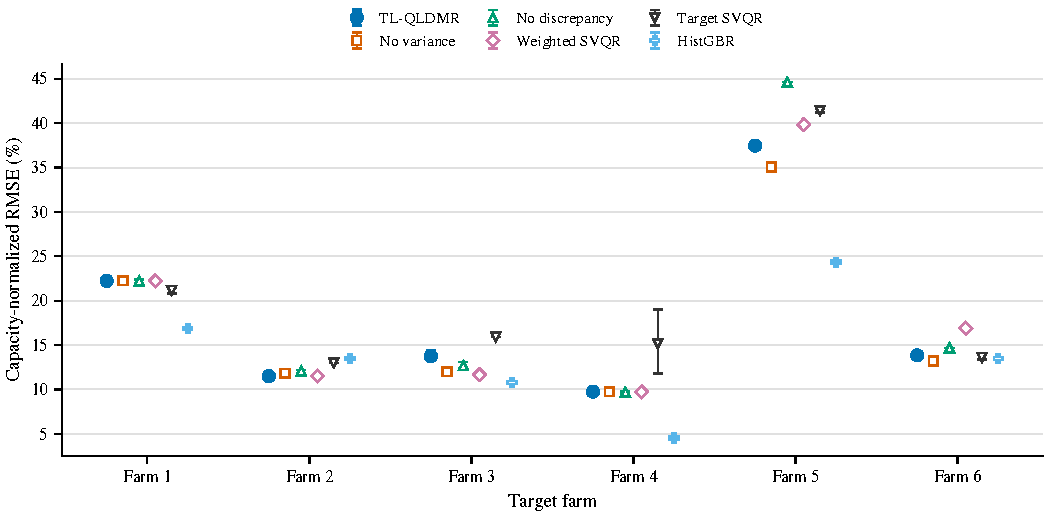
\includegraphics[width=\linewidth]{figures/within_site_normalized_rmse.pdf}
\caption{\textcolor{blue}{Capacity-normalized Q3--Q4 RMSE on the six primary within-site normal-to-extreme tasks. All methods and prespecified seeds are retained. For a kernel method, the marker is the mean of its three separate-seed RMSE values and the error bar spans their minimum and maximum; HistGBR is deterministic. These seed ranges describe algorithmic sensitivity and are not confidence intervals.}}
\label{fig:selection-v2-within-rmse}
\end{figure}

\begin{figure}[pos=htbp]
\centering
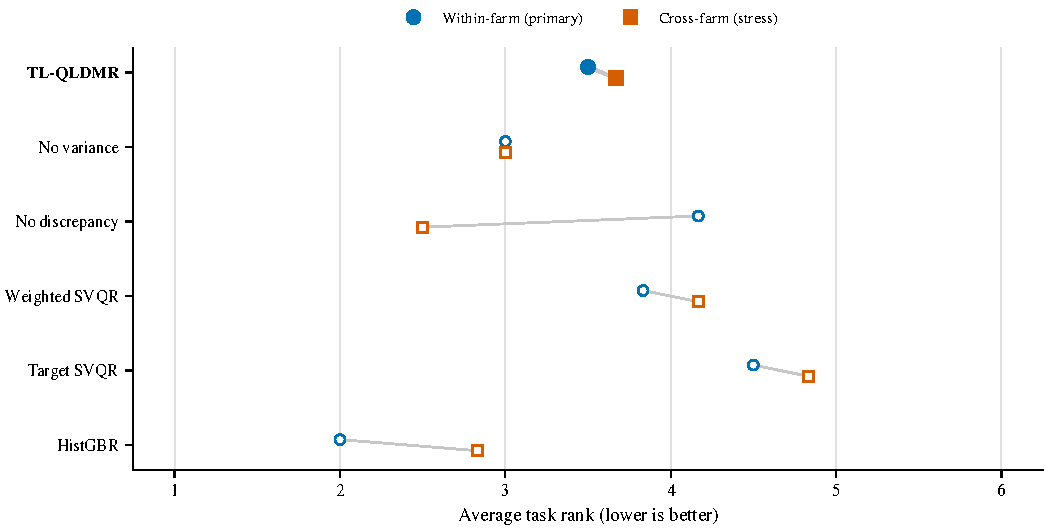
\includegraphics[width=\linewidth]{figures/scope_average_rank.pdf}
\caption{\textcolor{blue}{Average task rank in the primary within-site and secondary cross-site scopes. Ranks are computed from each task's seed-mean RMSE before equal averaging over the six sites in a scope; lower values are better.}}
\label{fig:selection-v2-scope-rank}
\end{figure}

{\color{blue}In the primary within-site scope, HistGBR was the empirical winner on the macro RMSE endpoint at 13.913\%. TL-QLDMR recorded a site-equal capacity-normalized RMSE of 18.090\%, an average task rank of 3.50, and 1 task win including ties, ranking 3rd of six by the observed macro endpoint. In the secondary cross-site stress scope, HistGBR was the empirical winner on the macro RMSE endpoint at 14.923\%. TL-QLDMR recorded a site-equal capacity-normalized RMSE of 17.694\%, an average task rank of 3.67, and 1 task win including ties, ranking 5th of six by the observed macro endpoint.}
% END SELECTION BLOCK selection_results

% BEGIN SELECTION BLOCK selection_point_inference
\subsubsection{Paired temporal-block inference}
{\color{blue}For every task and timestamp, we first average squared error over each method's declared evaluation seeds and then subtract the comparator's value from the TL-QLDMR value; negative differences favor TL-QLDMR. The timestamps are partitioned into non-overlapping Monday--Sunday seven-calendar-day blocks. We use 10,000 whole-block bootstrap resamples for a percentile 95\% interval and 99,999 two-sided paired block sign flips with a plus-one correction. Holm adjustment is applied in two separate families of 30 tests, one for the six primary tasks and one for the six secondary tasks, with five TL-QLDMR comparisons per task. The bootstrap treats block effects as approximately independent and exchangeable, while the sign-flip test additionally requires approximate sign symmetry under the null.}

{\color{blue}As a complementary scope-level summary, all 15 method pairs are compared using 99,999 two-sided seven-day block swaps of the exact site-equal capacity-normalized seed-mean macro-RMSE endpoint, with Holm adjustment applied separately within each scope. When a pair contains deterministic HistGBR, its single timewise error curve is compared with each kernel seed curve under the same block swaps; this preserves the declared seed-mean endpoint and does not treat the repeated deterministic curve as independent replication. The conservative first tier contains the empirical endpoint winner and every method whose inferiority to that winner is not established by the predeclared strict adjusted-$p<0.05$ exclusion rule. Membership indicates non-rejection of inferiority under this block procedure; it is not evidence of equivalence, does not establish superiority, and is not a formal model-confidence set.}

{\color{blue}The conservative first tier in the primary within-site scope contained HistGBR, No variance, and No discrepancy; TL-QLDMR was excluded ($p_{\mathrm{Holm}}=0.036$), meaning that its inferiority to HistGBR was established for the macro RMSE endpoint. Membership means that inferiority to the empirical winner was not established; it does not establish equivalence or equal performance. The conservative first tier in the secondary cross-site stress scope contained HistGBR, No discrepancy, No variance, Weighted SVQR, and TL-QLDMR; TL-QLDMR was retained ($p_{\mathrm{Holm}}=0.336$), meaning that its inferiority to HistGBR was not established. Membership means that inferiority to the empirical winner was not established; it does not establish equivalence or equal performance. The Holm-significant scope-level TL-QLDMR relations were: In the primary within-site scope, TL-QLDMR's observed macro RMSE was 4.178 percentage points higher than HistGBR; the all-pairs difference was significant after Holm adjustment ($p_{\mathrm{Holm}}=0.036$). In the secondary cross-site stress scope, TL-QLDMR's observed macro RMSE was 0.511 percentage points higher than No variance; the all-pairs difference was significant after Holm adjustment ($p_{\mathrm{Holm}}=0.016$). These tests concern the prespecified macro endpoint; empirical ordering by itself is not a significance claim.}

{\color{blue}The Holm-significant TL-QLDMR comparisons were: Farm~1 (within-site): TL-QLDMR had lower squared error than No variance (MSE difference, TL-QLDMR minus No variance, $-0.292$ MW$^2$; 95\% block-bootstrap CI $[-0.539, -0.139]$, $p_{\mathrm{Holm}}=0.016$). Farm~1 (within-site): TL-QLDMR had higher squared error than HistGBR (MSE difference, TL-QLDMR minus HistGBR, $204.912$ MW$^2$; 95\% block-bootstrap CI $[71.894, 425.012]$, $p_{\mathrm{Holm}}=0.012$). Farm~3 (within-site): TL-QLDMR had higher squared error than HistGBR (MSE difference, TL-QLDMR minus HistGBR, $71.623$ MW$^2$; 95\% block-bootstrap CI $[35.870, 114.080]$, $p_{\mathrm{Holm}}=0.011$). Farm~1 (cross-site): TL-QLDMR had higher squared error than HistGBR (MSE difference, TL-QLDMR minus HistGBR, $214.556$ MW$^2$; 95\% block-bootstrap CI $[91.628, 413.791]$, $p_{\mathrm{Holm}}=0.001$). Farm~6 (cross-site): TL-QLDMR had higher squared error than No variance (MSE difference, TL-QLDMR minus No variance, $16.917$ MW$^2$; 95\% block-bootstrap CI $[9.148, 27.398]$, $p_{\mathrm{Holm}}<0.001$). All other predeclared TL-QLDMR comparisons were not significant after adjustment; this absence of rejection is not evidence of equal performance.}

{\color{blue}Table~\ref{tab:selection-v2-full-inference} retains all task-level TL-QLDMR comparisons, including nonsignificant and adverse effects. The test period is reused and the number of temporal blocks is limited, so these paired results are interpreted conservatively.}

% END SELECTION BLOCK selection_point_inference

% BEGIN SELECTION BLOCK ablation
\subsubsection{Matched component removal}
{\color{blue}We use a frozen matched ablation on all twelve tasks to separate component removal from retuning. The four matched configurations, their shared fit-only artifact hashes, and the matched-analysis specification are locked before any main or matched Q3--Q4 evaluation. This point-only analysis uses $\tau=0.5$ and no Q2 labels. Within each task and seed, the TL-QLDMR-selected kernel bandwidth, total loss mass, target fraction, requested rank, fitting rows, preprocessing, landmarks, and feature map are held fixed. The no-variance, no-discrepancy, and weighted-SVQR variants differ only by setting $\lambda_1$, $\lambda_2$, or both coefficients to zero. No additional Q1 query is made. This design estimates removal effects conditional on the configuration selected for TL-QLDMR and is distinct from the independently tuned procedure comparison above.}

{\color{blue}The matched analysis retains all four variants, all twelve tasks, and seeds 0, 1, and 2. It reports site-equal capacity-normalized macro RMSE and mean rank among the four matched variants, separately for the two scopes. At the task level, we subtract each removal variant's seed-averaged squared error from that of TL-QLDMR; negative differences favor TL-QLDMR. The resulting differences use the same seven-calendar-day blocks, 10,000 whole-block bootstrap resamples, and 99,999 two-sided sign flips, with Holm adjustment in separate families of 18 tests for the primary and secondary scopes. Failure to reject a removal effect is not evidence of equivalence, and a conditional removal effect does not establish the ordering of the independently retuned procedures.}

\begin{table}[pos=t]
\centering
\color{blue}
\caption{Matched component ablation on all twelve tasks. Values are three-seed mean RMSE (MW); every removal uses the corresponding task's locked TL-QLDMR configuration and artifacts.}
\label{tab:selection-v2-matched-ablation}
\small
\setlength{\tabcolsep}{4pt}
\begin{tabular}{llrrrr}
\toprule
Scope & Farm & TL-QLDMR & No variance & No discrepancy & Weighted SVQR \\
\midrule
Within & Farm 1 & 22.012 & 22.019 & 22.014 & 22.019 \\
 & Farm 2 & 23.003 & 23.003 & 23.003 & 23.003 \\
 & Farm 3 & 13.607 & 13.759 & 13.608 & 13.759 \\
 & Farm 4 & 6.430 & 6.430 & 6.423 & 6.423 \\
 & Farm 5 & 13.488 & 13.401 & 17.534 & 17.600 \\
 & Farm 6 & 13.300 & 12.110 & 13.300 & 12.110 \\
\midrule
Cross & Farm 1 & 22.555 & 22.555 & 22.555 & 22.555 \\
 & Farm 2 & 24.127 & 24.127 & 24.127 & 24.127 \\
 & Farm 3 & 12.642 & 12.500 & 12.677 & 12.596 \\
 & Farm 4 & 5.068 & 5.068 & 5.068 & 5.068 \\
 & Farm 5 & 13.594 & 13.596 & 13.594 & 13.596 \\
 & Farm 6 & 12.586 & 12.583 & 12.670 & 12.670 \\
\bottomrule
\end{tabular}
\end{table}


{\color{blue}Under the conditional matched-removal protocol in the within-site scope, the four aggregate results were No variance 17.870\% (mean rank 2.17); TL-QLDMR 18.090\% (mean rank 2.00); Weighted SVQR 19.813\% (mean rank 3.17); No discrepancy 19.963\% (mean rank 2.67). TL-QLDMR ranked 2nd of four by observed macro RMSE. Under the conditional matched-removal protocol in the cross-site stress scope, the four aggregate results were No variance 17.671\% (mean rank 2.50); TL-QLDMR 17.694\% (mean rank 2.17); Weighted SVQR 17.702\% (mean rank 3.00); No discrepancy 17.715\% (mean rank 2.33). TL-QLDMR ranked 2nd of four by observed macro RMSE. The Holm-significant conditional removal effects were: Farm~1 (within-site): TL-QLDMR had lower squared error than No variance (MSE difference, TL-QLDMR minus No variance, $-0.292$ MW$^2$; 95\% block-bootstrap CI $[-0.524, -0.142]$, $p_{\mathrm{Holm}}=0.008$). Farm~6 (within-site): TL-QLDMR had lower squared error than No discrepancy (MSE difference, TL-QLDMR minus No discrepancy, $-4.432\times 10^{-5}$ MW$^2$; 95\% block-bootstrap CI $[-5.832\times 10^{-5}, -3.030\times 10^{-5}]$, $p_{\mathrm{Holm}}<0.001$). The observed magnitude is practically negligible on the MW$^2$ scale. These contrasts hold the TL-QLDMR-selected configuration, fitting rows, preprocessing, landmarks, and feature map fixed; variants were not independently retuned, and a failure to reject does not establish equivalence.}
% END SELECTION BLOCK ablation

% BEGIN SELECTION BLOCK selection_optimization_results
\subsubsection{Optimization accounting}
{\color{blue}The frozen design contains 72 task--method selections and 54 newly queried effective configurations per selection, for 3,888 Q1 configuration queries. The five kernel procedures require three selection-seed fits per query and HistGBR one deterministic fit, giving 10,368 required validation fits before any certificate retry. A carried incumbent may compete at a later stage using its cached Q1 score but is neither refitted nor counted as a new query. Appendix Table~\ref{tab:selection-v2-optimization-summary} accounts for every newly queried candidate and reports, by scope and method, the query and eligibility counts, failed seed certificates, solver attempts, iterations, and recorded fitting time. Because task workers can run concurrently and feature maps are cached across variants, summed fit time is descriptive and is not used to rank deployment speed.}

{\color{blue}The audited Q1 search issued 3,888 distinct within-task--method configuration queries (54 per pair) and 10,368 fit records; 3,455 queried candidates were eligible under the frozen selection rule. Among 9,720 kernel seed fits, 1,214 still missed the fixed-feature primal--dual-gap certificate after the predeclared retry and therefore made their candidate ineligible; 8,506 kernel seed fits met the certificate. Across kernel and HistGBR fits, the records contain 12,691 solver attempts and 32,207,875 reported iterations. Summed per-fit recorded time was 50.70 h. This sum is descriptive because tasks ran in parallel; it is neither elapsed wall-clock time nor inference latency. The certificate applies only to the chosen fixed-feature objective and does not certify Nyström approximation error or predictive generalization.}
% END SELECTION BLOCK selection_optimization_results

% BEGIN SELECTION BLOCK probabilistic_multiquantile
\subsubsection{Legacy exploratory multi-quantile analysis}
{\color{blue}The within-Farm~6 nine-quantile experiment is retained as a separate exploratory probability sensitivity analysis. It predates the frozen formal protocol and uses the earlier 13-variable, 24-lag input track, giving 312 meteorological inputs. In this track, pooled methods use 7,500 source fitting windows, and every method uses all 2,076 target fitting labels. The archived legacy artifacts label TL-QLDMR as ``Full''. The predefined quantile grid is}
\begin{equation*}
{\color{blue}\mathcal{T}=\{0.025,0.05,0.10,0.25,0.50,0.75,0.90,0.95,0.975\}.}
\end{equation*}

{\color{blue}Each kernel procedure receives one reference configuration $(\gamma,A,p,\lambda_1,\lambda_2)=(0.003,1000,0.5,1,1)$ and 15 fixed Latin-hypercube configurations. Their ranges are $\gamma\in[10^{-4},10^{-1}]$, total loss mass $A\in[10^2,10^5]$, target fraction $p\in[0.05,0.95]$, and active regularizer coefficients in $[10^{-2},10^3]$; all coordinates except $p$ use logarithmic scales. The Latin-hypercube design uses fixed seed 20261022, and every legacy kernel candidate uses 128 requested landmarks. Source and target loss coefficients are $C_S=A(1-p)/n_S$ and $C_T=Ap/n_T$, inactive regularizer coordinates are ignored, and target-only SVQR uses $p=1$ and $C_T=A/n_T$. With the same fixed seed, HistGBR receives 16 configurations sampled without replacement from the Cartesian grid formed by learning rates $\{0.03,0.1\}$, leaf limits $\{7,15,31\}$, minimum leaf counts $\{10,20,40\}$, $L_2$ weights $\{0,1,10\}$, iteration counts $\{100,200\}$, and target fractions $\{0.1,0.5,0.9\}$. This legacy track uses fitting-only equal-row preprocessing, so domain influence follows the available row counts, and ordinary unweighted K-means on the sampled landmark pool; it does not use the explicit one-half source/one-half target weights of the formal comparison.}

{\color{blue}Candidates are scored by unweighted mean Q1 pinball loss over all nine quantiles. Ties use the fixed candidate index, and the archived legacy rule does not filter candidates by convergence status. The 96 method--candidate records comprise 864 seed-0 quantile fits, and all six settings are locked before any Q2 calibration or Q3--Q4 prediction. The selected kernel settings are then evaluated at landmark seeds 0, 1, and 2, while deterministic HistGBR uses seed 0. Equal candidate counts specify this legacy probability-selection budget but do not imply equal model capacity or computational cost. The six selected settings are reported with the legacy audit material in Appendix Table~\ref{tab:probabilistic_configs}.}

{\color{blue}Raw quantile forecasts are retained for quantile-specific pinball loss, empirical reliability, and crossing diagnostics. A fixed label-free monotone rearrangement sorts the nine forecasts within each row before nested intervals and the weighted interval score are calculated. Q2 scores provide a fixed split-conformal expansion separately for the 50\%, 80\%, 90\%, and 95\% central intervals. The past-only rolling rule starts from Q2, uses at most the 256 most recent scores available before each forecast, and appends the current Q3--Q4 score only after that forecast has been issued. No Q3--Q4 label selects a configuration or the monotone-rearrangement rule; the fixed expansion uses Q2 alone, whereas each rolling expansion may use outcomes revealed strictly before that forecast.}

{\color{blue}The archived selection lock records the six selected configurations, and the saved validation, calibration, and test artifacts are covered by a post-completion integrity inventory. The original run manifest did not freeze the temporal loader, the target-sampling helper, the source-workbook hashes, the chronological-reference manifest, or the complete software environment; it recorded only selected source hashes and the Python and NumPy versions. This legacy analysis also uses the previously examined Q3--Q4 period. We therefore classify it as legacy/post hoc exploratory evidence rather than part of the formal point comparison or matched component analysis; its pinball loss, WIS, reliability, crossing, coverage, width, and paired-WIS results do not provide independent confirmation.}

{\color{blue}Table~\ref{tab:probabilistic_scores} shows that HistGBR has the lowest raw nine-quantile mean pinball loss (1.767\,MW) and rearranged WIS (3.531\,MW), followed by target-only SVQR (1.995 and 3.971\,MW). TL-QLDMR (Full) gives 2.045 and 4.090\,MW. Its raw crossing rate is zero, as is that of the no-discrepancy variant, whereas the other four methods cross on 38.07\%--45.84\% of test rows. This ordering stability does not translate into the lowest proper score or calibration error: TL-QLDMR's rearranged reliability MACE is 8.66 percentage points, compared with 7.35 for the no-variance and weighted-SVQR fits. These results do not establish a general probabilistic advantage for the complete objective.}

{\color{blue}For TL-QLDMR (Full), fixed Q2 calibration gives PICP values 0.532, 0.894, 0.960, and 0.977 at nominal coverages 0.50, 0.80, 0.90, and 0.95, with widths 11.21, 30.86, 41.52, and 54.75\,MW (Table~\ref{tab:probabilistic_coverage}). Figure~\ref{fig:probabilistic_reliability} reports all nine reliability points before and after rearrangement, while Fig.~\ref{fig:probabilistic_coverage} shows the static coverage--width trade-off without selecting methods or levels by test performance. Past-only rolling results are retained in the table as a separate information setting.}

{\color{blue}Paired probability-score inference uses the same 25 seven-day calendar blocks. WIS is computed separately for every seed and forecast, then averaged across landmark seeds within that forecast before forming paired method differences. The WIS difference (TL-QLDMR minus comparator) is $-0.0009$\,MW against the no-discrepancy variant (95\% block-bootstrap interval $[-0.0014,-0.0004]$, Holm $p=0.0058$), a statistically detectable but practically negligible difference. Against HistGBR the difference is $0.5585$\,MW ($[0.3290,0.8272]$, Holm $p=0.0020$), favoring HistGBR. The other three adjusted comparisons are not significant. Table~\ref{tab:probabilistic_inference} retains all five effects and tests. The block bootstrap treats block effects as approximately independent and exchangeable; the sign-flip test additionally requires approximate sign symmetry under the null. The small number of blocks and reused test period therefore require conservative interpretation.}


\begin{table}[pos=htbp]
\centering
\color{blue}
\small
\caption{\textcolor{blue}{Legacy exploratory Farm~6 evaluation on nine quantiles. Kernel entries are means over three landmark seeds; HistGBR uses its deterministic seed-0 fit. Selection uses Q1 mean pinball loss (MPL); test MPL is computed on unrearranged forecasts. WIS and calibration error use the fixed row-wise monotone rearrangement. Crossing is retained from raw forecasts. Lower scores and calibration error are preferable.}}
\label{tab:probabilistic_scores}
\resizebox{\linewidth}{!}{%
\begin{tabular}{lrrrrrr}
\toprule
Method & Candidate & Q1 MPL & Test MPL & WIS (MW) & MACE (pp) & Crossing (\%) \\
\midrule
Full & c12 & 2.432 & 2.045 & 4.090 & 8.66 & 0.00 \\
No variance & c11 & 2.435 & 2.093 & 4.168 & 7.35 & 45.81 \\
No discrepancy & c12 & 2.433 & 2.045 & 4.090 & 8.66 & 0.00 \\
Weighted SVQR & c11 & 2.435 & 2.093 & 4.169 & 7.35 & 45.84 \\
Target SVQR & c13 & 2.754 & 1.995 & 3.971 & 8.09 & 38.07 \\
HistGBR & c03 & 2.369 & 1.767 & 3.531 & 8.73 & 41.60 \\
\bottomrule
\end{tabular}}
\end{table}

\begin{table}[pos=htbp]
\centering
\color{blue}
\small
\caption{\textcolor{blue}{Legacy exploratory Farm~6 interval calibration. Each cell gives PICP/MPIW, where MPIW is in MW. S uses fixed Q2 calibration and R is the past-only 256-score rolling update.}}
\label{tab:probabilistic_coverage}
\resizebox{\linewidth}{!}{%
\begin{tabular}{llrrrr}
\toprule
Method & Calibration & 50\% & 80\% & 90\% & 95\% \\
\midrule
Full & S & 0.532/11.21 & 0.894/30.86 & 0.960/41.52 & 0.977/54.75 \\
Full & R & 0.514/11.20 & 0.855/26.19 & 0.956/39.65 & 0.984/61.92 \\
\addlinespace
No variance & S & 0.505/11.69 & 0.807/24.20 & 0.916/34.84 & 0.959/43.75 \\
No variance & R & 0.528/12.83 & 0.847/26.72 & 0.939/36.68 & 0.970/51.07 \\
\addlinespace
No discrepancy & S & 0.532/11.20 & 0.894/30.87 & 0.960/41.52 & 0.977/54.75 \\
No discrepancy & R & 0.514/11.20 & 0.855/26.19 & 0.956/39.65 & 0.984/61.92 \\
\addlinespace
Weighted SVQR & S & 0.505/11.69 & 0.807/24.20 & 0.916/34.85 & 0.959/43.75 \\
Weighted SVQR & R & 0.529/12.83 & 0.847/26.72 & 0.939/36.68 & 0.970/51.08 \\
\addlinespace
Target SVQR & S & 0.444/8.63 & 0.853/22.37 & 0.933/32.70 & 0.981/46.56 \\
Target SVQR & R & 0.481/10.79 & 0.816/22.00 & 0.922/32.42 & 0.959/49.71 \\
\addlinespace
HistGBR & S & 0.498/9.73 & 0.854/20.98 & 0.930/32.55 & 0.974/60.11 \\
HistGBR & R & 0.528/10.32 & 0.858/21.09 & 0.935/32.72 & 0.973/60.66 \\
\bottomrule
\end{tabular}}
\end{table}


\begin{figure}[pos=htbp]
\centering
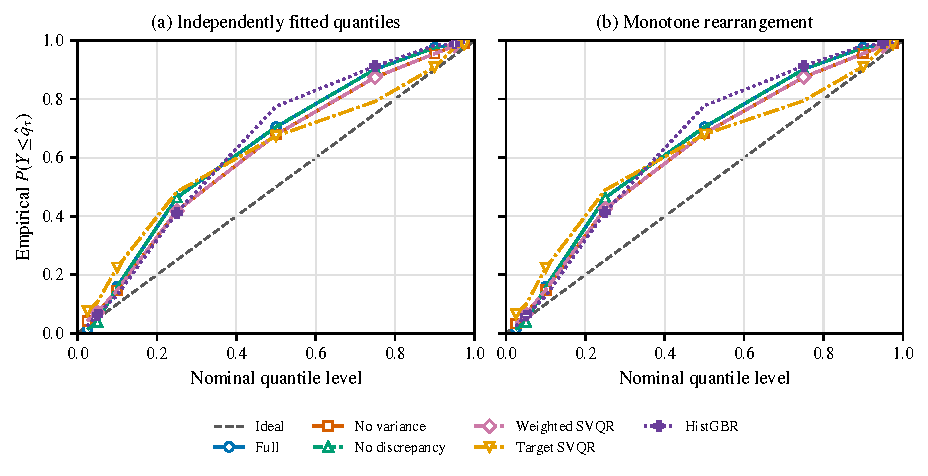
\includegraphics[width=\linewidth]{figures/probabilistic_reliability.pdf}
\caption{\textcolor{blue}{Legacy Farm~6 reliability for the probability-selected configurations. All six methods and nine predefined levels are retained; panel (a) uses the independently fitted quantiles and panel (b) applies the fixed row-wise monotone rearrangement.}}
\label{fig:probabilistic_reliability}
\end{figure}

\begin{figure}[pos=htbp]
\centering
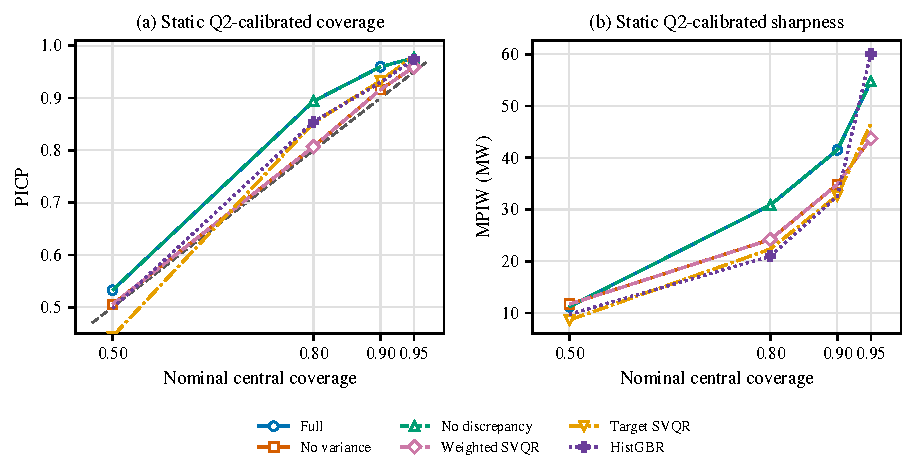
\includegraphics[width=\linewidth]{figures/probabilistic_coverage_sharpness.pdf}
\caption{\textcolor{blue}{Legacy Farm~6 fixed-Q2 interval calibration: empirical coverage and mean interval width at the four predefined nominal levels. Width is interpreted together with coverage.}}
\label{fig:probabilistic_coverage}
\end{figure}

\begin{table}[pos=htbp]
\centering
\color{blue}
\small
\caption{\textcolor{blue}{Legacy exploratory paired seven-day-block inference for probability-selected Farm~6 forecasts. Effects are Full minus comparator WIS in MW; negative values favor Full. $p_{\rm H}$ is Holm-adjusted across five comparisons.}}
\label{tab:probabilistic_inference}
\resizebox{\linewidth}{!}{%
\begin{tabular}{lrrr}
\toprule
Comparator & WIS difference & 95\% block-bootstrap interval & $p_{\rm H}$ \\
\midrule
No variance & -0.0786 & [-0.4509, 0.2679] & 1.0000 \\
No discrepancy & -0.0009 & [-0.0014, -0.0004] & 0.0058 \\
Weighted SVQR & -0.0790 & [-0.4610, 0.2644] & 1.0000 \\
Target SVQR & 0.1188 & [-0.3864, 0.5919] & 1.0000 \\
HistGBR & 0.5585 & [0.3290, 0.8272] & 0.0020 \\
\bottomrule
\end{tabular}}
\end{table}

% END SELECTION BLOCK probabilistic_multiquantile

% BEGIN SELECTION BLOCK sequential_calibration
\subsubsection{Earlier reused-test interval calibration}
{\color{blue}In the earlier point-selected two-quantile diagnostic, two calibration protocols distinguish batch forecasting from sequential operation. The fixed protocol uses all Q2 target scores and the common expansion rule defined above. Past-only rolling calibration starts with the most recent 256 available Q2 scores (or all scores when fewer are available). Before target forecast $t$, the expansion is the $\lceil(n_t+1)0.95\rceil$-th ordered score in this buffer. Only after producing the interval is its observed outcome used to append a new score and discard the oldest score if needed. The point and quantile models remain fixed. All six methods use this same rule. The past-only rolling evaluation assumes earlier target outcomes are available before the next evaluated forecast and therefore consumes additional labels during testing; it is a different information setting from fixed calibration. Neither temporal protocol inherits an exchangeability-based coverage guarantee.}
% END SELECTION BLOCK sequential_calibration

% BEGIN SELECTION BLOCK selection_calibration_results
\subsubsection{Earlier exploratory cross-farm calibration}
{\color{blue}In this earlier point-selected diagnostic, fixed Q2 calibration for TL-QLDMR (Full in the archived artifacts) produces cross-farm PICP from 0.640 to 0.988. The lowest fixed-Q2 coverage occurs on Farm~5. Past-only recalibration raises its mean PICP from 0.640 to 0.917 and reduces mean Winkler score from 44.591 to 36.547\,MW, but it does not reach 0.95. Across the other five farms, rolling PICP ranges from 0.948 to 0.962. The adjustment can widen or narrow intervals as recent scores change: for example, the TL-QLDMR mean width on Farm~5 increases from 30.760 to 33.319\,MW, while that on Farm~6 decreases from 84.673 to 83.233\,MW. Figure~\ref{fig:selected_calibration} displays both coverage and capacity-normalized width. This exploratory comparison reports performance under past-only score updating; it is not a coverage guarantee, does not identify temporal drift as a cause, and uses more outcome information than fixed Q2 calibration.}

\begin{figure}[pos=htbp]
\centering
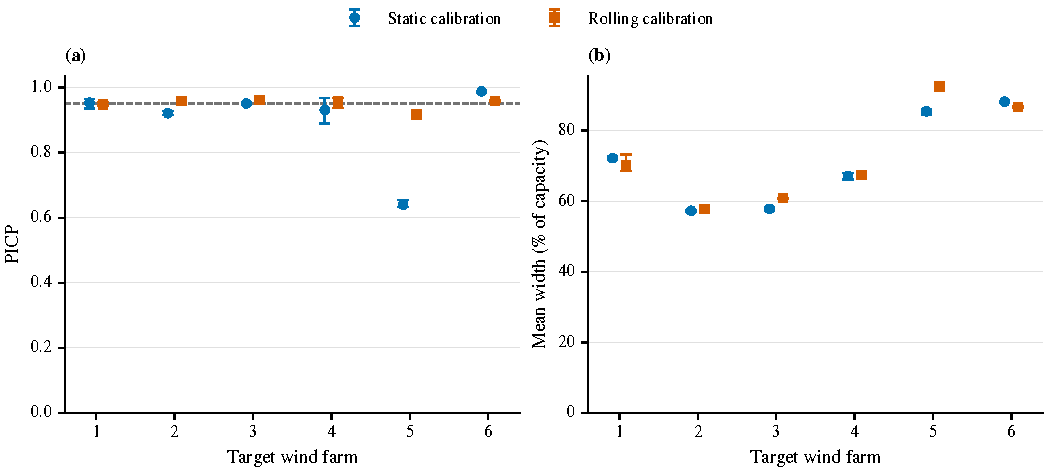
\includegraphics[width=\linewidth]{figures/selection_calibration.pdf}
\caption{\textcolor{blue}{Earlier exploratory TL-QLDMR (Full) fixed-Q2 and past-only rolling calibration across six target farms: (a) PICP and (b) mean interval width normalized by farm capacity. Points are three-seed means with minimum--maximum bars. The dashed line is nominal 0.95 coverage.}}
\label{fig:selected_calibration}
\end{figure}
\FloatBarrier
% END SELECTION BLOCK selection_calibration_results

\subsubsection{Earlier exploratory residual diagnostics}
% Numerical rows generated by review/summarize_residual_diagnostics.py; surrounding status text was revised for the formal evidence hierarchy.
% BEGIN SELECTION BLOCK selection_residual_diagnostics
{\color{blue}Table~\ref{tab:selected_residual_diagnostics} reports an earlier exploratory diagnostic from the 16-candidate, 128-landmark Farm~6 validation track, covering all 2,233 forecasts in its reused Q3--Q4 period. Residual is observed minus predicted power. Skewness and excess kurtosis are empirical standardized central moments. Tail frequency uses the fixed descriptive threshold $|e|>0.20P_{\rm nominal}=19.2$\,MW, and $Q_{0.95}(|e|)$ reports tail magnitude without binning. Each statistic is computed within each landmark seed and then averaged; HistGBR is deterministic. This analysis predates the frozen twelve-task comparison and is not used for model selection, formal predictive comparison, component attribution, or significance claims. Quantile reliability error is reported separately in Table~\ref{tab:probabilistic_scores}, because calibration is a property of the multi-quantile forecasts rather than of point residual density.}

\begin{table}[pos=htbp]
\centering
\caption{\textcolor{blue}{Earlier exploratory Farm~6 residual diagnostics. Tail frequency is the percentage with absolute error above 19.2\,MW.}}
\label{tab:selected_residual_diagnostics}
{\color{blue}\small
\resizebox{\linewidth}{!}{%
\begin{tabular}{lrrrrrrr}
\toprule
Method & Runs & Mean (MW) & SD (MW) & Skew. & Excess kurt. & $Q_{0.95}(|e|)$ (MW) & Tail (\%) \\
\midrule
Full & 3 & -4.916 & 11.175 & -2.908 & 16.459 & 21.767 & 6.34 \\
No variance & 3 & -3.817 & 11.200 & -3.075 & 17.764 & 21.523 & 6.51 \\
No discrepancy & 3 & -4.921 & 11.175 & -2.908 & 16.456 & 21.772 & 6.36 \\
Weighted SVQR & 3 & -3.817 & 11.201 & -3.074 & 17.763 & 21.532 & 6.49 \\
Target-only SVQR & 3 & -3.785 & 11.225 & -3.177 & 18.156 & 21.406 & 6.31 \\
HistGBR & 1 & -3.840 & 10.382 & -2.898 & 17.342 & 20.069 & 5.73 \\
\bottomrule
\end{tabular}}}
\end{table}
% END SELECTION BLOCK selection_residual_diagnostics


\FloatBarrier


\paragraph{\textcolor{blue}{Scope of the remaining analyses.}}
{\color{blue}The experiments that follow retain the earlier 13-variable input track and fixed reference configuration. They probe component removal, cross-farm transfer, target-label scarcity, domain weighting, meteorological-tail definitions, temporal and meteorological subsets, and computational scaling. These experiments are interpreted as descriptive sensitivity analyses and are not combined with the formal primary or secondary endpoints.}

% BEGIN STUDY BLOCK chronological_components
\subsection{\textcolor{blue}{Fixed-setting component sensitivity}}
{\color{blue}Tables~\ref{tab:chronological_components_point} and \ref{tab:chronological_components_interval} report all four variants and all three seeds on the same 2,233 target test windows. Full-model mean RMSE is 12.383799 MW, compared with 12.352255 MW without variance, 12.389858 MW without projected discrepancy, and 12.878027 MW for target-only fitting. The variance term does not improve mean RMSE at this configuration. Full-model mean coverage is 0.978952 and mean width is 49.831044 MW; target-only fitting gives coverage 0.972682, width 41.148553 MW, and a lower mean Winkler score (64.713291 versus 67.038129 MW). Thus point and interval criteria do not establish a uniform model ranking.}

\begin{table}[pos=htbp]
\centering
\color{blue}
\small
\caption{\textcolor{blue}{Component evaluation at common settings: seed mean [minimum, maximum].}}
\label{tab:chronological_components_point}
\resizebox{\linewidth}{!}{%
\begin{tabular}{lllllll}
\toprule
Variant & Runs & $n_{test}$ & RMSE (MW) & MAE (MW) & $R^2$ & Fit (s) \\
\midrule
Full & 3 & 2233 & 12.384 [12.277, 12.538] & 7.592 [7.420, 7.831] & 0.888 [0.885, 0.890] & 7.72 [6.93, 8.98] \\
NoVariance & 3 & 2233 & 12.352 [12.214, 12.527] & 7.551 [7.409, 7.782] & 0.888 [0.885, 0.891] & 7.07 [6.85, 7.31] \\
No discrepancy & 3 & 2233 & 12.390 [12.323, 12.470] & 7.594 [7.496, 7.739] & 0.888 [0.886, 0.889] & 7.40 [7.05, 8.08] \\
TargetOnly & 3 & 2233 & 12.878 [12.566, 13.077] & 7.799 [7.499, 7.957] & 0.879 [0.875, 0.884] & 5.51 [5.44, 5.56] \\
\bottomrule
\end{tabular}}
\end{table}

\begin{table}[pos=htbp]
\centering
\color{blue}
\small
\caption{\textcolor{blue}{Component evaluation at common settings: seed mean [minimum, maximum].}}
\label{tab:chronological_components_interval}
\resizebox{\linewidth}{!}{%
\begin{tabular}{lllllll}
\toprule
Variant & Runs & $n_{test}$ & PICP & MPIW (MW) & Winkler (MW) & Fit (s) \\
\midrule
Full & 3 & 2233 & 0.979 [0.975, 0.985] & 49.831 [48.596, 51.909] & 67.038 [66.187, 68.405] & 14.69 [14.20, 15.26] \\
NoVariance & 3 & 2233 & 0.976 [0.974, 0.980] & 47.907 [47.126, 49.310] & 65.973 [65.636, 66.495] & 14.99 [13.97, 15.86] \\
No discrepancy & 3 & 2233 & 0.976 [0.973, 0.981] & 48.751 [47.275, 50.409] & 66.645 [65.600, 67.754] & 14.02 [13.78, 14.32] \\
TargetOnly & 3 & 2233 & 0.973 [0.968, 0.982] & 41.149 [38.901, 45.348] & 64.713 [64.016, 65.710] & 10.83 [10.64, 10.99] \\
\bottomrule
\end{tabular}}
\end{table}

\FloatBarrier
% END STUDY BLOCK chronological_components

% BEGIN STUDY BLOCK chronological_crossfarm
\subsection{\textcolor{blue}{Fixed-setting cross-farm sensitivity}}
{\color{blue}Each site is evaluated as the target in turn. Sources are 2019 normal-domain observations from the other five sites, capped at 6,000 per source site by deterministic time-even subsampling (30,000 in total). A seed-0 subset of 128 target-site training-period meteorological-tail labels supports supervised adaptation. Power is normalized by the corresponding site's capacity before common fitting-only standardization, and predictions are converted back to the target site's MW scale. The paired target-only fit uses exactly the same target fitting labels, its own preprocessing and landmarks, and at least the full model's number of Adam updates. The effective feature dimensions are 256 for the full model and 128 for target-only fitting, which has only 128 fitting inputs. Both receive 7,552 Adam updates. These compare complete fitting procedures, including different preprocessing, feature maps, and residual-variance domains; they do not isolate a causal effect of adding source labels. All target calibration labels are additional to the 128 fitting labels and are counted in the interval table. This is supervised cross-farm adaptation, not transfer to a site with no labeled target data. Full/target-only RMSE pairs for sites 1--6 are 19.880752/23.218175, 27.819462/24.956039, 11.485825/14.297631, 5.302804/6.559925, 10.702967/17.443978, and 13.775753/13.097317 MW. The source-inclusive Full procedure has lower test RMSE on four sites and higher test RMSE on sites 2 and 6 at this fixed setting. Full-model interval coverage ranges from 0.563889 on site 5 to 1.000000 on site 4, despite the nominal calibration target of 0.95. The gains and losses demonstrate heterogeneous transfer behavior, while the coverage variation reveals substantial temporal calibration error on some sites.}

\begin{table}[pos=htbp]
\centering
\color{blue}
\small
\caption{\textcolor{blue}{Cross-farm supervised adaptation with exactly 128 target fitting labels; source normals come from the other five farms. Target-only fitting uses the same selected labels. Interval calibration labels are additional and reported separately. Fixed parameters are not claimed optimal.}}
\label{tab:chronological_crossfarm_point}
\resizebox{\linewidth}{!}{%
\begin{tabular}{lllllllll}
\toprule
Site & Variant & $n_S$ & $n_T$ & $n_{cal}$ & $n_{test}$ & RMSE (MW) & MAE (MW) & $R^2$ \\
\midrule
1 & Full & 30000 & 128 & 0 & 973 & 19.881 & 13.142 & 0.669 \\
1 & TargetOnly & 0 & 128 & 0 & 973 & 23.218 & 15.858 & 0.548 \\
2 & Full & 30000 & 128 & 0 & 901 & 27.819 & 18.156 & 0.738 \\
2 & TargetOnly & 0 & 128 & 0 & 901 & 24.956 & 17.056 & 0.789 \\
3 & Full & 30000 & 128 & 0 & 1577 & 11.486 & 8.233 & 0.842 \\
3 & TargetOnly & 0 & 128 & 0 & 1577 & 14.298 & 11.082 & 0.756 \\
4 & Full & 30000 & 128 & 0 & 526 & 5.303 & 3.829 & 0.538 \\
4 & TargetOnly & 0 & 128 & 0 & 526 & 6.560 & 4.775 & 0.293 \\
5 & Full & 30000 & 128 & 0 & 720 & 10.703 & 8.279 & 0.501 \\
5 & TargetOnly & 0 & 128 & 0 & 720 & 17.444 & 16.096 & -0.326 \\
6 & Full & 30000 & 128 & 0 & 2233 & 13.776 & 8.675 & 0.861 \\
6 & TargetOnly & 0 & 128 & 0 & 2233 & 13.097 & 8.035 & 0.875 \\
\bottomrule
\end{tabular}}
\end{table}

\begin{table}[pos=htbp]
\centering
\color{blue}
\small
\caption{\textcolor{blue}{Cross-farm supervised adaptation with exactly 128 target fitting labels; source normals come from the other five farms. Target-only fitting uses the same selected labels. Interval calibration labels are additional and reported separately. Fixed parameters are not claimed optimal.}}
\label{tab:chronological_crossfarm_interval}
\resizebox{\linewidth}{!}{%
\begin{tabular}{lllllllll}
\toprule
Site & Variant & $n_S$ & $n_T$ & $n_{cal}$ & $n_{test}$ & PICP & MPIW (MW) & Winkler (MW) \\
\midrule
1 & Full & 30000 & 128 & 305 & 973 & 0.932 & 85.372 & 99.861 \\
1 & TargetOnly & 0 & 128 & 305 & 973 & 0.906 & 83.096 & 121.990 \\
2 & Full & 30000 & 128 & 102 & 901 & 0.999 & 140.008 & 140.025 \\
2 & TargetOnly & 0 & 128 & 102 & 901 & 0.976 & 130.109 & 156.217 \\
3 & Full & 30000 & 128 & 862 & 1577 & 0.942 & 57.557 & 64.117 \\
3 & TargetOnly & 0 & 128 & 862 & 1577 & 0.992 & 80.844 & 83.264 \\
4 & Full & 30000 & 128 & 319 & 526 & 1.000 & 28.198 & 28.198 \\
4 & TargetOnly & 0 & 128 & 319 & 526 & 0.966 & 23.358 & 26.895 \\
5 & Full & 30000 & 128 & 362 & 720 & 0.564 & 29.704 & 59.361 \\
5 & TargetOnly & 0 & 128 & 362 & 720 & 0.157 & 19.048 & 272.558 \\
6 & Full & 30000 & 128 & 225 & 2233 & 0.988 & 75.095 & 77.014 \\
6 & TargetOnly & 0 & 128 & 225 & 2233 & 0.947 & 37.805 & 66.404 \\
\bottomrule
\end{tabular}}
\end{table}

\FloatBarrier
% END STUDY BLOCK chronological_crossfarm

% BEGIN STUDY BLOCK chronological_scarcity
\subsection{\textcolor{blue}{Target-label scarcity sensitivity}}
{\color{blue}The source set is fixed at 32,832 windows while target fitting budgets are 16, 32, 64, 128, 256, 512, and all 2,076 labels. Each seed defines one random target ordering, so subsets are nested within that seed. Loss coefficient masses remain 500 per domain, and preprocessing excludes unused target labels. Mean RMSE in increasing budget order is 13.714772, 13.557232, 13.335648, 12.438363, 12.661963, 12.700270, and 12.383799 MW. The 16-label range is 12.466359--15.781608 MW, compared with 12.276768--12.538363 MW using all labels. The smallest budgets show higher mean error and variability, but the curve is not strictly monotonic. This analysis concerns point prediction; interval calibration would require additional target labels.}

\begin{table}[pos=htbp]
\centering
\color{blue}
\small
\caption{\textcolor{blue}{Target-label scarcity with fixed source data and matched domain loss masses; seed mean [minimum, maximum]. Only point fitting is evaluated here.}}
\label{tab:chronological_scarcity}
\resizebox{\linewidth}{!}{%
\begin{tabular}{llllllll}
\toprule
Target-label budget & Runs & $n_S$ & $n_T$ & Effective $m$ & RMSE (MW) & MAE (MW) & Fit (s) \\
\midrule
16 & 3 & 32832 & 16 & 256 & 13.715 [12.466, 15.782] & 9.140 [7.849, 11.181] & 7.90 [7.52, 8.28] \\
32 & 3 & 32832 & 32 & 256 & 13.557 [12.621, 14.254] & 8.817 [7.203, 9.629] & 7.11 [6.82, 7.67] \\
64 & 3 & 32832 & 64 & 256 & 13.336 [12.456, 14.025] & 8.570 [7.817, 9.106] & 7.16 [6.59, 8.06] \\
128 & 3 & 32832 & 128 & 256 & 12.438 [12.033, 13.243] & 7.791 [7.287, 8.707] & 6.66 [6.58, 6.82] \\
256 & 3 & 32832 & 256 & 256 & 12.662 [12.376, 13.116] & 7.781 [7.554, 8.128] & 7.41 [6.57, 7.91] \\
512 & 3 & 32832 & 512 & 256 & 12.700 [12.291, 12.998] & 7.857 [7.512, 8.044] & 6.82 [6.65, 6.96] \\
all & 3 & 32832 & 2076 & 256 & 12.384 [12.277, 12.538] & 7.592 [7.420, 7.831] & 7.72 [6.93, 8.98] \\
\bottomrule
\end{tabular}}
\end{table}
\begin{figure}[pos=htbp]
\centering
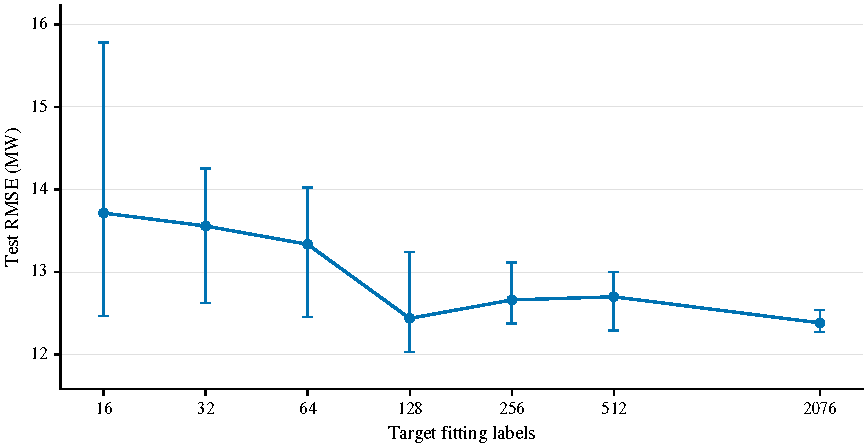
\includegraphics[width=0.85\linewidth]{figures/scarcity.pdf}
\caption{\textcolor{blue}{Target-label sensitivity on the chronological test set. Points show three-seed means and bars show the seed range.}}
\label{fig:chronological_scarcity}
\end{figure}
\FloatBarrier
% END STUDY BLOCK chronological_scarcity

% BEGIN STUDY BLOCK chronological_weighting
\subsection{\textcolor{blue}{Loss-weight allocation sensitivity}}
{\color{blue}The weighting comparison fixes $n_SC_S+n_TC_T=1000$ and seed 0, varying the allocation between domains while retaining the same fitting and test samples. Equal per-sample coefficients, equal domain masses, target/source mass ratio 10, and the historical per-sample ratios 3,000 (point) or 8,000 (interval) are compared. Domain normalization, $C_S=500/n_S$ and $C_T=500/n_T$, is identical to inverse-count imbalance compensation at this total scale, so it is not duplicated as a distinct baseline. The tables give the actual coefficients and target mass fractions. Point RMSE is 12.102063, 12.336268, 12.660232, and 12.662003 MW, respectively. The corresponding calibrated mean widths are 56.701425, 48.988181, 42.757565, and 39.768748 MW, with coverage 0.986117, 0.976265, 0.974474, and 0.965069. Target emphasis therefore changes the accuracy--coverage--width balance and does not establish an optimal weighting rule. The historical-ratio condition preserves the earlier per-sample ratios at the common total scale.}

\begin{table}[pos=htbp]
\centering
\color{blue}
\small
\caption{\textcolor{blue}{Weighting sensitivity at matched total loss weight; seed 0. Domain normalization and imbalance compensation are the same configuration at this scale.}}
\label{tab:chronological_weighting_point}
\resizebox{\linewidth}{!}{%
\begin{tabular}{lllllll}
\toprule
Scheme & $C_S$ & $C_T$ & Target mass fraction & RMSE (MW) & MAE (MW) & $R^2$ \\
\midrule
domain\_balanced & 0.01523 & 0.24085 & 0.5000 & 12.336 & 7.524 & 0.889 \\
sample\_equal & 0.02865 & 0.02865 & 0.0595 & 12.102 & 7.464 & 0.893 \\
historical\_ratio & 0.00016 & 0.47917 & 0.9948 & 12.662 & 7.654 & 0.883 \\
target\_10x & 0.00277 & 0.43791 & 0.9091 & 12.660 & 7.741 & 0.883 \\
\bottomrule
\end{tabular}}
\end{table}

\begin{table}[pos=htbp]
\centering
\color{blue}
\small
\caption{\textcolor{blue}{Weighting sensitivity at matched total loss weight; seed 0. Domain normalization and imbalance compensation are the same configuration at this scale.}}
\label{tab:chronological_weighting_interval}
\resizebox{\linewidth}{!}{%
\begin{tabular}{lllllll}
\toprule
Scheme & $C_S$ & $C_T$ & Target mass fraction & PICP & MPIW (MW) & Winkler (MW) \\
\midrule
domain\_balanced & 0.01523 & 0.24085 & 0.5000 & 0.976 & 48.988 & 66.187 \\
sample\_equal & 0.02865 & 0.02865 & 0.0595 & 0.986 & 56.701 & 67.326 \\
historical\_ratio & 0.00006 & 0.48075 & 0.9980 & 0.965 & 39.769 & 67.411 \\
target\_10x & 0.00277 & 0.43791 & 0.9091 & 0.974 & 42.758 & 67.226 \\
\bottomrule
\end{tabular}}
\end{table}

\FloatBarrier
% END STUDY BLOCK chronological_weighting

% BEGIN STUDY BLOCK chronological_thresholds
\subsection{Meteorological-tail definition sensitivity}
{\color{blue}Sensitivity uses wind upper percentiles 95, 98, and 99, paired with temperature percentiles 5/95, 2/98, and 1/99. The resulting wind thresholds are 14.17, 15.43, and 16.2588 m/s; temperature ranges are 11.16--29.97, 10.24--31.36, and 9.74--32.12 $^\circ$C. Target fitting counts are 5,004, 2,076, and 1,049; calibration counts are 683, 225, and 118; test counts are 4,600, 2,233, and 1,159. Because changing the rule changes the test population, both own-population metrics and metrics on the shared 1,159-window 99th-percentile core are reported. Core RMSE is 12.263317, 12.179039, and 12.882176 MW. Core coverage is 0.985332, 0.971527, and 0.965487, with mean widths 49.192962, 46.958026, and 43.770407 MW. All three definitions are evaluated without selecting a threshold from test performance. For each percentile definition, changing the nominal high-wind cutoff among 20, 25, and 30 m/s gives exactly the same domain mask: all percentile wind cutoffs are below 20 m/s. The union rule therefore makes these nominal high-wind cutoffs redundant; no physical turbine-shutdown comparison is available.}

\begin{table}[pos=htbp]
\centering
\color{blue}
\small
\caption{\textcolor{blue}{Threshold sensitivity on each definition's test population and the shared 99th-percentile core; seed 0. Meteorological percentiles are estimated from training observations.}}
\label{tab:chronological_thresholds_point}
\resizebox{\linewidth}{!}{%
\begin{tabular}{llllllllll}
\toprule
Percentile & Nominal cutoff (m/s) & $n_{own}$ & $n_{core}$ & Own RMSE (MW) & Own MAE (MW) & Own $R^2$ & Core RMSE (MW) & Core MAE (MW) & Core $R^2$ \\
\midrule
95 & 25 & 4600 & 1159 & 13.632 & 8.475 & 0.858 & 12.263 & 7.573 & 0.889 \\
98 & 25 & 2233 & 1159 & 12.336 & 7.524 & 0.889 & 12.179 & 7.235 & 0.890 \\
99 & 25 & 1159 & 1159 & 12.882 & 7.957 & 0.877 & 12.882 & 7.957 & 0.877 \\
\bottomrule
\end{tabular}}
\end{table}

\begin{table}[pos=htbp]
\centering
\color{blue}
\small
\caption{\textcolor{blue}{Threshold sensitivity on each definition's test population and the shared 99th-percentile core; seed 0. Meteorological percentiles are estimated from training observations.}}
\label{tab:chronological_thresholds_interval}
\resizebox{\linewidth}{!}{%
\begin{tabular}{llllllllll}
\toprule
Percentile & Nominal cutoff (m/s) & $n_{own}$ & $n_{core}$ & Own PICP & Own MPIW (MW) & Own Winkler (MW) & Core PICP & Core MPIW (MW) & Core Winkler (MW) \\
\midrule
95 & 25 & 4600 & 1159 & 0.973 & 52.921 & 72.651 & 0.985 & 49.193 & 65.414 \\
98 & 25 & 2233 & 1159 & 0.976 & 48.988 & 66.187 & 0.972 & 46.958 & 64.179 \\
99 & 25 & 1159 & 1159 & 0.965 & 43.770 & 66.428 & 0.965 & 43.770 & 66.428 \\
\bottomrule
\end{tabular}}
\end{table}

\FloatBarrier
% END STUDY BLOCK chronological_thresholds

% BEGIN STUDY BLOCK chronological_subgroups
\subsection{\textcolor{blue}{Quarter and meteorological-subset sensitivity}}
{\color{blue}The same component predictions are evaluated by test quarter and meteorological category without refitting. Q3 and Q4 contain 1,035 and 1,198 target windows; full-model mean RMSE is 5.545065 and 16.099590 MW, respectively. The high-wind, cold, and hot groups contain 955, 288, and 1,035 windows, with full-model mean RMSE 14.658582, 20.778654, and 5.545065 MW. Their mean interval coverages are 0.981501, 0.908565, and 0.995491. In this test period the hot group and Q3 target group coincide. Weather groups overlap and counts must not be added; the nominal $>25$\,m/s group is empty and has no performance estimate. Cold-subset undercoverage and the large quarterly error difference limit a general robustness claim. These observations cover two calendar quarters and overlapping sample-level categories, rather than a complete seasonal or independent-storm evaluation.}

\begin{table}[pos=htbp]
\centering
\color{blue}
\small
\caption{\textcolor{blue}{Component results by test quarter: seed mean [minimum, maximum].}}
\label{tab:chronological_quarter_point}
\resizebox{\linewidth}{!}{%
\begin{tabular}{lllllll}
\toprule
Group & Variant & Runs & $n$ & RMSE (MW) & MAE (MW) & $R^2$ \\
\midrule
2020Q3 & Full & 3 & 1035 & 5.545 [5.238, 6.042] & 4.002 [3.828, 4.341] & 0.578 [0.501, 0.625] \\
2020Q3 & NoVariance & 3 & 1035 & 5.471 [5.222, 5.796] & 3.961 [3.832, 4.181] & 0.590 [0.541, 0.628] \\
2020Q3 & No discrepancy & 3 & 1035 & 5.561 [5.185, 5.995] & 4.000 [3.756, 4.296] & 0.576 [0.509, 0.633] \\
2020Q3 & TargetOnly & 3 & 1035 & 5.543 [5.495, 5.627] & 3.940 [3.882, 4.010] & 0.580 [0.568, 0.588] \\
2020Q4 & Full & 3 & 1198 & 16.100 [16.005, 16.171] & 10.693 [10.523, 10.846] & -0.334 [-0.346, -0.318] \\
2020Q4 & NoVariance & 3 & 1198 & 16.078 [15.953, 16.231] & 10.654 [10.500, 10.893] & -0.330 [-0.356, -0.310] \\
2020Q4 & No discrepancy & 3 & 1198 & 16.104 [16.087, 16.119] & 10.698 [10.654, 10.728] & -0.334 [-0.337, -0.332] \\
2020Q4 & TargetOnly & 3 & 1198 & 16.810 [16.374, 17.108] & 11.132 [10.584, 11.478] & -0.455 [-0.506, -0.380] \\
\bottomrule
\end{tabular}}
\end{table}

\begin{table}[pos=htbp]
\centering
\color{blue}
\small
\caption{\textcolor{blue}{Component results by test quarter: seed mean [minimum, maximum].}}
\label{tab:chronological_quarter_interval}
\resizebox{\linewidth}{!}{%
\begin{tabular}{lllllll}
\toprule
Group & Variant & Runs & $n$ & PICP & MPIW (MW) & Winkler (MW) \\
\midrule
2020Q3 & Full & 3 & 1035 & 0.995 [0.988, 1.000] & 40.368 [39.695, 40.982] & 40.465 [39.971, 40.996] \\
2020Q3 & NoVariance & 3 & 1035 & 0.996 [0.993, 0.999] & 39.345 [38.750, 39.727] & 39.384 [38.834, 39.760] \\
2020Q3 & No discrepancy & 3 & 1035 & 0.993 [0.992, 0.993] & 39.902 [39.125, 40.902] & 40.032 [39.324, 40.995] \\
2020Q3 & TargetOnly & 3 & 1035 & 0.992 [0.989, 0.997] & 28.288 [27.133, 30.121] & 28.767 [27.865, 30.199] \\
2020Q4 & Full & 3 & 1198 & 0.965 [0.956, 0.972] & 58.006 [55.174, 61.829] & 89.996 [88.576, 92.576] \\
2020Q4 & NoVariance & 3 & 1198 & 0.959 [0.952, 0.968] & 55.304 [53.664, 58.434] & 88.945 [87.992, 90.393] \\
2020Q4 & No discrepancy & 3 & 1198 & 0.962 [0.956, 0.971] & 56.396 [53.838, 60.158] & 89.637 [87.909, 92.316] \\
2020Q4 & TargetOnly & 3 & 1198 & 0.956 [0.948, 0.968] & 52.260 [48.656, 58.504] & 95.768 [95.248, 96.390] \\
\bottomrule
\end{tabular}}
\end{table}

\begin{table}[pos=htbp]
\centering
\color{blue}
\small
\caption{\textcolor{blue}{Component results by meteorological subset: seed mean [minimum, maximum]. Subsets may overlap; dashes indicate an empty subset.}}
\label{tab:chronological_weather_point}
\resizebox{\linewidth}{!}{%
\begin{tabular}{lllllll}
\toprule
Group & Variant & Runs & $n$ & RMSE (MW) & MAE (MW) & $R^2$ \\
\midrule
high\_wind & Full & 3 & 955 & 14.659 [14.527, 14.774] & 10.418 [10.228, 10.599] & -0.473 [-0.496, -0.446] \\
high\_wind & NoVariance & 3 & 955 & 14.633 [14.486, 14.841] & 10.375 [10.202, 10.650] & -0.468 [-0.509, -0.438] \\
high\_wind & No discrepancy & 3 & 955 & 14.673 [14.650, 14.690] & 10.430 [10.373, 10.460] & -0.475 [-0.479, -0.471] \\
high\_wind & TargetOnly & 3 & 955 & 15.157 [14.687, 15.487] & 10.731 [10.182, 11.097] & -0.575 [-0.644, -0.478] \\
cold & Full & 3 & 288 & 20.779 [20.741, 20.830] & 12.288 [12.194, 12.340] & -0.203 [-0.209, -0.199] \\
cold & NoVariance & 3 & 288 & 20.760 [20.676, 20.816] & 12.255 [12.151, 12.369] & -0.201 [-0.207, -0.191] \\
cold & No discrepancy & 3 & 288 & 20.752 [20.666, 20.823] & 12.262 [12.211, 12.287] & -0.200 [-0.208, -0.190] \\
cold & TargetOnly & 3 & 288 & 22.289 [21.864, 22.555] & 13.579 [12.987, 13.884] & -0.384 [-0.417, -0.332] \\
hot & Full & 3 & 1035 & 5.545 [5.238, 6.042] & 4.002 [3.828, 4.341] & 0.578 [0.501, 0.625] \\
hot & NoVariance & 3 & 1035 & 5.471 [5.222, 5.796] & 3.961 [3.832, 4.181] & 0.590 [0.541, 0.628] \\
hot & No discrepancy & 3 & 1035 & 5.561 [5.185, 5.995] & 4.000 [3.756, 4.296] & 0.576 [0.509, 0.633] \\
hot & TargetOnly & 3 & 1035 & 5.543 [5.495, 5.627] & 3.940 [3.882, 4.010] & 0.580 [0.568, 0.588] \\
$>25$\,m/s & Full & 3 & 0 & --- & --- & --- \\
$>25$\,m/s & NoVariance & 3 & 0 & --- & --- & --- \\
$>25$\,m/s & No discrepancy & 3 & 0 & --- & --- & --- \\
$>25$\,m/s & TargetOnly & 3 & 0 & --- & --- & --- \\
\bottomrule
\end{tabular}}
\end{table}

\begin{table}[pos=htbp]
\centering
\color{blue}
\small
\caption{\textcolor{blue}{Component results by meteorological subset: seed mean [minimum, maximum]. Subsets may overlap; dashes indicate an empty subset.}}
\label{tab:chronological_weather_interval}
\resizebox{\linewidth}{!}{%
\begin{tabular}{lllllll}
\toprule
Group & Variant & Runs & $n$ & PICP & MPIW (MW) & Winkler (MW) \\
\midrule
high\_wind & Full & 3 & 955 & 0.982 [0.981, 0.982] & 60.895 [58.014, 64.826] & 77.531 [74.829, 81.167] \\
high\_wind & NoVariance & 3 & 955 & 0.980 [0.979, 0.981] & 58.234 [56.585, 61.462] & 75.633 [73.655, 78.516] \\
high\_wind & No discrepancy & 3 & 955 & 0.981 [0.980, 0.981] & 59.227 [56.530, 63.151] & 76.619 [74.496, 80.408] \\
high\_wind & TargetOnly & 3 & 955 & 0.973 [0.970, 0.978] & 55.565 [51.884, 61.886] & 79.093 [77.864, 81.400] \\
cold & Full & 3 & 288 & 0.909 [0.872, 0.941] & 46.294 [43.681, 49.785] & 130.682 [128.842, 133.446] \\
cold & NoVariance & 3 & 288 & 0.890 [0.865, 0.924] & 43.470 [41.893, 46.314] & 132.450 [129.202, 136.636] \\
cold & No discrepancy & 3 & 288 & 0.896 [0.872, 0.934] & 44.835 [42.693, 48.068] & 132.322 [131.248, 133.590] \\
cold & TargetOnly & 3 & 288 & 0.878 [0.851, 0.924] & 38.679 [35.326, 44.684] & 154.833 [146.947, 160.070] \\
hot & Full & 3 & 1035 & 0.995 [0.988, 1.000] & 40.368 [39.695, 40.982] & 40.465 [39.971, 40.996] \\
hot & NoVariance & 3 & 1035 & 0.996 [0.993, 0.999] & 39.345 [38.750, 39.727] & 39.384 [38.834, 39.760] \\
hot & No discrepancy & 3 & 1035 & 0.993 [0.992, 0.993] & 39.902 [39.125, 40.902] & 40.032 [39.324, 40.995] \\
hot & TargetOnly & 3 & 1035 & 0.992 [0.989, 0.997] & 28.288 [27.133, 30.121] & 28.767 [27.865, 30.199] \\
$>25$\,m/s & Full & 3 & 0 & --- & --- & --- \\
$>25$\,m/s & NoVariance & 3 & 0 & --- & --- & --- \\
$>25$\,m/s & No discrepancy & 3 & 0 & --- & --- & --- \\
$>25$\,m/s & TargetOnly & 3 & 0 & --- & --- & --- \\
\bottomrule
\end{tabular}}
\end{table}

\FloatBarrier
% END STUDY BLOCK chronological_subgroups

% BEGIN STUDY BLOCK chronological_scalability
\subsection{\textcolor{blue}{Landmark and source-size sensitivity}}
{\color{blue}The landmark curve uses $m=32,64,128,256,512,1024$ with unchanged fitting/test samples and all three seeds. Mean RMSE is 12.859364, 12.495129, 12.552243, 12.383799, 12.343112, and 12.284720 MW; corresponding mean fitting times are 1.22, 1.95, 3.55, 7.72, 15.61, and 33.45 s. The source-size experiment retains 2,076 target fitting labels and uses 3,283, 8,208, 16,416, or 32,832 time-even source samples at seed 0. Coefficients are renormalized to the same domain masses at each scale. The figure shows all specified sample sizes and landmark counts, with seed ranges for repeated fits. Increasing the landmark count increases measured cost and changes predictive accuracy, but the accuracy curve is not strictly monotonic. These are fixed-epoch empirical trade-offs. Because feature dimension, dataset size, and finite-step optimization can all affect the result, these curves describe empirical predictive trade-offs rather than exact-kernel approximation error. They do not measure prediction latency, peak or resident memory, online model-update cost, or GPU performance. The past-only rolling calibration experiment updates only a score buffer after outcomes arrive; it does not refit the predictor. We therefore make no real-time or deployment-throughput claim.}

\begin{table}[pos=htbp]
\centering
\color{blue}
\small
\caption{\textcolor{blue}{Accuracy--runtime trade-off with fixed training and test data; seed mean [minimum, maximum]. Time covers solver fitting only.}}
\label{tab:chronological_landmarks}
\resizebox{\linewidth}{!}{%
\begin{tabular}{llllllll}
\toprule
Requested landmarks & Runs & $n_S$ & $n_T$ & Effective $m$ & RMSE (MW) & MAE (MW) & Fit (s) \\
\midrule
32 & 3 & 32832 & 2076 & 32 & 12.859 [12.819, 12.882] & 8.231 [8.128, 8.287] & 1.22 [1.17, 1.31] \\
64 & 3 & 32832 & 2076 & 64 & 12.495 [12.240, 12.736] & 7.736 [7.490, 8.044] & 1.95 [1.84, 2.16] \\
128 & 3 & 32832 & 2076 & 128 & 12.552 [12.444, 12.683] & 7.782 [7.618, 8.020] & 3.55 [3.32, 3.82] \\
256 & 3 & 32832 & 2076 & 256 & 12.384 [12.277, 12.538] & 7.592 [7.420, 7.831] & 7.72 [6.93, 8.98] \\
512 & 3 & 32832 & 2076 & 512 & 12.343 [12.140, 12.546] & 7.529 [7.303, 7.837] & 15.61 [15.46, 15.80] \\
1024 & 3 & 32832 & 2076 & 1024 & 12.285 [12.068, 12.571] & 7.459 [7.255, 7.661] & 33.45 [31.66, 35.10] \\
\bottomrule
\end{tabular}}
\end{table}

\begin{table}[pos=htbp]
\centering
\color{blue}
\small
\caption{\textcolor{blue}{Source-size sensitivity with a fixed target training pool and test set; seed 0. Source selection is evenly spaced in training time.}}
\label{tab:chronological_source_scale}
\resizebox{\linewidth}{!}{%
\begin{tabular}{llllllll}
\toprule
Source fraction & Runs & $n_S$ & $n_T$ & Effective $m$ & RMSE (MW) & MAE (MW) & Fit (s) \\
\midrule
0.1 & 1 & 3283 & 2076 & 256 & 12.985 [12.985, 12.985] & 8.063 [8.063, 8.063] & 4.60 [4.60, 4.60] \\
0.25 & 1 & 8208 & 2076 & 256 & 12.911 [12.911, 12.911] & 8.090 [8.090, 8.090] & 4.86 [4.86, 4.86] \\
0.5 & 1 & 16416 & 2076 & 256 & 13.013 [13.013, 13.013] & 8.037 [8.037, 8.037] & 5.50 [5.50, 5.50] \\
1.0 & 1 & 32832 & 2076 & 256 & 12.336 [12.336, 12.336] & 7.524 [7.524, 7.524] & 8.98 [8.98, 8.98] \\
\bottomrule
\end{tabular}}
\end{table}
\begin{figure}[pos=htbp]
\centering
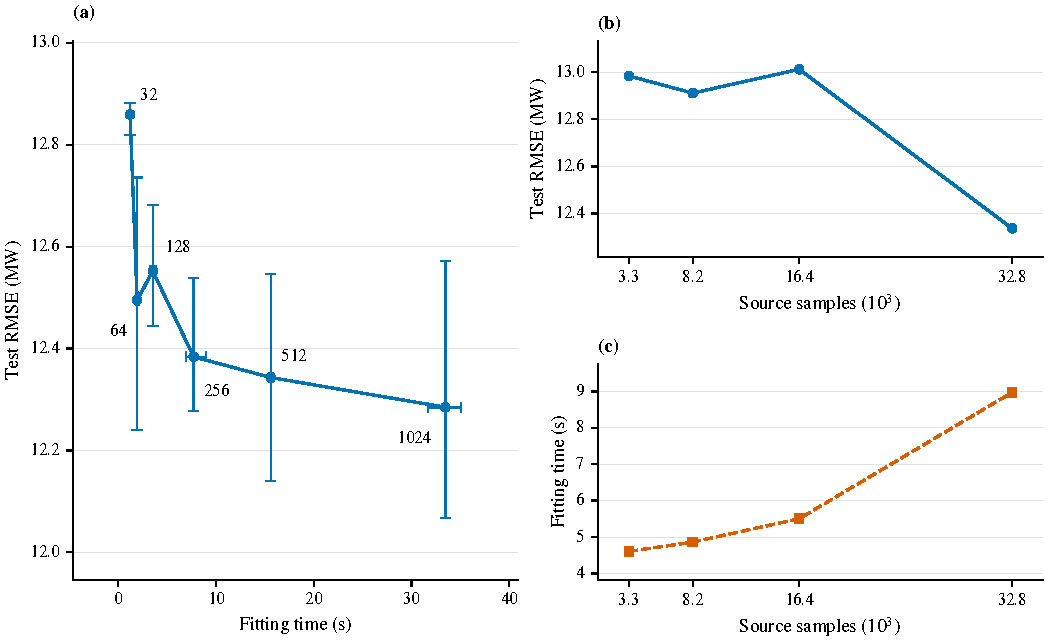
\includegraphics[width=\linewidth]{figures/chronological_accuracy_runtime.pdf}
\caption{\textcolor{blue}{Predictive accuracy and fitting cost: (a) landmark accuracy--time trade-off, (b) source-size sensitivity of RMSE, and (c) source-size sensitivity of fitting time. Landmark points show three-seed means and ranges, with labels indicating $m$; source-size results use seed 0.}}
\label{fig:chronological_accuracy_runtime}
\end{figure}
\FloatBarrier
% END STUDY BLOCK chronological_scalability


\section{Conclusion}\label{conclusion}
{\color{blue}This paper presents TL-QLDMR for wind power forecasting when labeled target-domain samples are limited and the source and target samples are defined by different meteorological selection rules. The formulation combines normalized source-residual variance, a projected inter-domain mean-discrepancy penalty, and weighted pinball loss. The variance is symmetric; quantile dependence comes from the loss. Exact-kernel and fixed Nystr\"{o}m objectives are convex under the stated kernel and parameter conditions, without a claim of joint strong convexity or a convergence rate for Adam.}


% BEGIN V2 GENERATED conclusion_evidence
{\color{blue}The implementation passes deterministic objective, gradient, and primal--dual consistency checks. In the primary within-site scope, histogram gradient boosting had the lowest observed site-equal capacity-normalized root mean squared error at 13.913\%. TL-QLDMR recorded 18.090\%, an average task rank of 3.50, and 1 task win including ties; it ranked 3rd of six and was excluded from the conservative first tier. In the secondary cross-site stress scope, histogram gradient boosting had the lowest observed site-equal capacity-normalized root mean squared error at 14.923\%. TL-QLDMR recorded 17.694\%, an average task rank of 3.67, and 1 task win including ties; it ranked 5th of six and was retained in the conservative first tier. The first-tier statements are non-rejections of inferiority to each empirical endpoint winner and do not establish equivalence, equal performance, or superiority. Among 60 predeclared task-level comparisons, 1 Holm-adjusted finding favored TL-QLDMR and 4 favored a comparator; non-rejection for the remaining comparisons does not establish equal performance. In the conditional matched-removal analysis for the primary within-site scope, TL-QLDMR recorded 18.090\% and ranked 2nd of four by macro RMSE, with the lowest mean task rank (2.00); the lowest observed matched endpoint was the no-variance variant at 17.870\%. In the conditional matched-removal analysis for the secondary cross-site stress scope, TL-QLDMR recorded 17.694\% and ranked 2nd of four by macro RMSE, with the lowest mean task rank (2.17); the lowest observed matched endpoint was the no-variance variant at 17.671\%. Across 36 matched task-level contrasts, 2 Holm-adjusted effects favored TL-QLDMR and 0 favored a removal variant. These effects are conditional on the TL-QLDMR-selected settings; the variants were not independently retuned, and non-rejection does not establish equivalence. The separate Farm~6 nine-quantile and earlier calibration studies remain legacy exploratory sensitivity analyses and are not part of the formal evidence chain. Taken together, the formal results provide a scope- and task-dependent assessment of TL-QLDMR rather than evidence of universal superiority. Because the public Q3--Q4 test period had been examined before the frozen protocol was designed, the comparison is test-locked evidence on a reused period and does not provide independent external confirmation.}
% END V2 GENERATED conclusion_evidence

{\color{blue}The formal comparison uses a public six-farm dataset whose Q3--Q4 period had been examined before the frozen protocol was designed. Locking Q1 selection, the analysis specification, and the matched configurations before evaluation prevents further test-guided adaptation, but it does not turn the reused period into independent confirmation. The 128 target labels describe the fitting budget rather than total supervision because Q1 selection and Q2 calibration labels are additional; past-only rolling calibration further uses outcomes revealed before the current forecast. Equal configuration-query counts do not equalize model capacity, solver attempts, or wall-clock cost, algorithmic seed ranges are not confidence intervals, first-tier membership establishes non-rejection rather than equivalence, and matched removal effects are conditional on the TL-QLDMR-selected configuration. Chronological ordering does not remove serial dependence or establish conformal coverage guarantees. Meteorological-tail membership is defined retrospectively from target-time weather, with overlapping sample categories rather than independently tracked storms or ramp events. The numerical certificate applies only to each fixed-feature training objective, while Nystr\"{o}m approximation error, independent-farm generalization, longer forecast horizons, and deployment latency remain unestablished. The separate Farm~6 nine-quantile analysis is legacy exploratory evidence whose original archive did not freeze every current loader, sampler, or chronological-reference dependency.}


Future work will focus on extending the framework to multi-site spatiotemporal coupling, adaptive online recalibration under non-stationary weather, and hybrid kernel-deep transfer formulations.

\FloatBarrier
\appendix
\section{Validation-selected comparison details}\label{app:selection_details}
{\color{blue}The formal frozen comparison records and the legacy probability sensitivity are grouped separately below. The formal tables retain all primary and secondary tasks, prescribed methods and seeds, paired comparisons, selected configurations, and optimization-accounting records. The legacy table reports only the earlier exploratory Farm~6 multi-quantile configuration search; it is not part of the formal point-comparison evidence.}

\subsection{Formal held-out results and paired inference}
\begin{table*}[pos=t,width=\FullWidth]
\centering
\color{blue}
\caption{Q3--Q4 RMSE (MW) for all six secondary leave-one-farm-out transfer-stress tasks. Kernel entries are means over the three predeclared evaluation seeds; HistGBR is deterministic.}
\label{tab:selection-v2-secondary-cross-rmse}
\small
\setlength{\tabcolsep}{3pt}
\begin{tabular}{lrrrrrr}
\toprule
Farm & TL-QLDMR & No variance & No discrepancy & Weighted SVQR & Target SVQR & HistGBR \\
\midrule
Farm 1 & 22.555 & 22.555 & 22.555 & 22.555 & 20.969 & 17.152 \\
Farm 2 & 24.127 & 25.145 & 24.471 & 26.108 & 25.996 & 27.898 \\
Farm 3 & 12.642 & 12.500 & 12.369 & 12.596 & 15.762 & 11.063 \\
Farm 4 & 5.068 & 4.375 & 4.364 & 4.375 & 10.008 & 4.896 \\
Farm 5 & 13.594 & 12.996 & 12.309 & 12.220 & 14.910 & 9.475 \\
Farm 6 & 12.586 & 11.895 & 12.124 & 15.593 & 13.079 & 12.813 \\
\bottomrule
\end{tabular}
\end{table*}

\FloatBarrier
{\color{blue}\small
\setlength{\tabcolsep}{3.5pt}
\begin{longtable}{lllrrr}
\caption{Paired seven-day-block inference for TL-QLDMR minus each comparator. Negative squared-error differences favor TL-QLDMR; Holm correction is applied separately within each scope.}\label{tab:selection-v2-full-inference}\\
\toprule
Scope & Farm & Comparator & $\Delta$MSE (MW$^2$) & 95\% CI & Holm $p$ \\
\midrule
\endfirsthead
\toprule
Scope & Farm & Comparator & $\Delta$MSE (MW$^2$) & 95\% CI & Holm $p$ \\
\midrule
\endhead
\midrule
\multicolumn{6}{r}{Continued on next page} \\
\endfoot
\bottomrule
\endlastfoot
Within & Farm 1 & No variance & -0.292 & [-0.539, -0.139] & 0.016 \\
Within & Farm 1 & No discrepancy & -0.088 & [-0.535, 0.305] & 1.000 \\
Within & Farm 1 & Weighted SVQR & -0.295 & [-0.804, 0.079] & 1.000 \\
Within & Farm 1 & Target SVQR & 44.794 & [-61.815, 215.850] & 1.000 \\
Within & Farm 1 & HistGBR & 204.912 & [71.894, 425.012] & 0.012 \\
Within & Farm 2 & No variance & -31.270 & [-145.378, 85.682] & 1.000 \\
Within & Farm 2 & No discrepancy & -53.861 & [-129.202, 25.260] & 1.000 \\
Within & Farm 2 & Weighted SVQR & -0.000 & [-0.000, 0.000] & 1.000 \\
Within & Farm 2 & Target SVQR & -146.629 & [-326.897, -1.156] & 1.000 \\
Within & Farm 2 & HistGBR & -196.071 & [-310.817, 95.884] & 1.000 \\
Within & Farm 3 & No variance & 44.230 & [-2.696, 101.441] & 1.000 \\
Within & Farm 3 & No discrepancy & 27.575 & [-4.420, 72.692] & 1.000 \\
Within & Farm 3 & Weighted SVQR & 51.869 & [10.609, 112.964] & 1.000 \\
Within & Farm 3 & Target SVQR & -63.095 & [-109.626, 13.183] & 1.000 \\
Within & Farm 3 & HistGBR & 71.623 & [35.870, 114.080] & 0.011 \\
Within & Farm 4 & No variance & 0.039 & [0.019, 0.055] & 0.550 \\
Within & Farm 4 & No discrepancy & 0.367 & [0.220, 0.554] & 0.214 \\
Within & Farm 4 & Weighted SVQR & 0.090 & [0.062, 0.112] & 0.195 \\
Within & Farm 4 & Target SVQR & -62.625 & [-84.807, -32.268] & 0.375 \\
Within & Farm 4 & HistGBR & 32.450 & [10.745, 78.065] & 0.291 \\
Within & Farm 5 & No variance & 22.498 & [-9.744, 55.766] & 1.000 \\
Within & Farm 5 & No discrepancy & -76.172 & [-216.164, 30.753] & 1.000 \\
Within & Farm 5 & Weighted SVQR & -23.780 & [-75.782, 46.863] & 1.000 \\
Within & Farm 5 & Target SVQR & -40.390 & [-88.126, 23.695] & 1.000 \\
Within & Farm 5 & HistGBR & 105.180 & [-18.457, 250.036] & 1.000 \\
Within & Farm 6 & No variance & 16.388 & [3.446, 30.628] & 0.586 \\
Within & Farm 6 & No discrepancy & -21.701 & [-58.089, 20.841] & 1.000 \\
Within & Farm 6 & Weighted SVQR & -86.115 & [-151.839, -17.623] & 0.794 \\
Within & Farm 6 & Target SVQR & 5.707 & [-45.029, 42.756] & 1.000 \\
Within & Farm 6 & HistGBR & 9.067 & [-19.106, 35.184] & 1.000 \\
Cross & Farm 1 & No variance & -0.000 & [-0.000, 0.000] & 1.000 \\
Cross & Farm 1 & No discrepancy & -0.000 & [-0.000, -0.000] & 1.000 \\
Cross & Farm 1 & Weighted SVQR & -0.000 & [-0.000, -0.000] & 1.000 \\
Cross & Farm 1 & Target SVQR & 68.963 & [-24.897, 223.287] & 1.000 \\
Cross & Farm 1 & HistGBR & 214.556 & [91.628, 413.791] & 0.001 \\
Cross & Farm 2 & No variance & -50.142 & [-100.394, 16.419] & 1.000 \\
Cross & Farm 2 & No discrepancy & -16.717 & [-71.262, 54.779] & 1.000 \\
Cross & Farm 2 & Weighted SVQR & -99.485 & [-172.116, -8.825] & 1.000 \\
Cross & Farm 2 & Target SVQR & -93.676 & [-204.326, 5.650] & 1.000 \\
Cross & Farm 2 & HistGBR & -196.191 & [-371.740, 140.592] & 1.000 \\
Cross & Farm 3 & No variance & 3.577 & [-8.904, 12.857] & 1.000 \\
Cross & Farm 3 & No discrepancy & 6.827 & [0.096, 13.359] & 1.000 \\
Cross & Farm 3 & Weighted SVQR & 1.166 & [-14.189, 10.437] & 1.000 \\
Cross & Farm 3 & Target SVQR & -88.613 & [-169.974, -12.707] & 1.000 \\
Cross & Farm 3 & HistGBR & 37.443 & [-5.162, 77.722] & 1.000 \\
Cross & Farm 4 & No variance & 6.552 & [4.090, 9.094] & 0.203 \\
Cross & Farm 4 & No discrepancy & 6.642 & [4.140, 9.131] & 0.208 \\
Cross & Farm 4 & Weighted SVQR & 6.553 & [4.079, 9.060] & 0.218 \\
Cross & Farm 4 & Target SVQR & -78.181 & [-98.114, -59.655] & 0.108 \\
Cross & Farm 4 & HistGBR & 1.810 & [-5.537, 6.569] & 1.000 \\
Cross & Farm 5 & No variance & 15.908 & [3.281, 32.790] & 0.518 \\
Cross & Farm 5 & No discrepancy & 33.296 & [-3.974, 77.932] & 1.000 \\
Cross & Farm 5 & Weighted SVQR & 35.477 & [7.063, 73.611] & 0.586 \\
Cross & Farm 5 & Target SVQR & -37.520 & [-101.136, 52.569] & 1.000 \\
Cross & Farm 5 & HistGBR & 95.014 & [-33.479, 254.940] & 1.000 \\
Cross & Farm 6 & No variance & 16.917 & [9.148, 27.398] & $<0.001$ \\
Cross & Farm 6 & No discrepancy & 11.377 & [1.620, 21.132] & 0.931 \\
Cross & Farm 6 & Weighted SVQR & -84.739 & [-208.359, 16.658] & 1.000 \\
Cross & Farm 6 & Target SVQR & -12.774 & [-33.757, 2.002] & 1.000 \\
Cross & Farm 6 & HistGBR & -5.764 & [-57.237, 42.540] & 1.000 \\
\end{longtable}
}


\subsection{Frozen selection and optimization audit}
\begin{table*}[pos=t,width=\FullWidth]
\centering
\color{blue}
\caption{Locked kernel configurations for the primary within-farm tasks. The source stage identifies where the retained incumbent was first queried.}
\label{tab:selection-v2-within-kernel-configs}
\small
\setlength{\tabcolsep}{3pt}
\begin{tabular}{lllrlllll}
\toprule
Farm & Method & Stage & $r$ & $\gamma$ & $A$ & $p$ & $\lambda_1$ & $\lambda_2$ \\
\midrule
Farm 1 & TL-QLDMR & middle & 512 & 0.006473 & 8.18e+05 & 0.7659 & 1000 & 1000 \\
Farm 1 & No variance & middle & 512 & 0.006473 & 8.18e+05 & 0.7659 & 0 & 1000 \\
Farm 1 & No discrepancy & middle & 512 & 0.006473 & 8.18e+05 & 0.7659 & 1000 & 0 \\
Farm 1 & Weighted SVQR & base & 512 & 0.006473 & 8.18e+05 & 0.7659 & 0 & 0 \\
Farm 1 & Target SVQR & middle & 64 & 0.004511 & 1072 & 1 & 0 & 0 \\
Farm 2 & TL-QLDMR & middle & 128 & 0.002705 & 1697 & 0.2553 & 1e-05 & 1e-05 \\
Farm 2 & No variance & joint & 512 & 0.005956 & 709.3 & 0.255 & 0 & 2.04e-05 \\
Farm 2 & No discrepancy & joint & 128 & 0.004308 & 668.2 & 0.373 & 1e-05 & 0 \\
Farm 2 & Weighted SVQR & base & 128 & 0.002705 & 1697 & 0.2553 & 0 & 0 \\
Farm 2 & Target SVQR & middle & 128 & 0.001752 & 310.3 & 1 & 0 & 0 \\
Farm 3 & TL-QLDMR & joint & 256 & 0.001972 & 1.05e+04 & 0.3023 & 1000 & 1.277 \\
Farm 3 & No variance & joint & 256 & 0.002054 & 3072 & 0.05 & 0 & 0.000799 \\
Farm 3 & No discrepancy & joint & 128 & 0.001157 & 1.15e+04 & 0.07518 & 1000 & 0 \\
Farm 3 & Weighted SVQR & joint & 512 & 0.001597 & 3268 & 0.0726 & 0 & 0 \\
Farm 3 & Target SVQR & joint & 128 & 0.001498 & 1102 & 1 & 0 & 0 \\
Farm 4 & TL-QLDMR & middle & 512 & 0.006473 & 8.18e+05 & 0.7659 & 0.02199 & 470.1 \\
Farm 4 & No variance & middle & 512 & 0.006473 & 8.18e+05 & 0.7659 & 0 & 300 \\
Farm 4 & No discrepancy & joint & 512 & 0.006495 & 2.4e+06 & 0.6455 & 5.814 & 0 \\
Farm 4 & Weighted SVQR & base & 512 & 0.006473 & 8.18e+05 & 0.7659 & 0 & 0 \\
Farm 4 & Target SVQR & joint & 64 & 0.005659 & 5.74e+05 & 1 & 0 & 0 \\
Farm 5 & TL-QLDMR & joint & 256 & 0.006236 & 3583 & 0.8431 & 1000 & 1000 \\
Farm 5 & No variance & middle & 512 & 0.003 & 1000 & 0.5 & 0 & 1000 \\
Farm 5 & No discrepancy & joint & 512 & 0.00301 & 5030 & 0.3576 & 581.4 & 0 \\
Farm 5 & Weighted SVQR & joint & 256 & 0.004746 & 100 & 0.9848 & 0 & 0 \\
Farm 5 & Target SVQR & joint & 64 & 0.004757 & 214 & 1 & 0 & 0 \\
Farm 6 & TL-QLDMR & joint & 128 & 0.000216 & 253.5 & 0.07898 & 960.1 & 9.79e-05 \\
Farm 6 & No variance & joint & 256 & 0.000854 & 232.5 & 0.06464 & 0 & 0.7989 \\
Farm 6 & No discrepancy & joint & 256 & 0.00036 & 1110 & 0.1986 & 5.488 & 0 \\
Farm 6 & Weighted SVQR & joint & 256 & 0.0001 & 1.65e+04 & 0.05602 & 0 & 0 \\
Farm 6 & Target SVQR & joint & 32 & 0.001373 & 9714 & 1 & 0 & 0 \\
\bottomrule
\end{tabular}
\end{table*}

\begin{table*}[pos=t,width=\FullWidth]
\centering
\color{blue}
\caption{Locked kernel configurations for the secondary cross-farm tasks. The source stage identifies where the retained incumbent was first queried.}
\label{tab:selection-v2-cross-kernel-configs}
\small
\setlength{\tabcolsep}{3pt}
\begin{tabular}{lllrlllll}
\toprule
Farm & Method & Stage & $r$ & $\gamma$ & $A$ & $p$ & $\lambda_1$ & $\lambda_2$ \\
\midrule
Farm 1 & TL-QLDMR & middle & 256 & 0.007981 & 1.65e+04 & 0.6965 & 1e-05 & 1e-05 \\
Farm 1 & No variance & middle & 256 & 0.007981 & 1.65e+04 & 0.6965 & 0 & 1e-05 \\
Farm 1 & No discrepancy & middle & 256 & 0.007981 & 1.65e+04 & 0.6965 & 1e-05 & 0 \\
Farm 1 & Weighted SVQR & base & 256 & 0.007981 & 1.65e+04 & 0.6965 & 0 & 0 \\
Farm 1 & Target SVQR & middle & 64 & 0.004511 & 1072 & 1 & 0 & 0 \\
Farm 2 & TL-QLDMR & joint & 512 & 0.001256 & 392.4 & 0.5023 & 1e-05 & 0.000107 \\
Farm 2 & No variance & joint & 128 & 0.002862 & 261.1 & 0.8228 & 0 & 1e-05 \\
Farm 2 & No discrepancy & joint & 256 & 0.002176 & 576.8 & 0.9039 & 350.3 & 0 \\
Farm 2 & Weighted SVQR & joint & 512 & 0.001557 & 672.7 & 0.9824 & 0 & 0 \\
Farm 2 & Target SVQR & middle & 128 & 0.001752 & 310.3 & 1 & 0 & 0 \\
Farm 3 & TL-QLDMR & middle & 512 & 0.003 & 1000 & 0.5 & 1000 & 1000 \\
Farm 3 & No variance & middle & 512 & 0.003 & 1000 & 0.5 & 0 & 1000 \\
Farm 3 & No discrepancy & joint & 512 & 0.002434 & 1983 & 0.1293 & 1000 & 0 \\
Farm 3 & Weighted SVQR & base & 512 & 0.003 & 1000 & 0.5 & 0 & 0 \\
Farm 3 & Target SVQR & joint & 128 & 0.001498 & 1102 & 1 & 0 & 0 \\
Farm 4 & TL-QLDMR & joint & 128 & 0.006992 & 9.17e+04 & 0.5067 & 1.82e-05 & 0.389 \\
Farm 4 & No variance & middle & 512 & 0.006473 & 8.18e+05 & 0.7659 & 0 & 3 \\
Farm 4 & No discrepancy & joint & 512 & 0.006495 & 2.4e+06 & 0.6455 & 5.814 & 0 \\
Farm 4 & Weighted SVQR & base & 512 & 0.006473 & 8.18e+05 & 0.7659 & 0 & 0 \\
Farm 4 & Target SVQR & joint & 64 & 0.005659 & 5.74e+05 & 1 & 0 & 0 \\
Farm 5 & TL-QLDMR & joint & 128 & 0.005784 & 1280 & 0.437 & 9.332 & 1e-05 \\
Farm 5 & No variance & joint & 128 & 0.005417 & 1039 & 0.6331 & 0 & 0.005117 \\
Farm 5 & No discrepancy & joint & 256 & 0.005414 & 366.5 & 0.8446 & 150.5 & 0 \\
Farm 5 & Weighted SVQR & joint & 256 & 0.005026 & 1358 & 0.9024 & 0 & 0 \\
Farm 5 & Target SVQR & joint & 64 & 0.004757 & 214 & 1 & 0 & 0 \\
Farm 6 & TL-QLDMR & middle & 128 & 0.003 & 1000 & 0.5 & 3.481 & 6.488 \\
Farm 6 & No variance & joint & 128 & 0.002862 & 261.1 & 0.8228 & 0 & 3.597 \\
Farm 6 & No discrepancy & joint & 128 & 0.004777 & 393.7 & 0.6344 & 0.0139 & 0 \\
Farm 6 & Weighted SVQR & middle & 256 & 0.01173 & 100 & 0.2087 & 0 & 0 \\
Farm 6 & Target SVQR & joint & 32 & 0.001373 & 9714 & 1 & 0 & 0 \\
\bottomrule
\end{tabular}
\end{table*}

\begin{table*}[pos=t,width=\FullWidth]
\centering
\color{blue}
\caption{Locked HistGBR configurations for the primary and secondary tasks.}
\label{tab:selection-v2-histgbr-configs}
\small
\setlength{\tabcolsep}{3pt}
\begin{tabular}{lllrrrrrr}
\toprule
Scope & Farm & Stage & LR & Leaves & Min. leaf & $L_2$ & Iter. & $p$ \\
\midrule
Within & Farm 1 & middle & 0.02564 & 15 & 5 & 100 & 400 & 0.9828 \\
Within & Farm 2 & joint & 0.04065 & 7 & 10 & 0 & 100 & 0.902 \\
Within & Farm 3 & base & 0.03 & 31 & 20 & 1 & 400 & 0.1 \\
Within & Farm 4 & joint & 0.2208 & 63 & 10 & 100 & 600 & 0.05 \\
Within & Farm 5 & joint & 0.04427 & 63 & 20 & 10 & 600 & 0.3008 \\
Within & Farm 6 & middle & 0.08804 & 15 & 5 & 1 & 200 & 0.7421 \\
Cross & Farm 1 & base & 0.03 & 15 & 20 & 1 & 400 & 0.995 \\
Cross & Farm 2 & base & 0.1 & 7 & 10 & 10 & 100 & 0.9 \\
Cross & Farm 3 & middle & 0.03813 & 7 & 40 & 1 & 200 & 0.1226 \\
Cross & Farm 4 & joint & 0.03994 & 63 & 5 & 100 & 600 & 0.995 \\
Cross & Farm 5 & joint & 0.09123 & 31 & 20 & 0.1 & 200 & 0.9682 \\
Cross & Farm 6 & middle & 0.1184 & 63 & 40 & 0 & 400 & 0.9526 \\
\bottomrule
\end{tabular}
\end{table*}

\begin{table*}[pos=t,width=\FullWidth]
\centering
\color{blue}
\caption{Audited Q1 optimization totals by scope and method. B, M, and J are newly queried candidates in the base, middle, and joint stages. Eligibility and certificate failures refer only to newly queried candidates. Iterations sum the reported iterations over all solver attempts; fit time sums recorded per-fit wall time and is descriptive because tasks ran in parallel.}
\label{tab:selection-v2-optimization-summary}
\small
\setlength{\tabcolsep}{3pt}
\begin{tabular}{llrrrrrrrr}
\toprule
Scope & Method & B & M & J & Eligible & Failed seed fits & Attempts & Iterations & Fit h \\
\midrule
Within & TL-QLDMR & 108 & 108 & 108 & 280 & 123 & 1287 & 4025325 & 7.07 \\
Within & No variance & 108 & 108 & 108 & 276 & 135 & 1270 & 3941850 & 6.43 \\
Within & No discrepancy & 108 & 108 & 108 & 273 & 146 & 1297 & 4217100 & 6.42 \\
Within & Weighted SVQR & 108 & 108 & 108 & 249 & 215 & 1296 & 4594600 & 5.22 \\
Within & Target SVQR & 108 & 108 & 108 & 324 & 0 & 973 & 137300 & 0.02 \\
Within & HistGBR & 108 & 108 & 108 & 324 & 0 & 324 & 97200 & 2.67 \\
Cross & TL-QLDMR & 108 & 108 & 108 & 275 & 132 & 1230 & 3563825 & 6.14 \\
Cross & No variance & 108 & 108 & 108 & 277 & 132 & 1227 & 3497425 & 4.95 \\
Cross & No discrepancy & 108 & 108 & 108 & 276 & 133 & 1220 & 3514200 & 4.69 \\
Cross & Weighted SVQR & 108 & 108 & 108 & 253 & 198 & 1270 & 4384550 & 4.69 \\
Cross & Target SVQR & 108 & 108 & 108 & 324 & 0 & 973 & 137300 & 0.02 \\
Cross & HistGBR & 108 & 108 & 108 & 324 & 0 & 324 & 97200 & 2.36 \\
\bottomrule
\end{tabular}
\end{table*}

\FloatBarrier

\subsection{Legacy exploratory probability configuration}
{\color{blue}The following configuration table belongs to the reused-test exploratory nine-quantile sensitivity analysis and is reported for auditability rather than independent confirmation.}
\begin{table}[pos=htbp]
\centering
\color{blue}
\small
\caption{\textcolor{blue}{Legacy exploratory Farm~6 configurations selected by Q1 nine-quantile mean pinball loss. For the kernel methods, $A=n_SC_S+n_TC_T$ and $p=n_TC_T/A$; inactive penalties are shown as zero, and target-only SVQR has $p=1$. HistGBR uses learning rate (LR), maximum leaves, minimum leaf size, $L_2$ weight, iterations, and target mass fraction $p$. Candidate indices are zero-based.}}
\label{tab:probabilistic_configs}
\resizebox{\linewidth}{!}{%
\begin{tabular}{lrrrrrr}
\toprule
Kernel method & ID & $\gamma$ & $A$ & $p$ & $\lambda_1$ & $\lambda_2$ \\
\midrule
Full & c12 & 0.001132 & 232.8 & 0.652 & 391.6 & 0.1011 \\
No variance & c11 & 0.0002446 & 81222.2 & 0.191 & 0 & 1.351 \\
No discrepancy & c12 & 0.001132 & 232.8 & 0.652 & 391.6 & 0 \\
Weighted SVQR & c11 & 0.0002446 & 81222.2 & 0.191 & 0 & 0 \\
Target SVQR & c13 & 0.002267 & 755.0 & 1.000 & 0 & 0 \\
\bottomrule
\end{tabular}}

\medskip
\resizebox{\linewidth}{!}{%
\begin{tabular}{lrrrrrrr}
\toprule
Tree method & ID & LR & Leaves & Min. leaf & $L_2$ & Iterations & $p$ \\
\midrule
HistGBR & c03 & 0.03 & 7 & 40 & 1.0 & 200 & 0.100 \\
\bottomrule
\end{tabular}}
\end{table}

\FloatBarrier


\FloatBarrier
% BEGIN METHOD BLOCK data_code_availability
\section*{Data and Code Availability}
{\color{blue}The raw six-farm SCADA workbooks are publicly available in version~4 of the State Grid Renewable Energy Generation dataset (data DOI: \href{https://doi.org/10.6084/m9.figshare.17304221.v4}{10.6084/m9.figshare.17304221.v4}, CC0), described in the data article cited here (DOI: \href{https://doi.org/10.1038/s41597-022-01696-6}{10.1038/s41597-022-01696-6}). Supplementary Reproducibility Package~S1 provides the code, exact identifiers, preprocessing records, finite-search records, locks, selected configurations, calibration records, row-level predictions, statistical analyses, and publication rendering for the formal 12-task comparison and its independently locked matched component ablation; both are governed by pre-evaluation locks and frozen analysis rules. S1 also retains the performance-blind numerical-certificate amendment, the original and amended records and models for its single triggering main-study fit, and the intent and completion sidecars; the objective and tolerance were unchanged, and no matched-ablation fit used the amendment. A compact inventory records package-time checksums for all bottom-level selection/main fit records after exact comparison with their embeddings; those checksums are a packaging audit rather than an original experiment lock. The earlier chronological common-setting material is identified by package-time artifact hashes, and the probability material is separately labeled legacy/posthoc with its provenance limitation; neither is represented as formal pre-evaluation evidence. The public raw workbooks and bulk regenerable fitted-model binaries are not duplicated; the small amendment audit-chain model pair is retained. The final package has 2,262 manifest entries; its external ZIP has SHA-256 \texttt{262efbf7\allowbreak{}da974020\allowbreak{}6f3a840e\allowbreak{}4adc0024\allowbreak{}0d41609c\allowbreak{}55689873\allowbreak{}afe831a2\allowbreak{}814d2b59}.}
% END METHOD BLOCK data_code_availability


%------------------------ Credit ------------------------
\printcredits


%------------------------ Declaration ------------------------
\section*{Declaration of Competing Interest}
The authors declare that they have no known competing financial interests or personal relationships that could have appeared to influence the work reported in this paper.


%------------------------ Acknowledgments ------------------------
\section*{Acknowledgments}
This work was supported in part by the National Natural Science Foundation of China under Grant 72471109 and Grant 62106205.



%------------------------ Reference ------------------------

\bibliographystyle{model5-names}
\bibliography{ref.bib}

\end{document}
